\chapter{Resultados}
\label{sec:resultados}

Este capítulo irá apresentar os resultados obtidos com a execução deste trabalho. Para tanto, optou-se mostrá-los considerando os objetivos mostrados na Seção \ref{sec:objetivos}. Deve-se observar que cada uma das seções deste capítulo corresponde a um objetivo específico definido para esta pesquisa. Para alcançar os resultados, foi necessário utilizar ferramentas de auxílio, elas encontram-se no Apêndice \ref{ap:suporte}.

\section{Seleção dos Métodos Matemáticos}

Nesta seção é evidenciado os resultados  das simulações dos \textit{experts} em linguagem MQL4 (produto da implementação dos Métodos Matemáticos), através de relatórios e gráficos gerados pela plataforma MetaTrader. Conforme estabelecido na metodologia de pesquisa, os Métodos Matemáticos que obtiveram 10\% de rendimento sob o capital inicial, foram selecionados para serem implementados no software InvestMVC. Este resultado atende o objetivo específico 1 (selecionar Métodos Matemáticos a serem implementados) deste trabalho.

\subsection{Implementação dos Métodos Matemáticos}

Os métodos de Correlação Linear, Média Móvel, Mínimos Quadrados, Estocástico e Fibonacci foram implementados em linguagem MQL4 e assim foi construído um \textit{expert} para cada método. Esses produtos de software receberam os nomes, respectivamente, CorrelacaoPearson.mql, MediaMovel.mql, MinimosQuadrados.mql, Estocastico.mql e Fibonacci.mql. Cada \textit{expert} encontra-se no Apêndice \ref{ap:experts}.

\subsection{Simulação do Método de Correlação Linear}

O \textit{expert} CorrelacaoPearson.mql obteve o percentual de negociações com lucros de 56.86\% no período de Agosto de 2012 a Agosto de 2013. Nesse período, o \textit{expert} teve um lucro de 1981.60 USD. No período de Agosto de 2013 a Agosto de 2014, o percentual de negociações com lucros foi de 55.56\%  e obteve-se o lucro de 1119.05 USD. 
Os relatórios completos das simulações podem ser visualizados nas Figuras \ref{protocoloCorrelacao} e \ref{protocoloCorrelacao2}.

\newpage
\begin{figure}[H]
\centering
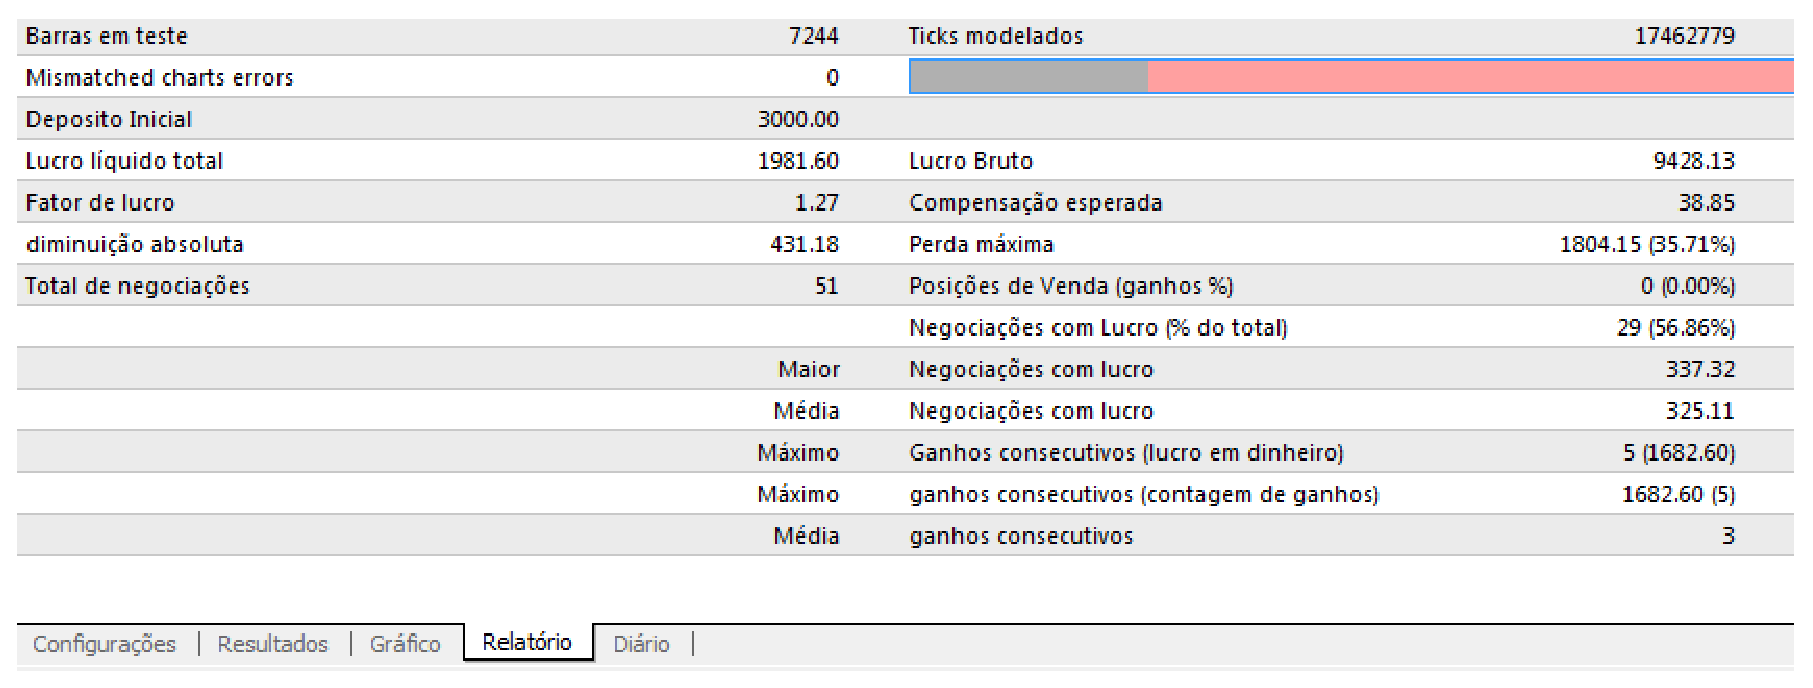
\includegraphics[width=0.9\textwidth]{figuras/protocoloCorrelacao}
\caption{Relatório de simulação no período de Agosto de 2012 a Agosto de 2013 do \textit{expert} CorrelacaoPearson.mql}
\label{protocoloCorrelacao}
\end{figure}

\begin{figure}[H]
\centering

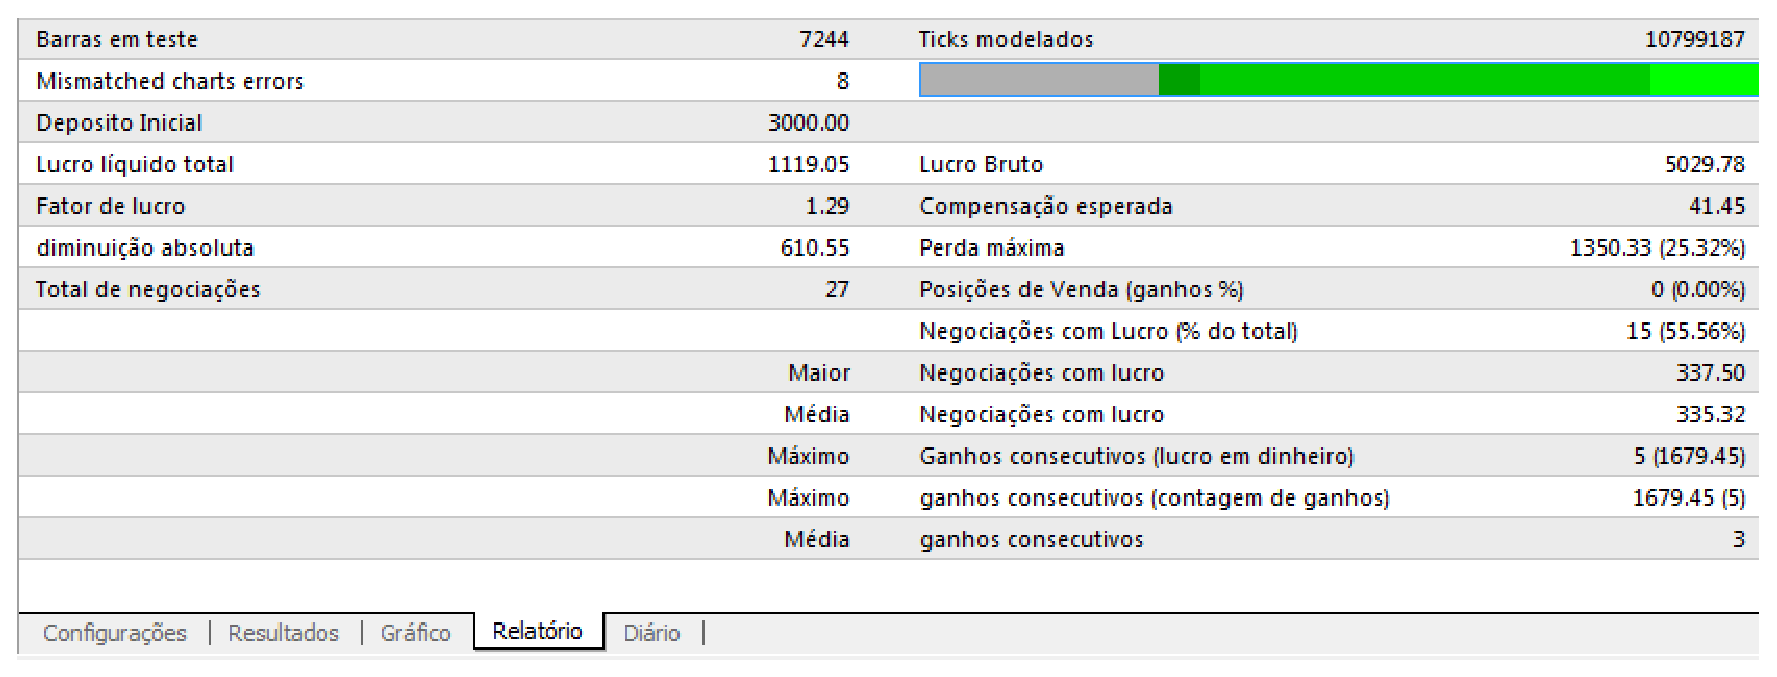
\includegraphics[width=0.9\textwidth]{figuras/protocoloCorrelacao2}
\caption{Relatório de simulação no período de Agosto de 2013 a Agosto de 2014 do \textit{expert} CorrelacaoPearson.mql}
\label{protocoloCorrelacao2}
\end{figure}

Foram gerados os gráficos de simulação de 2012 a 2013 e de 2013 a 2014, conforme ilustrado nas Figuras \ref{protocoloCorrelacao3} e \ref{protocoloCorrelacao4}. É possível perceber que o método de Correlação de Pearson perde dinheiro em alguns períodos, mas os ganhos são superiores às perdas.

\newpage
\begin{figure}[H]
\centering
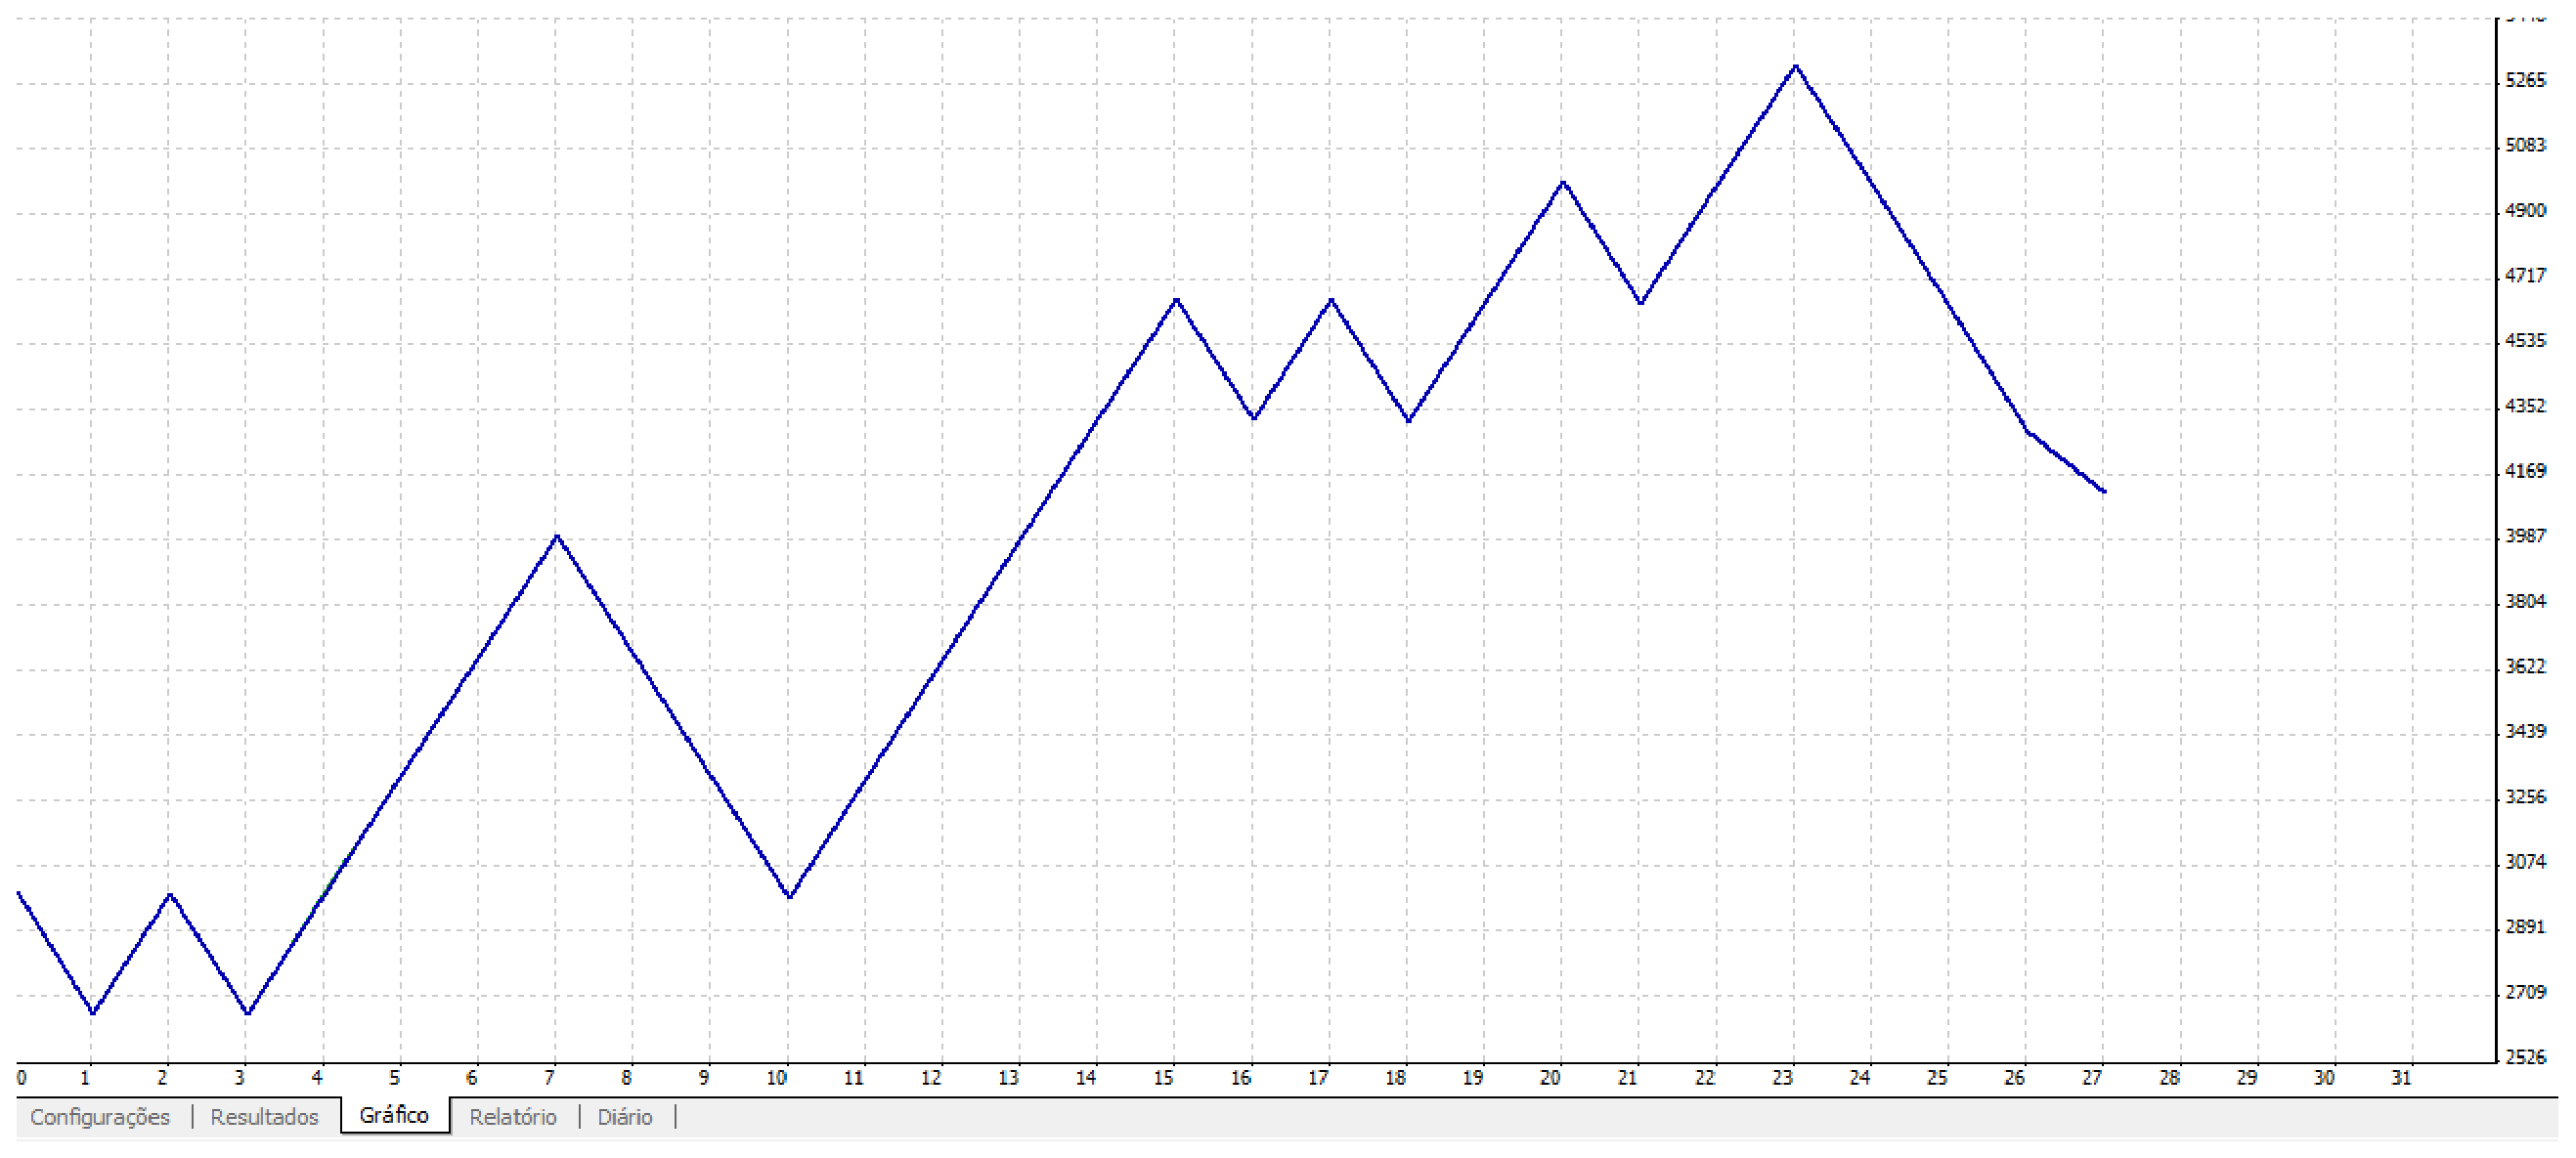
\includegraphics[width=0.9\textwidth]{figuras/protocoloCorrelacao3}
\caption{Gráfico gerado pela simulação do \textit{expert} CorrelacaoPearson.mql no período de Agosto de 2012 a Agosto de 2013}
\label{protocoloCorrelacao3}
\end{figure}

\begin{figure}[H]
\centering
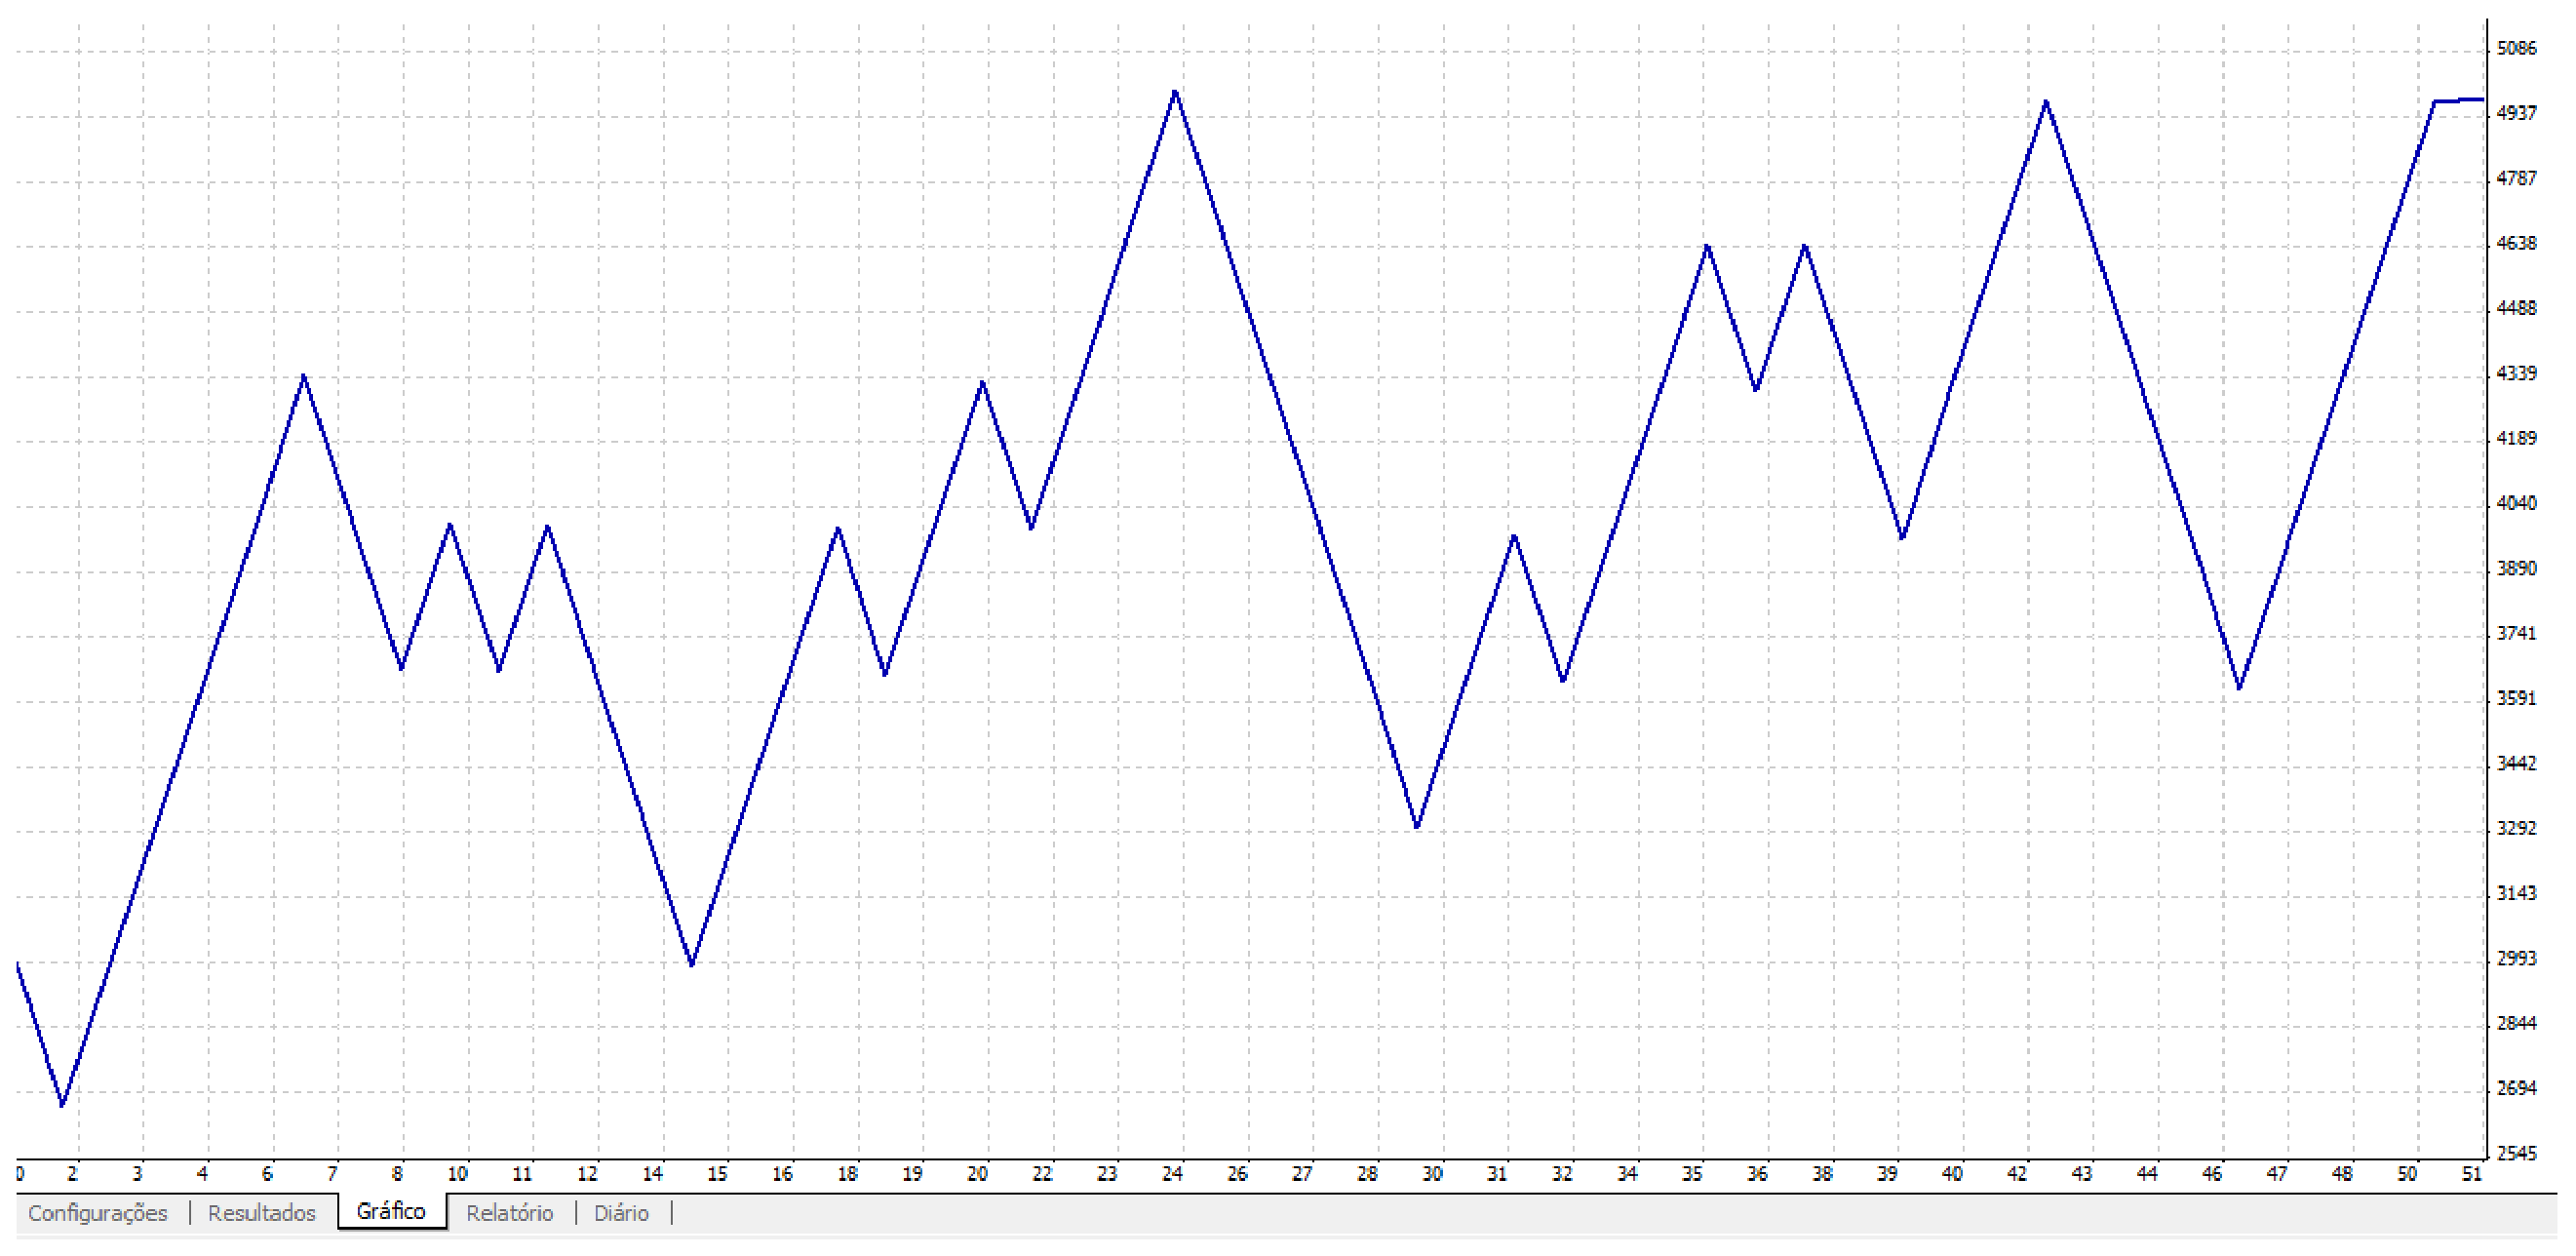
\includegraphics[width=0.9\textwidth]{figuras/protocoloCorrelacao4}
\caption{Gráfico gerado pela simulação do \textit{expert} CorrelacaoPearson.mql no período de Agosto de 2013 a Agosto de 2014}
\label{protocoloCorrelacao4}
\end{figure}

\subsection{Simulação do método de Mínimos Quadrados}

O \textit{expert} MinimosQuadrados.mql obteve o percentual de negociações com lucros de 77.88\% no período de Agosto de 2012 a Agosto de 2013, e o  lucro nesse período foi de 1341.88 USD. No período de Agosto de 2013 a Agosto de 2014, o percentual de negociações com lucros foi de 85.71\%,  e obteve-se o lucro de 1026 USD. 
Os relatórios completos das simulações podem ser visualizados nas Figuras \ref{protocoloMinimos} e \ref{protocoloMinimos2}.

\newpage
\begin{figure}[H]
\centering
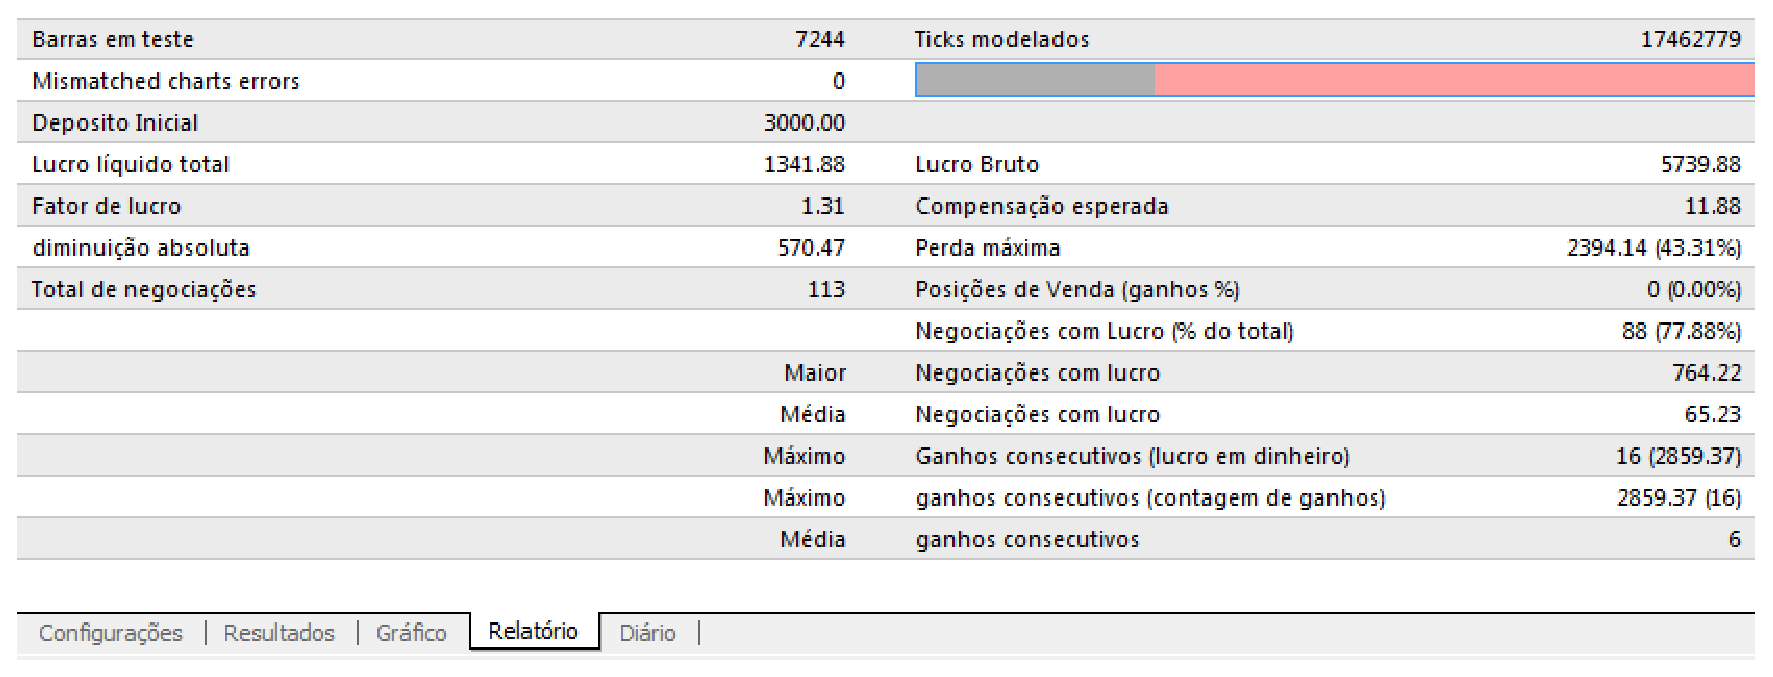
\includegraphics[width=0.9\textwidth]{figuras/protocoloMinimos}
\caption{Relatório de simulação no período de Agosto de 2012 a Agosto de 2013 do \textit{expert} MinimosQuadrados.mql}
\label{protocoloMinimos}
\end{figure}

\begin{figure}[H]
\centering
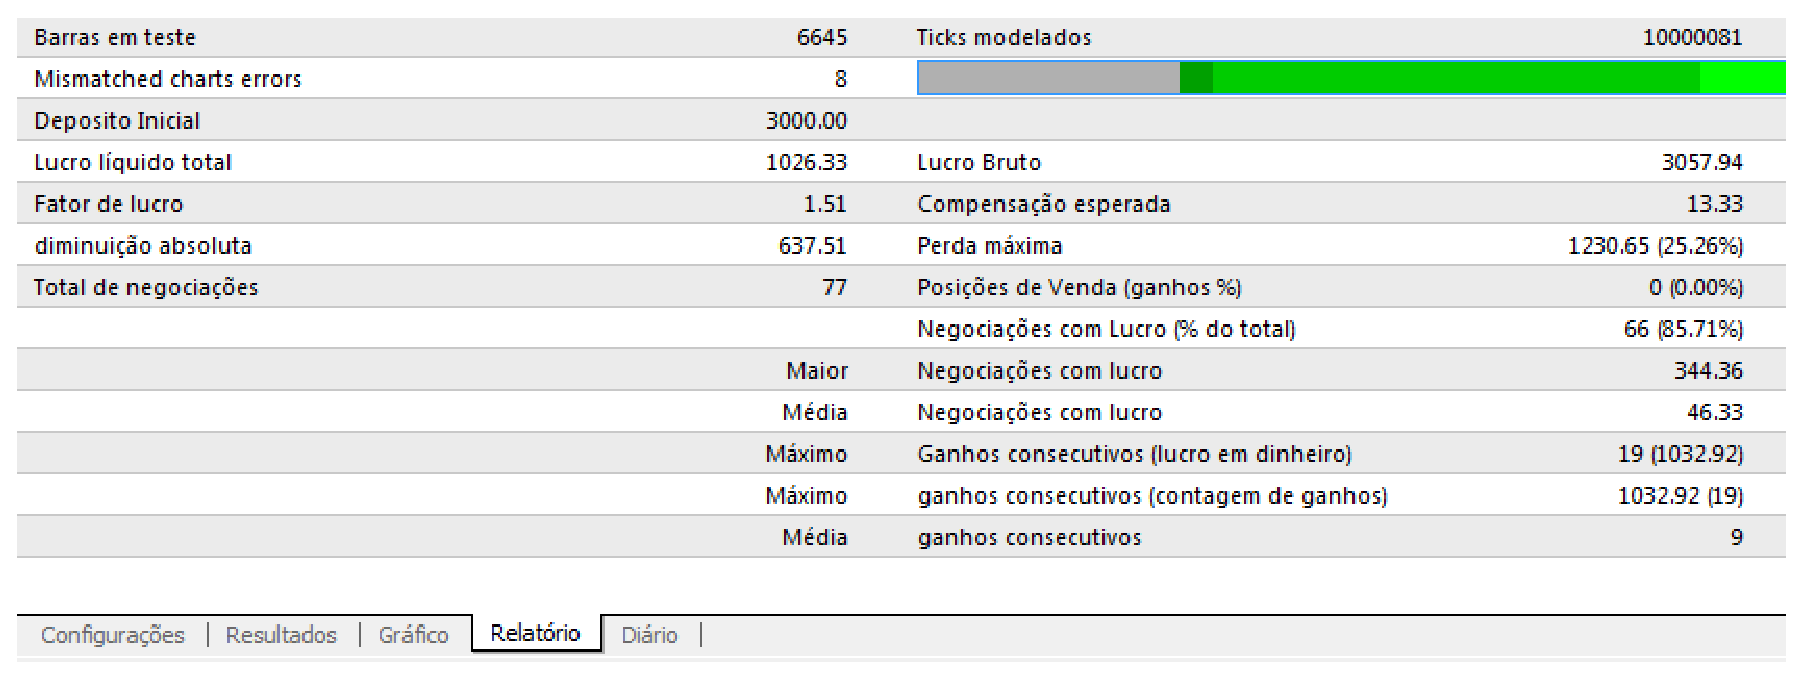
\includegraphics[width=0.9\textwidth]{figuras/protocoloMinimos2}
\caption{Relatório de simulação no período de Agosto de 2012 a Agosto de 2013 do \textit{expert} MinimosQuadrados.mql}
\label{protocoloMinimos2}
\end{figure}

O \textit{expert} MinimosQuadrados.mql, teve altos e baixos nas simulações durante os dois anos (2012 a 2013 e 2013 a 2014). Mas, no desempenho geral, conforme é evidenciado nos gráficos das Figuras \ref{protocoloMinimos3} e \ref{protocoloMinimos4}, o \textit{expert} teve um lucro acima de 10\% do capital inicial.

\newpage
\begin{figure}[H]
\centering
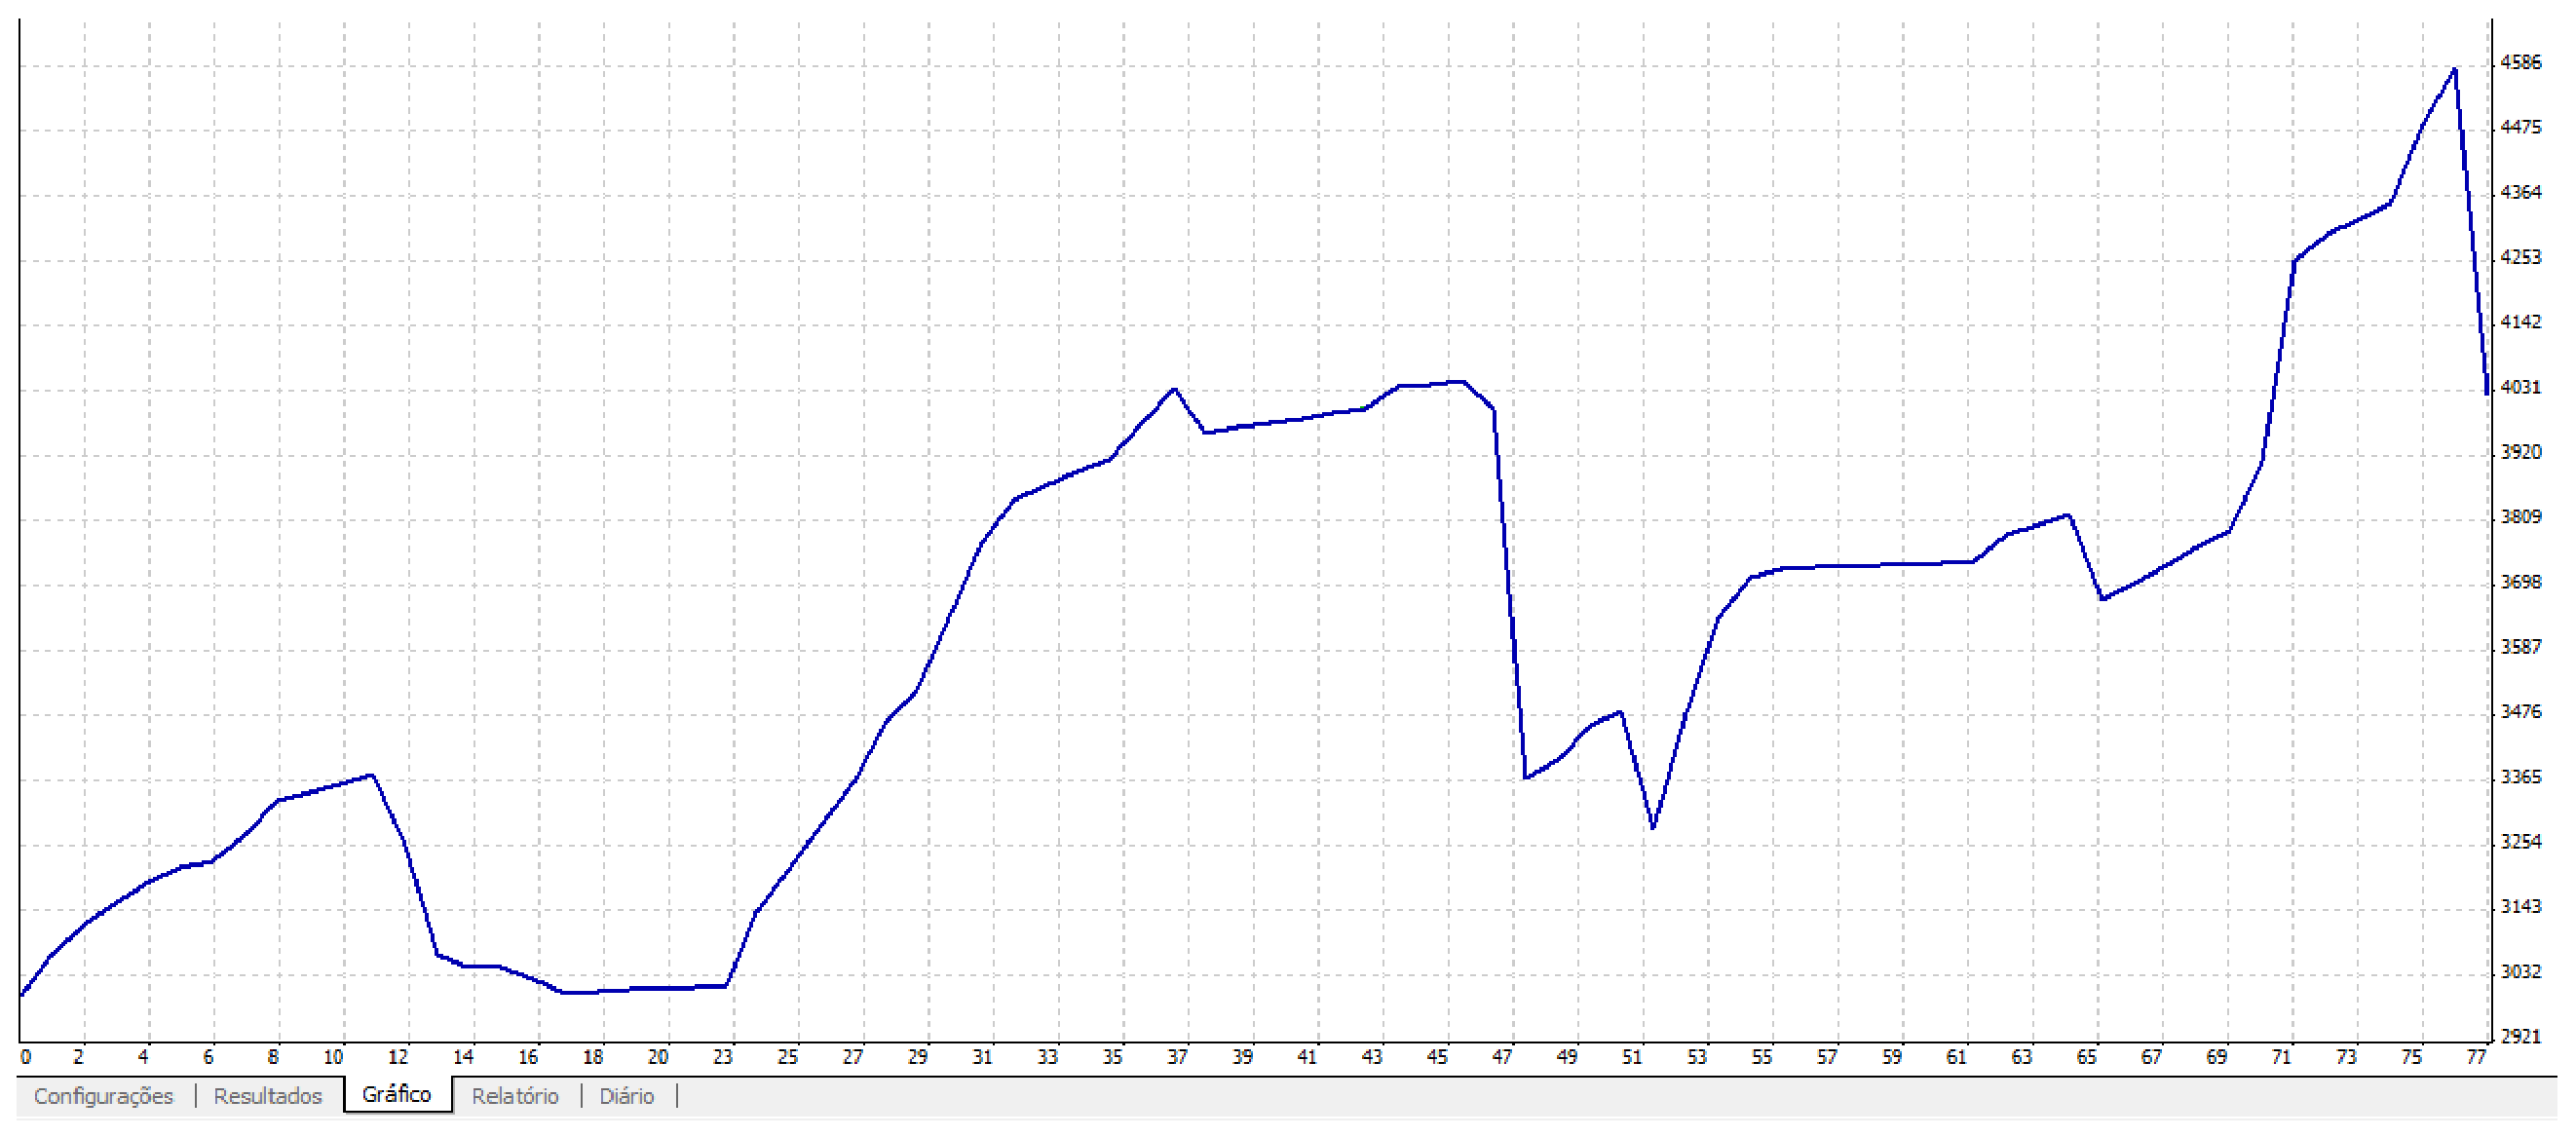
\includegraphics[width=0.9\textwidth]{figuras/protocoloMinimos3}
\caption{Gráfico gerado pela simulação do \textit{expert} MinimosQuadrados.mql no período de Agosto de 2012 a Agosto de 2013}
\label{protocoloMinimos3}
\end{figure}

\begin{figure}[H]
\centering
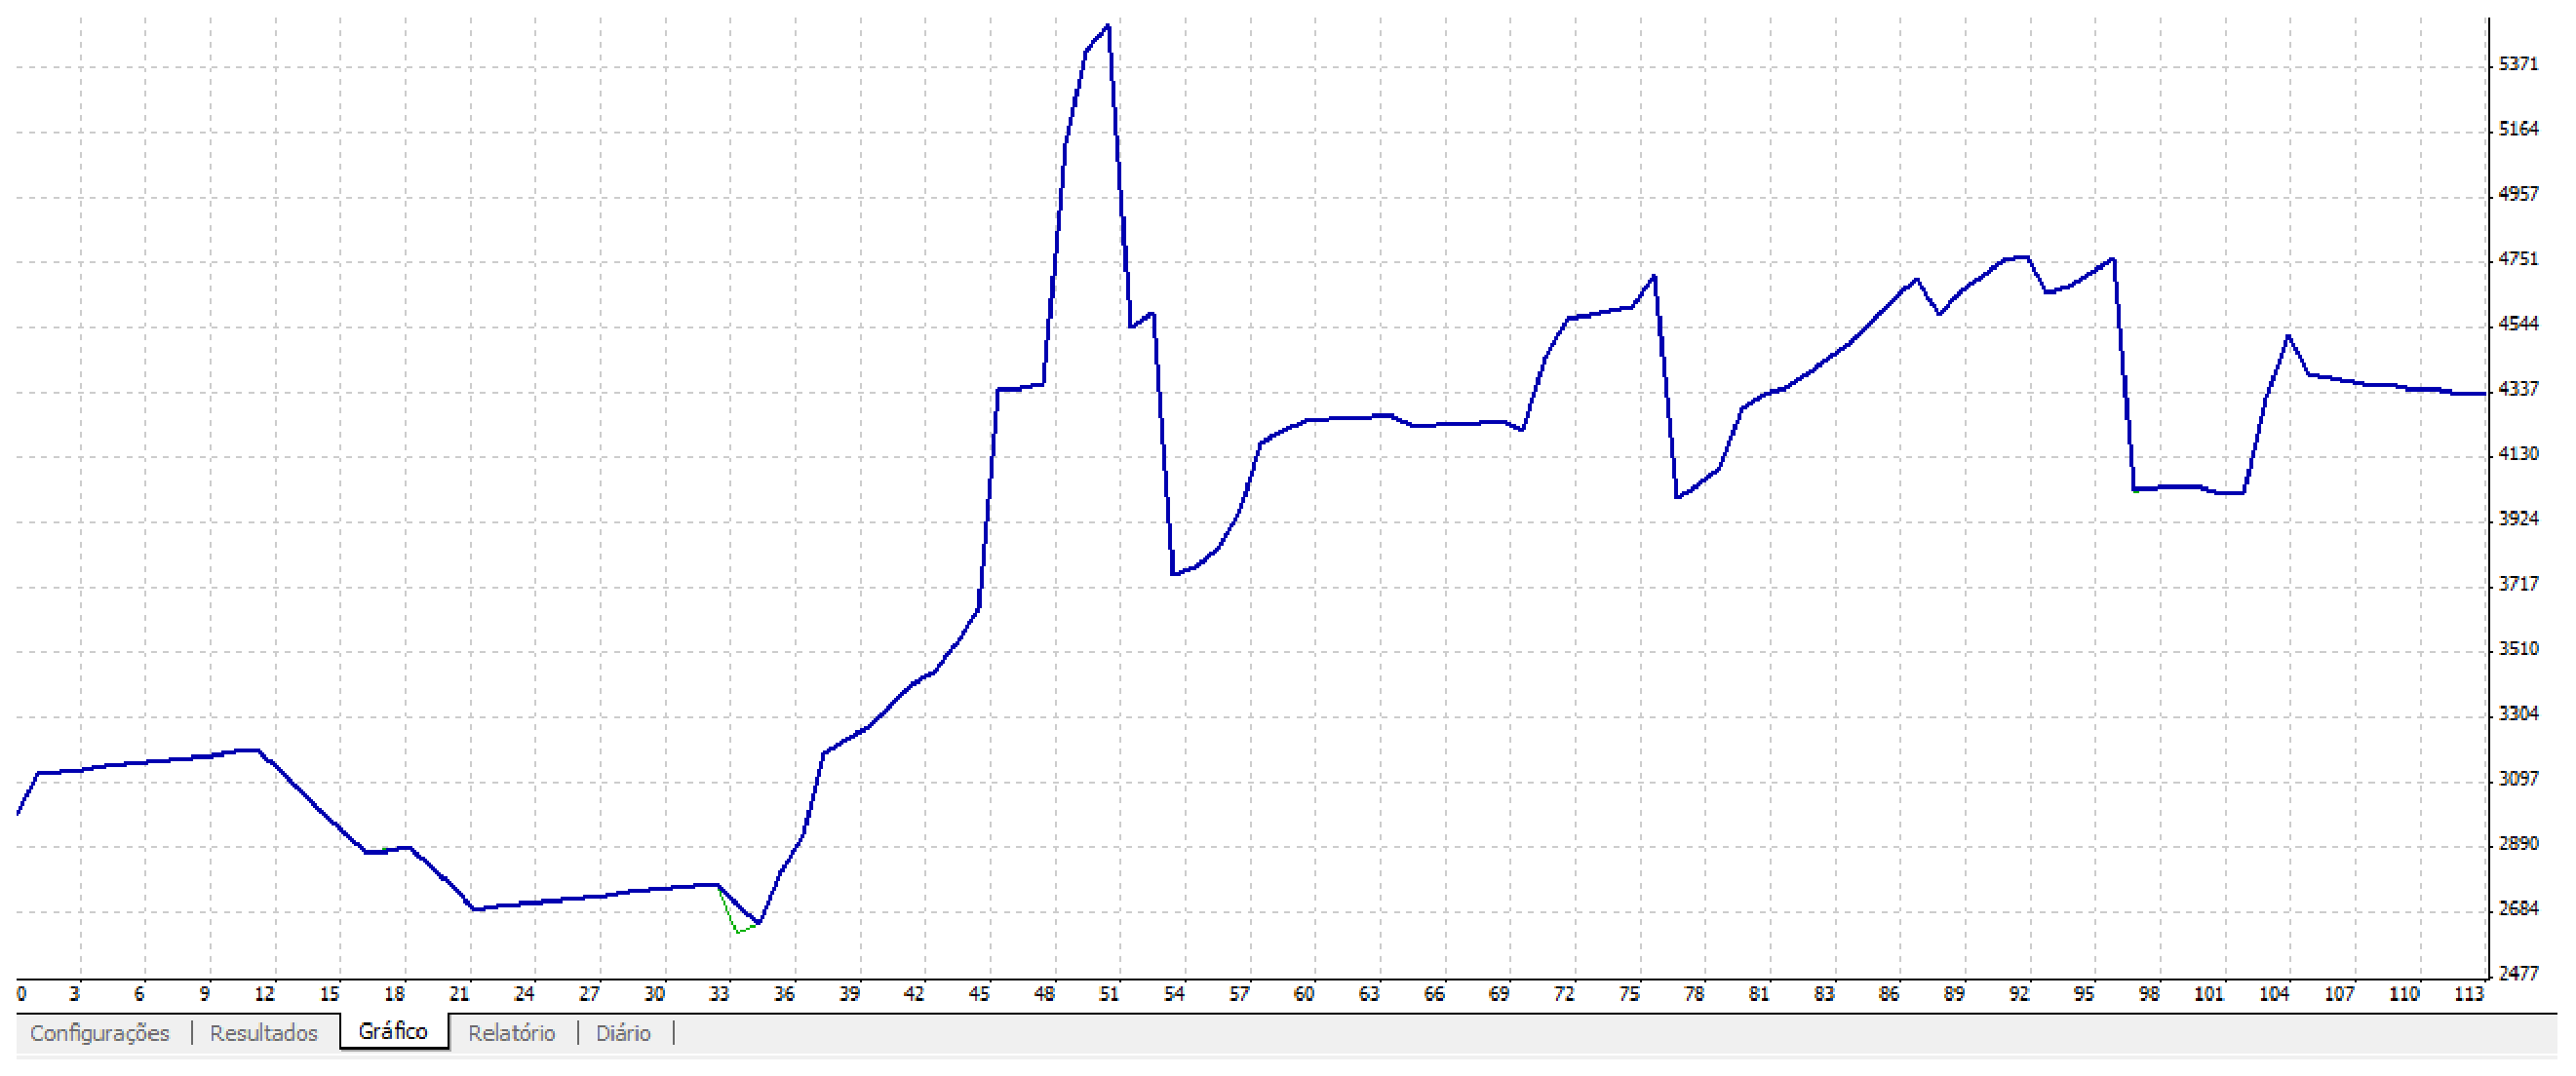
\includegraphics[width=0.9\textwidth]{figuras/protocoloMinimos4}
\caption{Gráfico gerado pela simulação do \textit{expert} MinimosQuadrados.mql no período de Agosto de 2013 a Agosto de 2014}
\label{protocoloMinimos4}
\end{figure}

\subsection{Simulação do método de Fibonacci}

O \textit{expert} Fibonacci.mql obteve o percentual de negociações com lucros de 72.73\% no período de Agosto de 2012 a Agosto de 2013, e o  lucro nesse período foi de 341.20 USD.
No período de Agosto de 2013 a Agosto de 2014, o percentual de negociações com lucros foi de 56.00\%,  e obteve-se o lucro de 659.05 USD. Apesar do percentual de acerto nesse período ter sido menor quando comparado ao período de agosto 2012-2013, o lucro obtido foi 51.77\% maior. Isso se deve ao fato do \textit{expert} ter negociado mais vezes (25 nesse período contra 11 no anterior) no período de Agosto 2013-2014.

Os relatórios completos das simulações podem ser visualizados nas Figuras \ref{protocoloFib} e \ref{protocoloFib2}.

\begin{figure}[H]
\centering
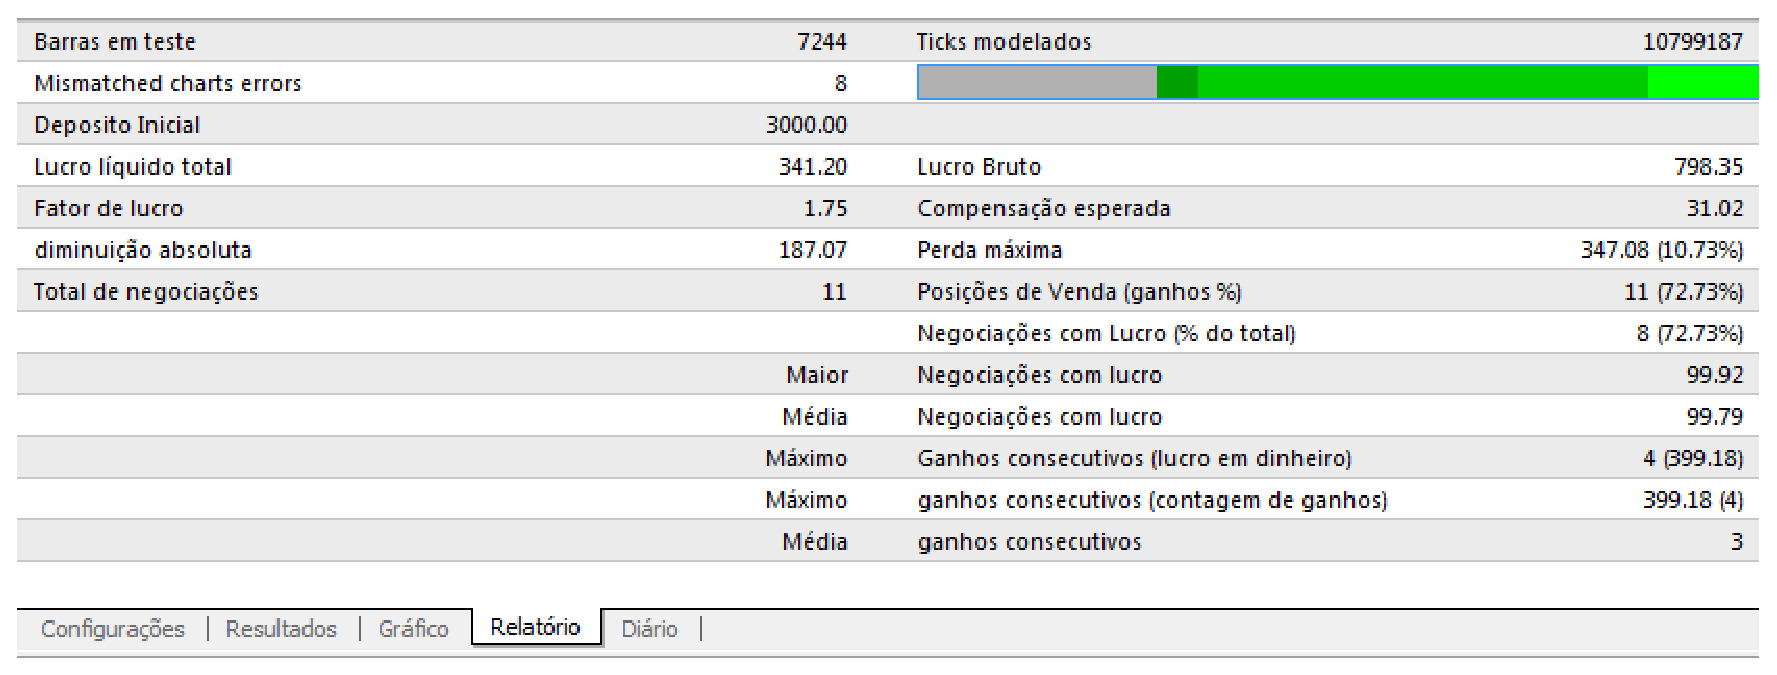
\includegraphics[width=0.9\textwidth]{figuras/protocoloFib}
\caption{Relatório de simulação no período de Agosto de 2012 s Agosto de 2013 do \textit{expert} Fibonacci.mql}
\label{protocoloFib}
\end{figure}

\begin{figure}[H]
\centering
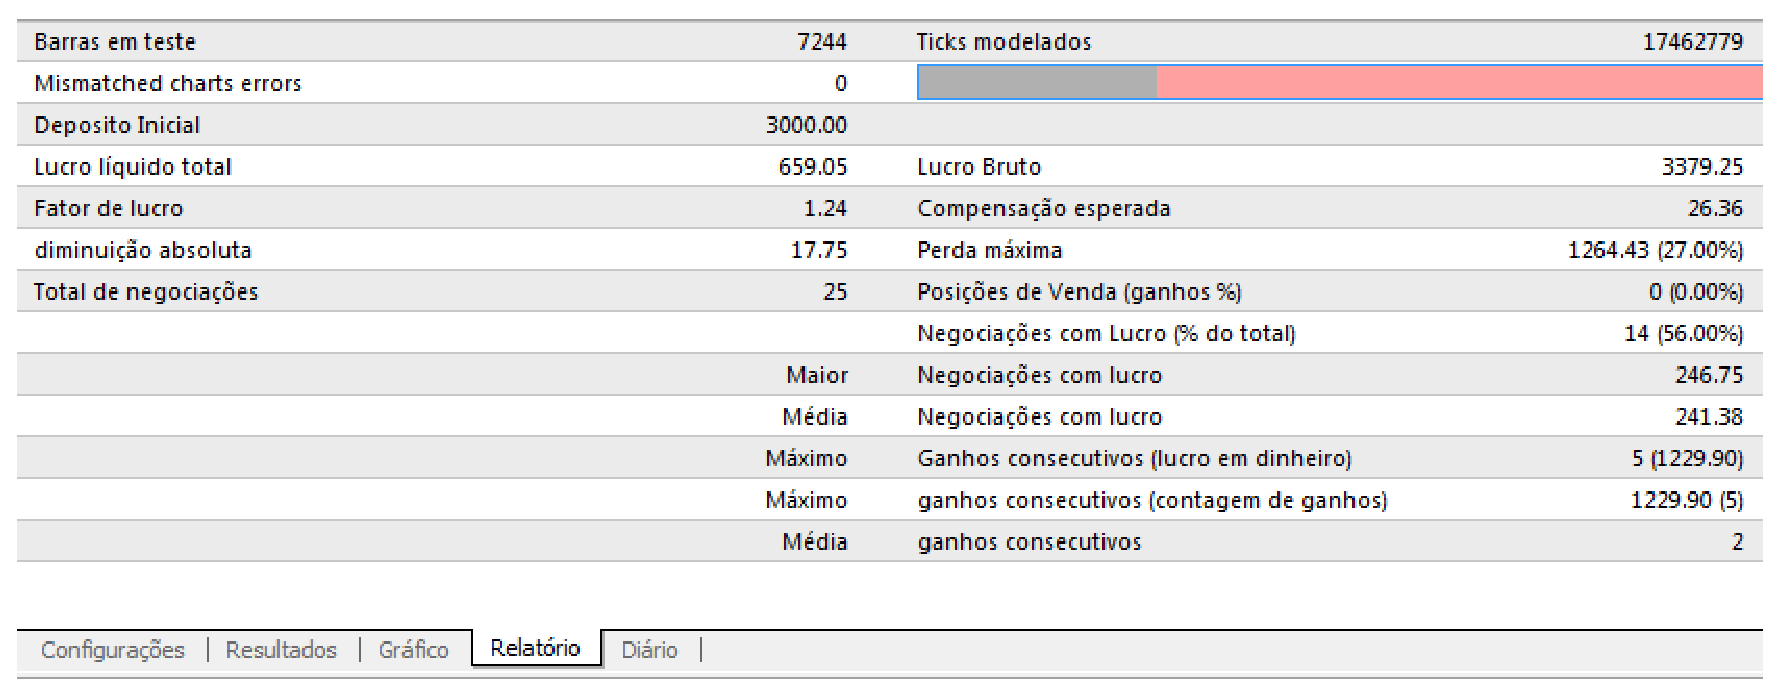
\includegraphics[width=0.9\textwidth]{figuras/protocoloFib2}
\caption{Relatório de simulação no período agosto 2013-2014 do \textit{expert} Fibonacci.mql}
\label{protocoloFib2}
\end{figure}

É possível visualizar nos gráficos das simulações os lucros de capital que o \textit{expert} Fibonacci.mql gerou, conforme ilustrado nas Figuras \ref{protocoloFib3} e \ref{protocoloFib4}.

\begin{figure}[H]
\centering
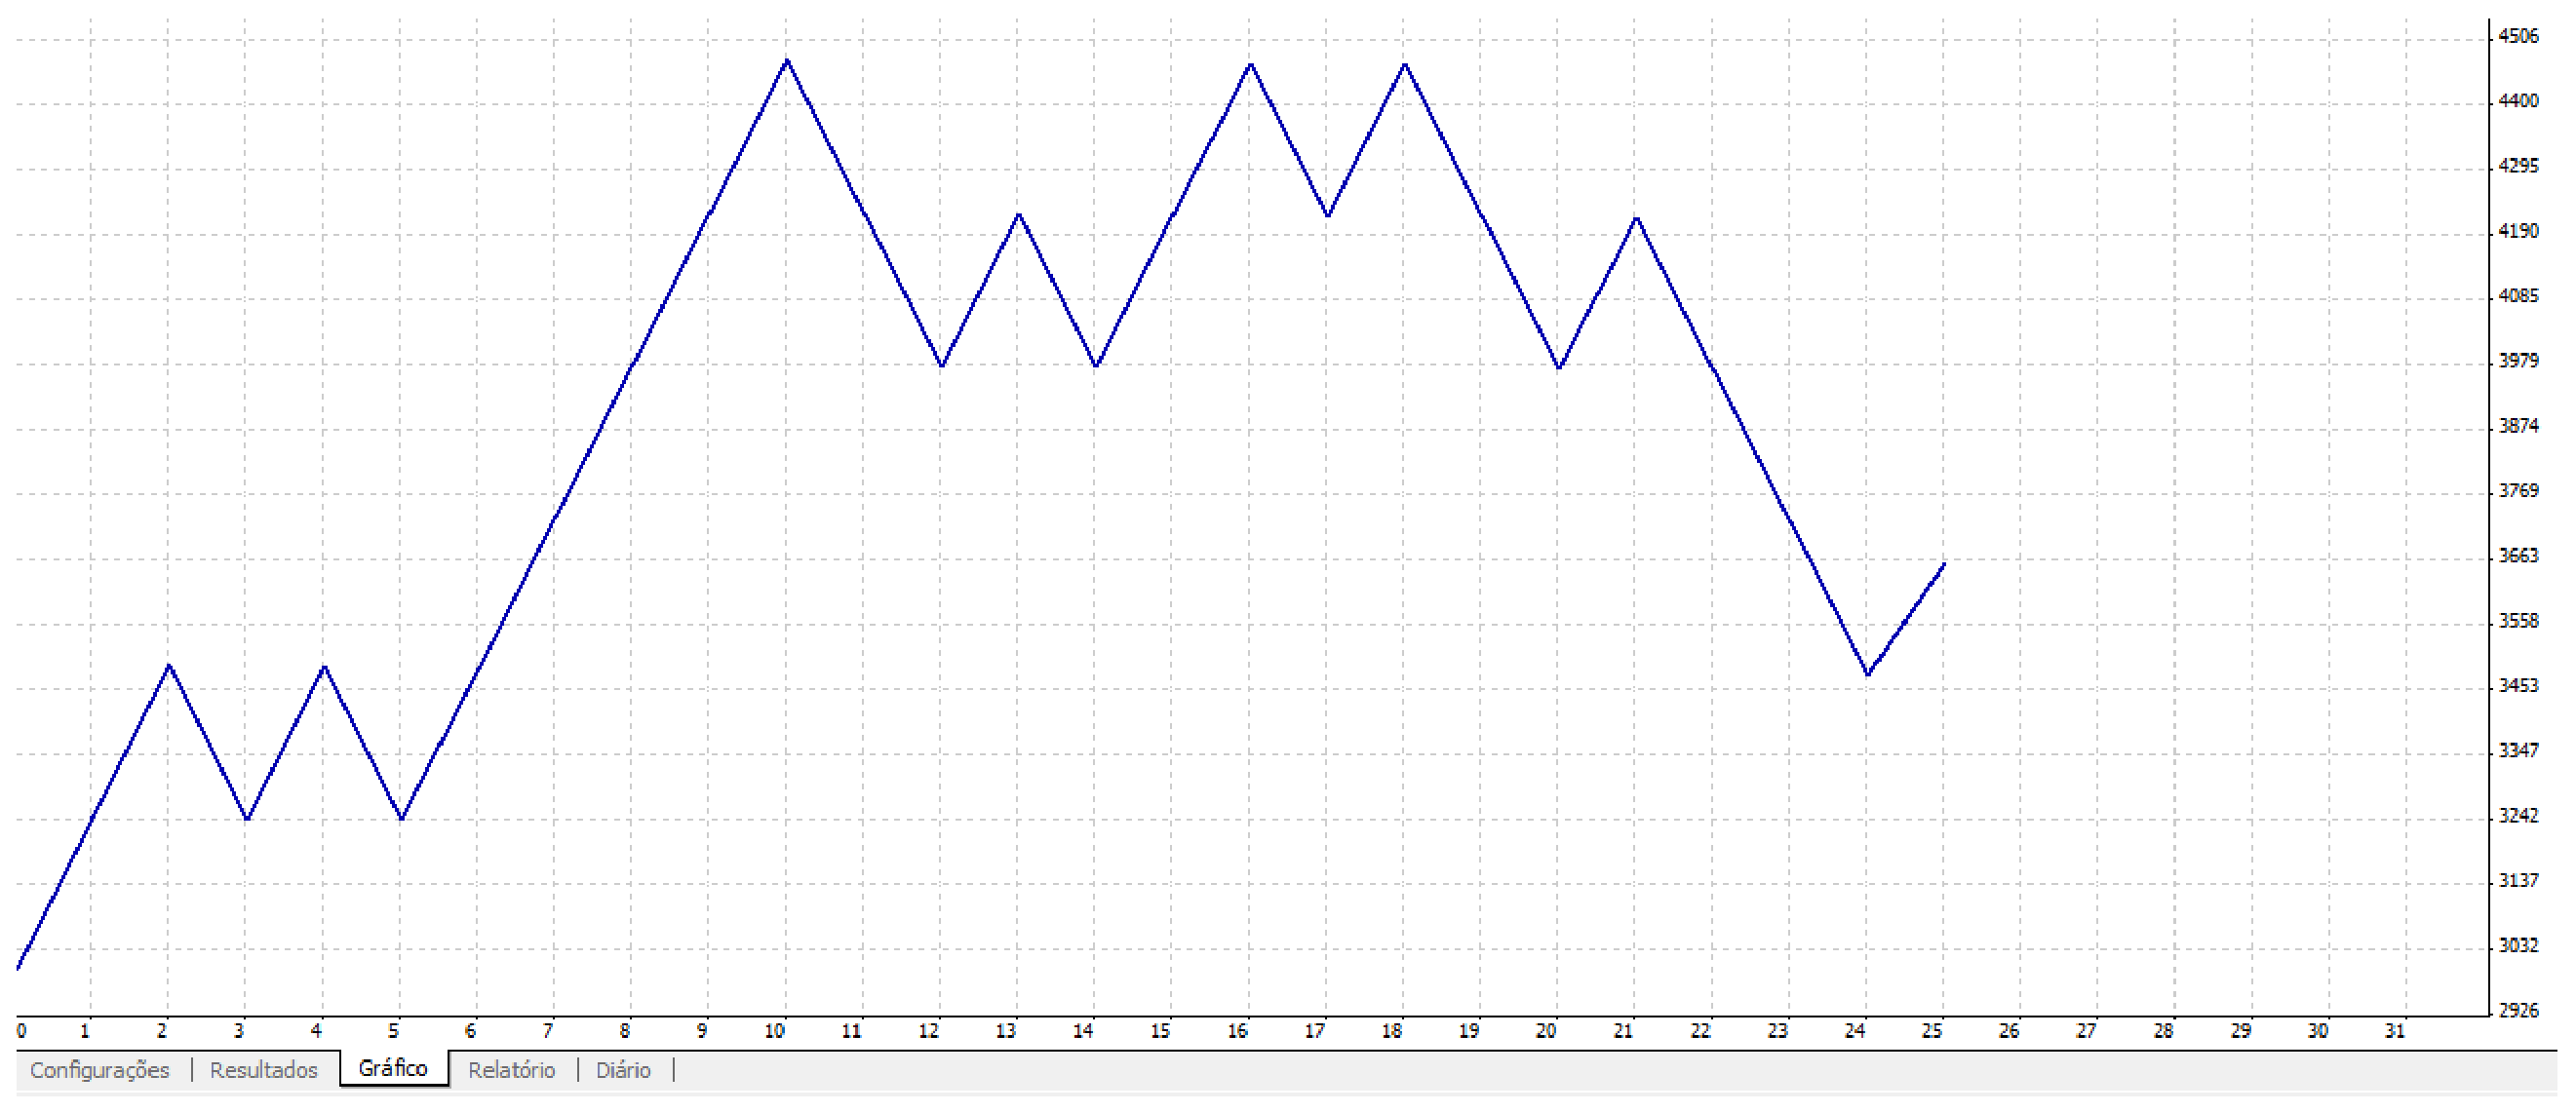
\includegraphics[width=0.9\textwidth]{figuras/protocoloFib3}
\caption{Gráfico gerado pela simulação do \textit{expert} Fibonacci.mql no período de Agosto de 2012 a Agosto de 2013}
\label{protocoloFib3}
\end{figure}

\begin{figure}[H]
\centering
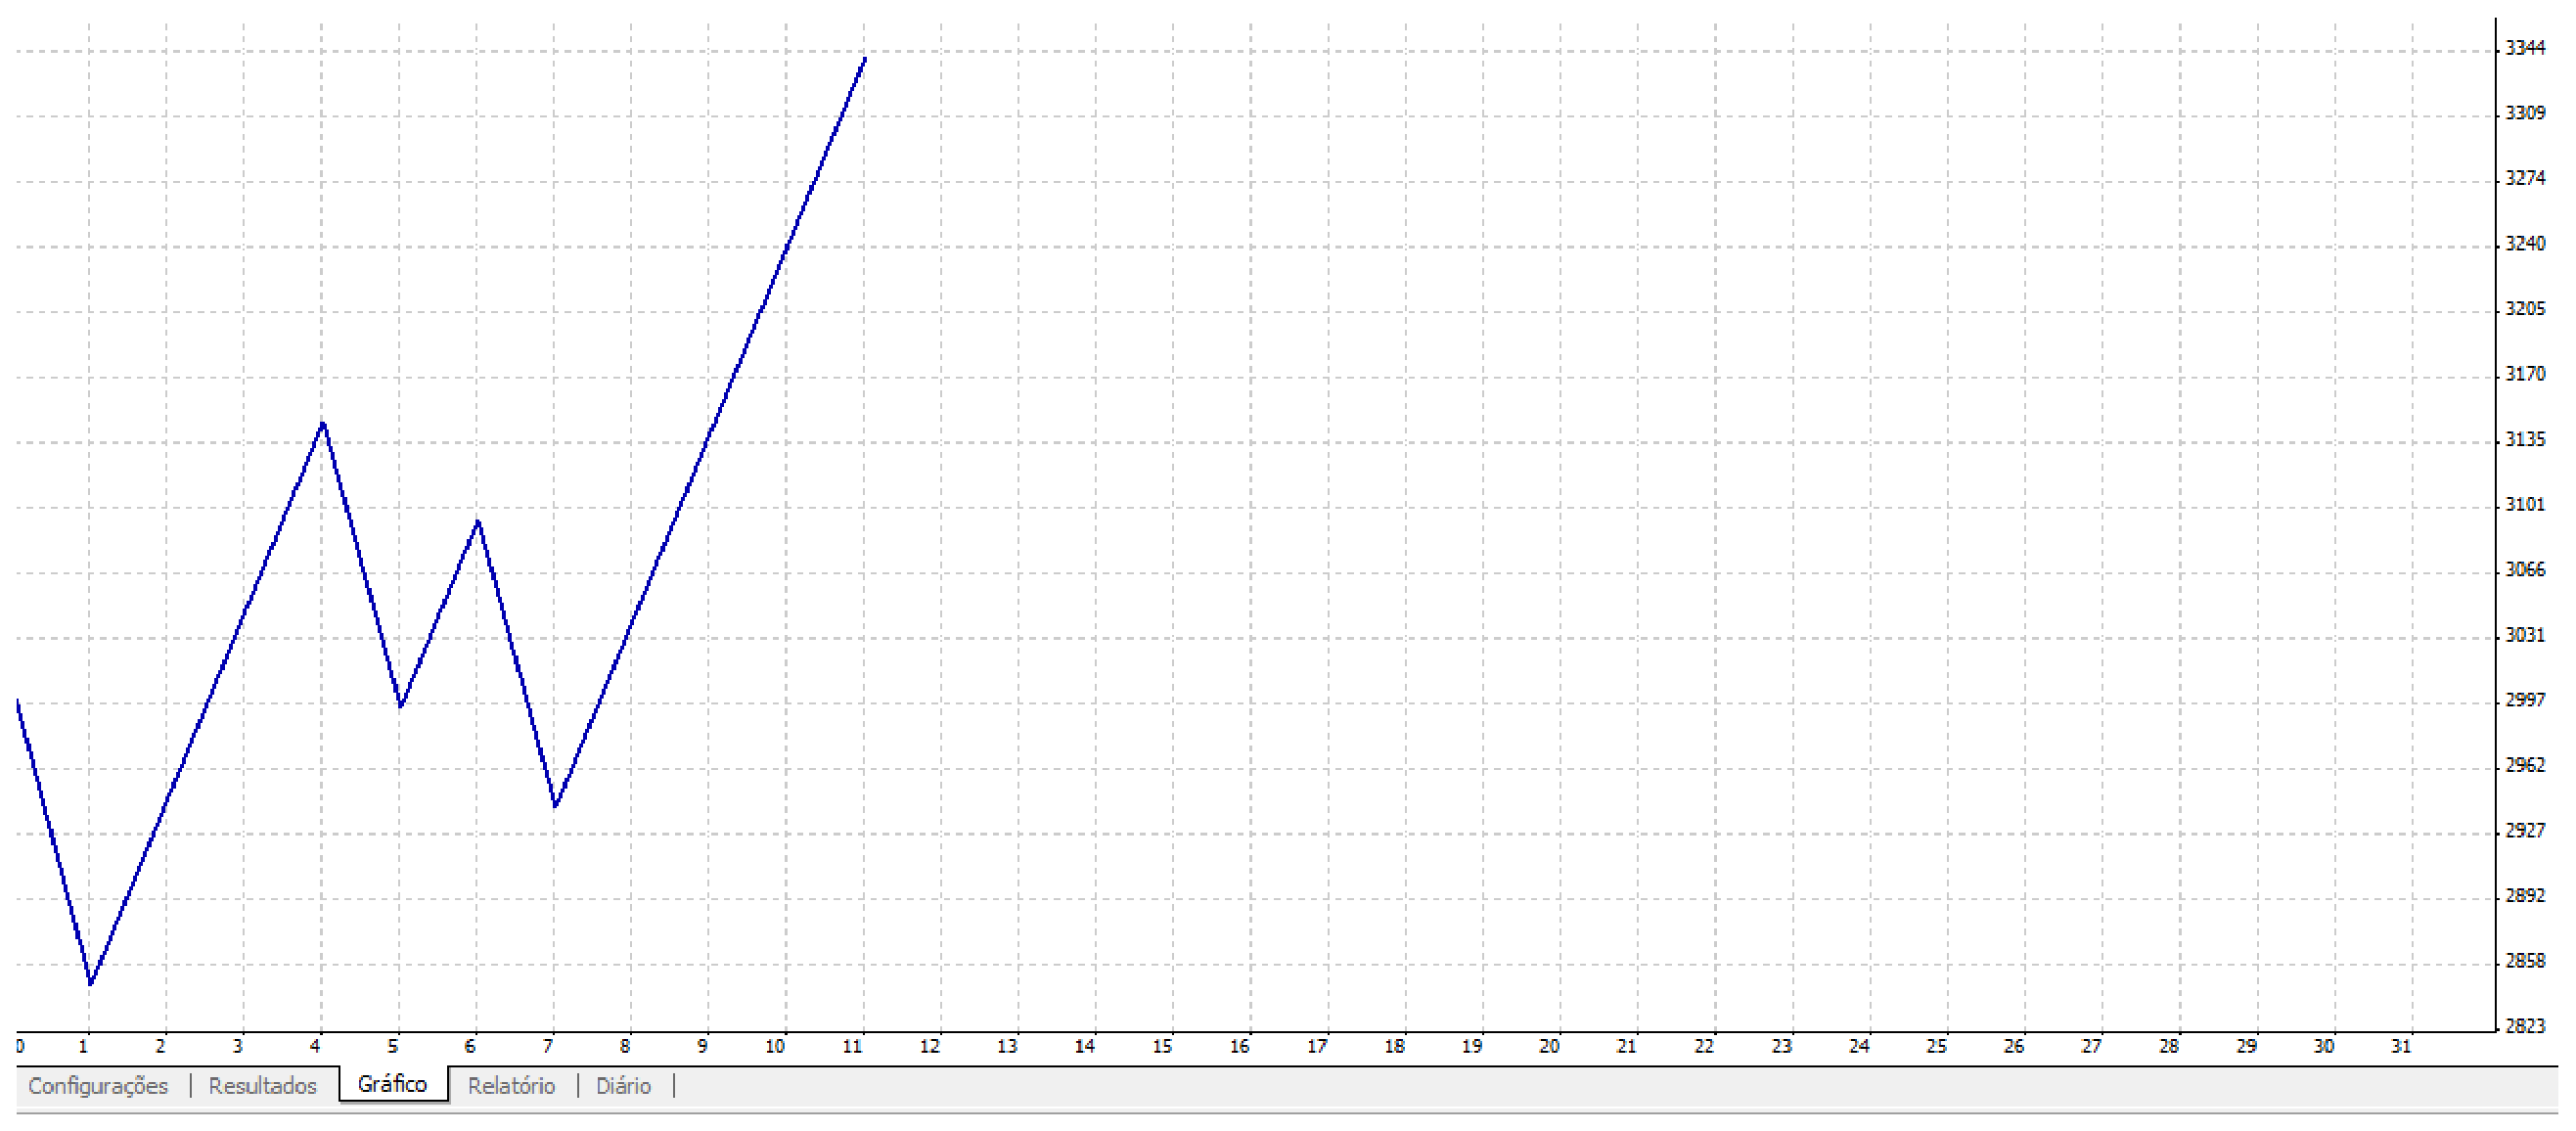
\includegraphics[width=0.9\textwidth]{figuras/protocoloFib4}
\caption{Gráfico gerado pela simulação do \textit{expert} Fibonacci.mql no período de Agosto de 2013 a Agosto de 2014}
\label{protocoloFib4}
\end{figure}

\subsection{Simulação do método de Estocástico}

O \textit{expert} Estocastico.mql obteve o percentual de negociações com lucros de 47.47\% no período agosto 2012-2013. Portanto, o percentual de negociações com perdas foi de 52.53\%. Nesse período, o \textit{expert} teve um prejuízo de 1110.88 USD.

No período de Agosto de 2013 a Agosto de 2014, o percentual de negociações com lucros foi de 47.70\% (percentual com perdas de 52.30\%),  e obteve-se o prejuízo de 459.17 USD. 
Os relatórios completos das simulações podem ser visualizados nas Figuras \ref{protocoloEst} e \ref{protocoloEst2}.

\begin{figure}[H]
\centering
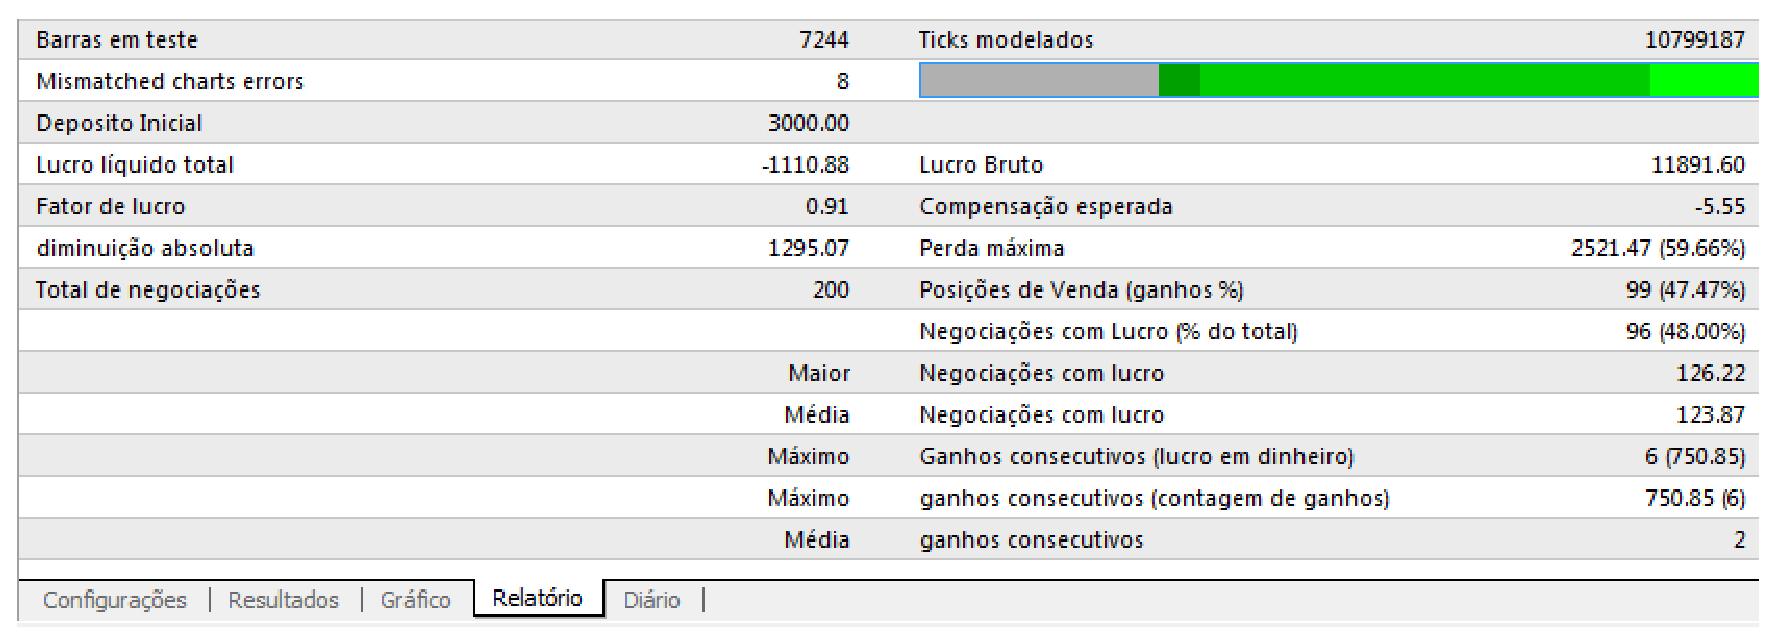
\includegraphics[width=0.9\textwidth]{figuras/protocoloEst}
\caption{Relatório de simulação no período de Agosto de 2012 a Agosto de 2013 do \textit{expert} Estocastico.mql}
\label{protocoloEst}
\end{figure}

\newpage
\begin{figure}[H]
\centering
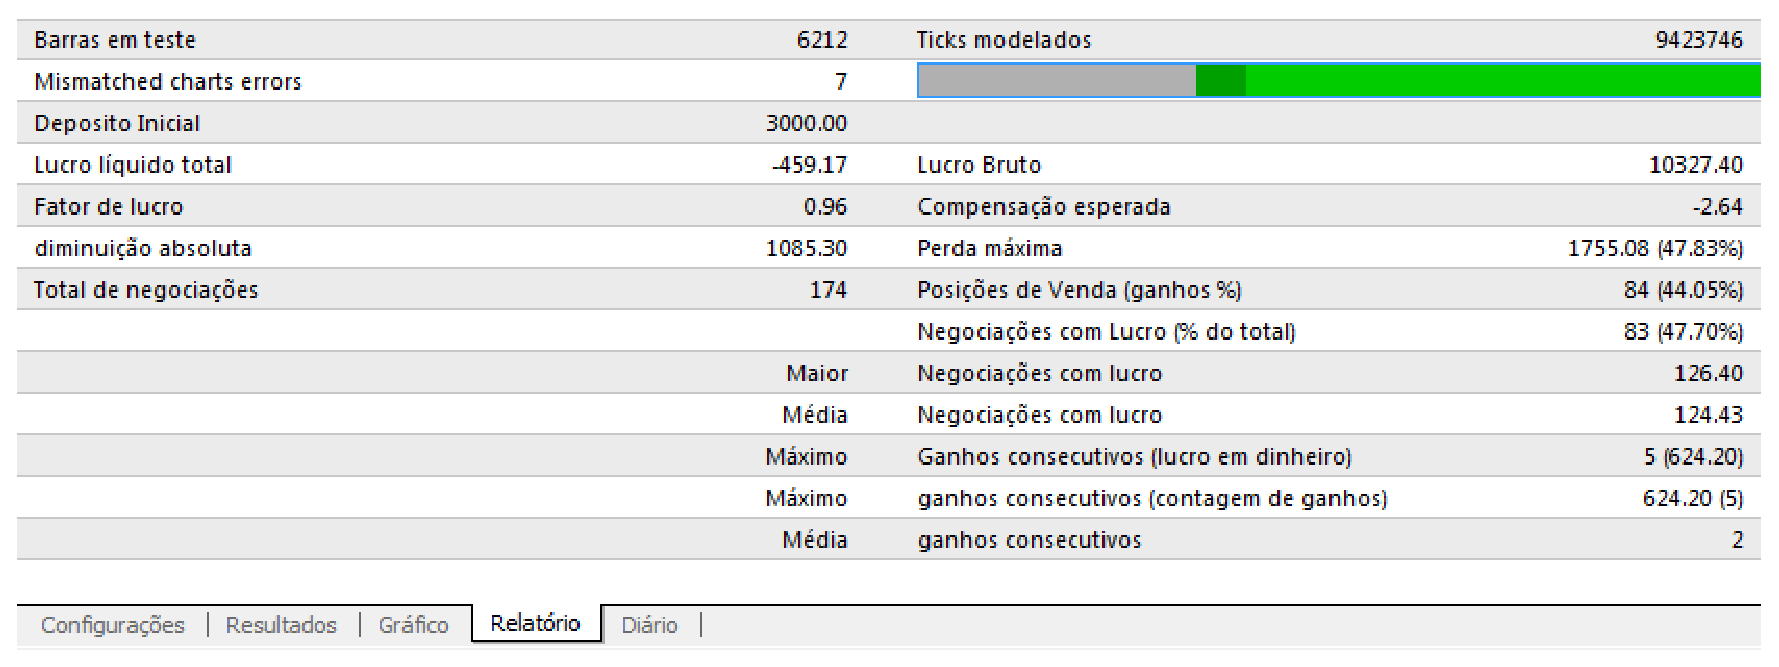
\includegraphics[width=0.9\textwidth]{figuras/protocoloEst2}
\caption{Relatório de simulação no período de Agosto de 2013 a Agosto de 2014 do \textit{expert} Estocastico.mql}
\label{protocoloEst2}
\end{figure}

É possível visualizar nos gráficos das simulações, as perdas de capital que o \textit{expert} Estocastico.mql gerou, confome ilustrado nas Figuras \ref{protocoloEst3} e \ref{protocoloEst4}.

\begin{figure}[H]
\centering
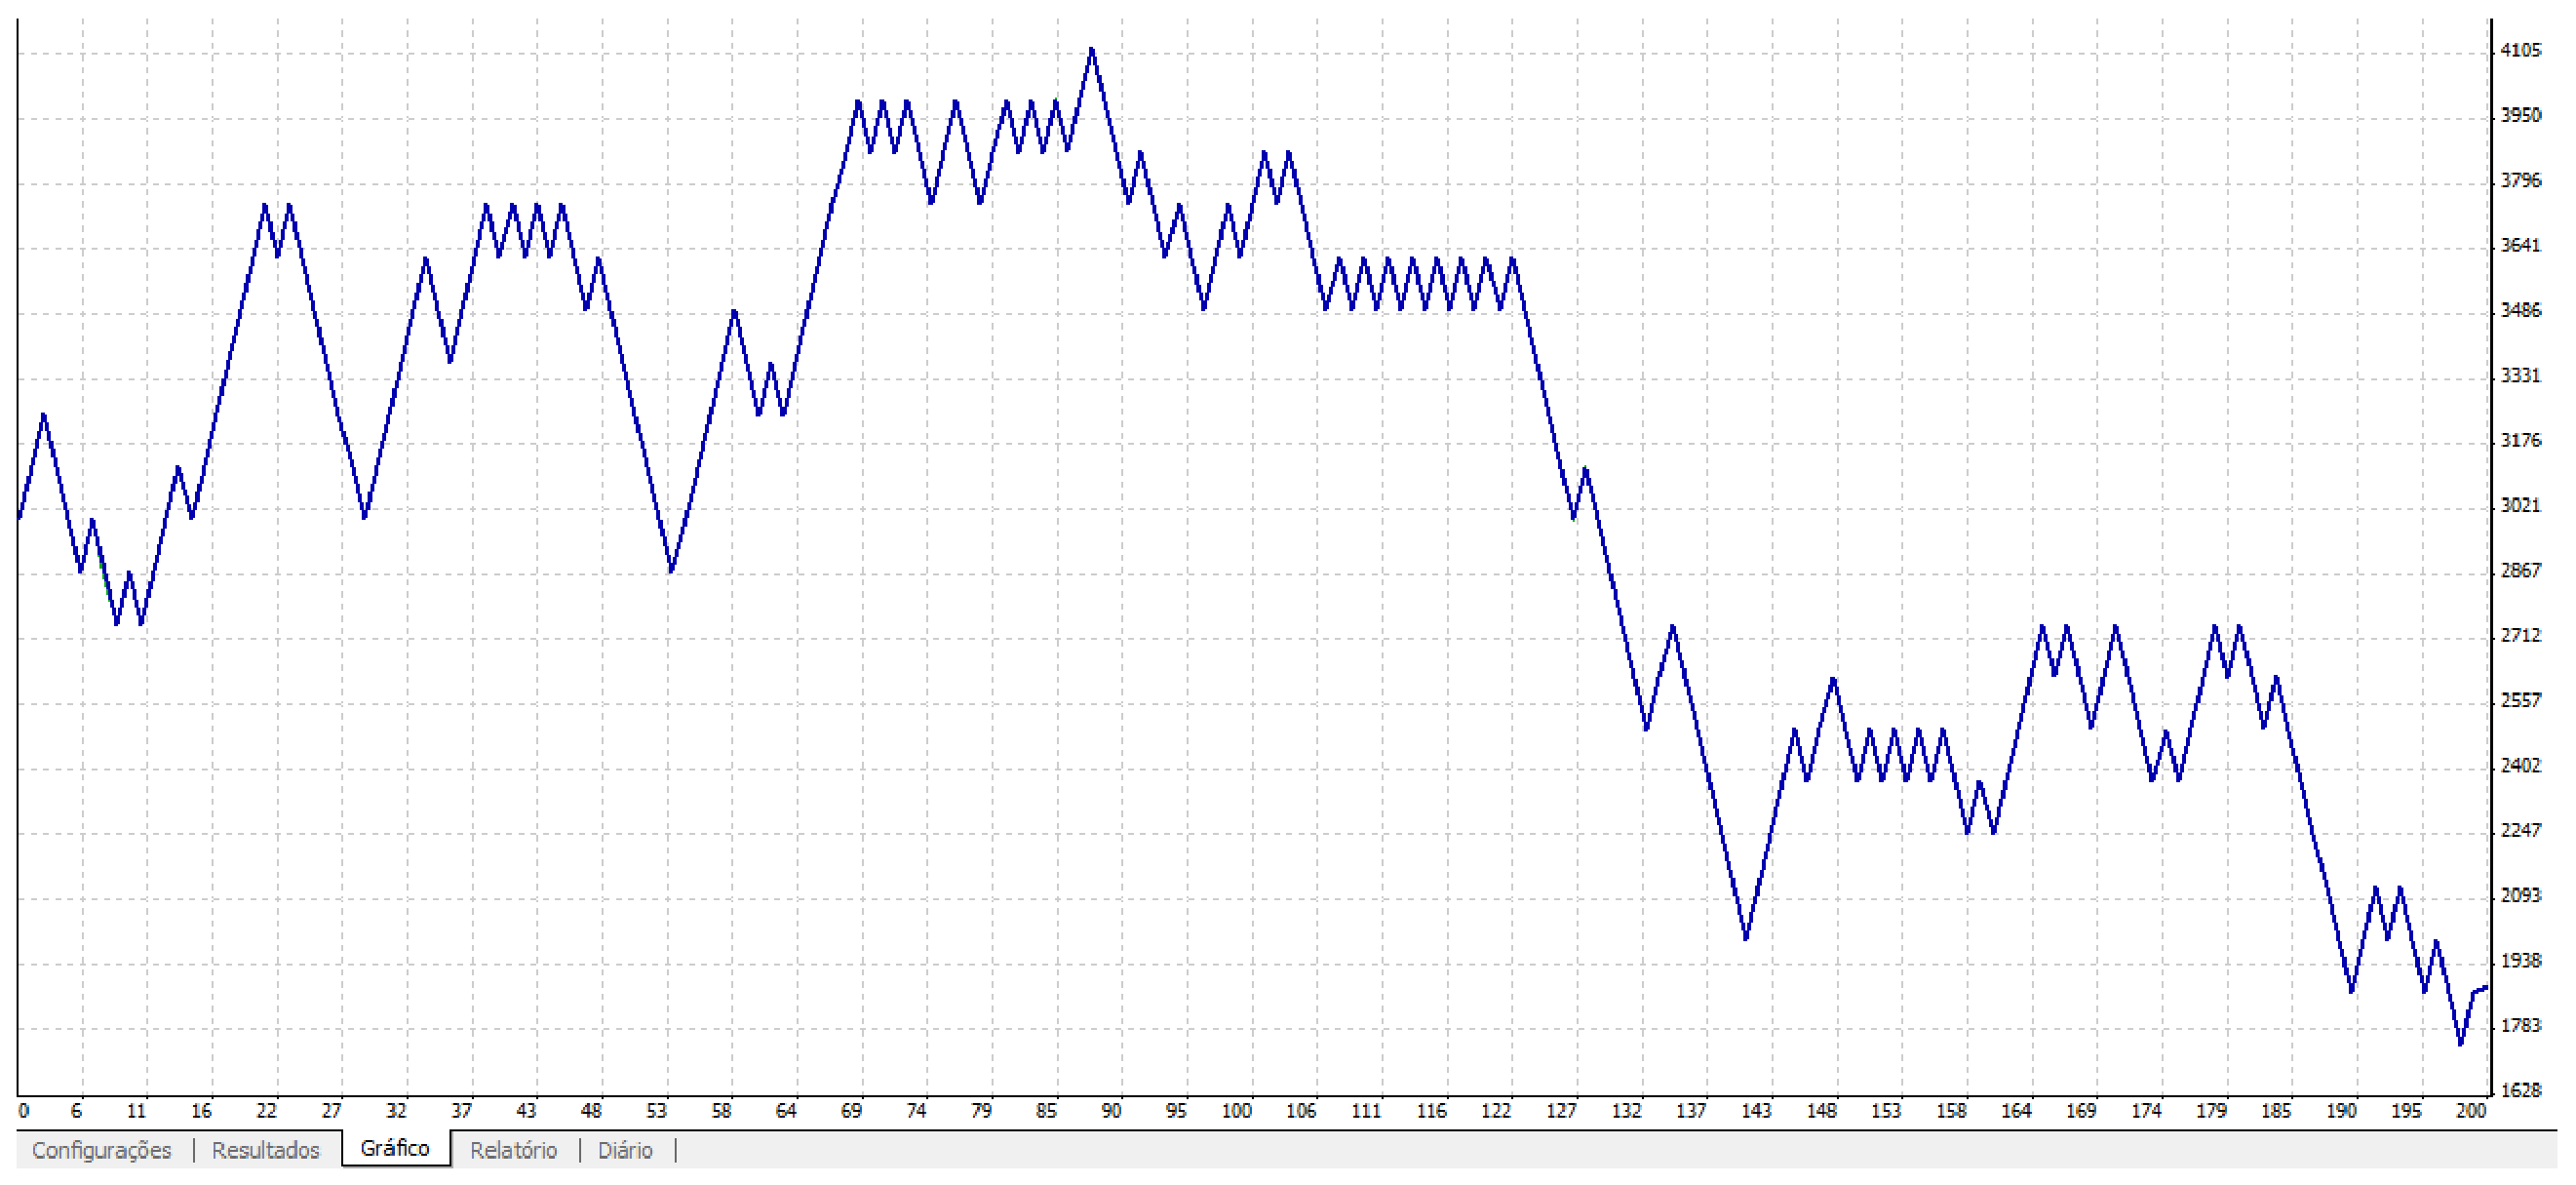
\includegraphics[width=0.9\textwidth]{figuras/protocoloEst3}
\caption{Gráfico gerado pela simulação do \textit{expert} Estocastico.mql no período de Agosto de 2012 a Agosto de 2013} 
\label{protocoloEst3}
\end{figure}

\newpage
\begin{figure}[H]
\centering
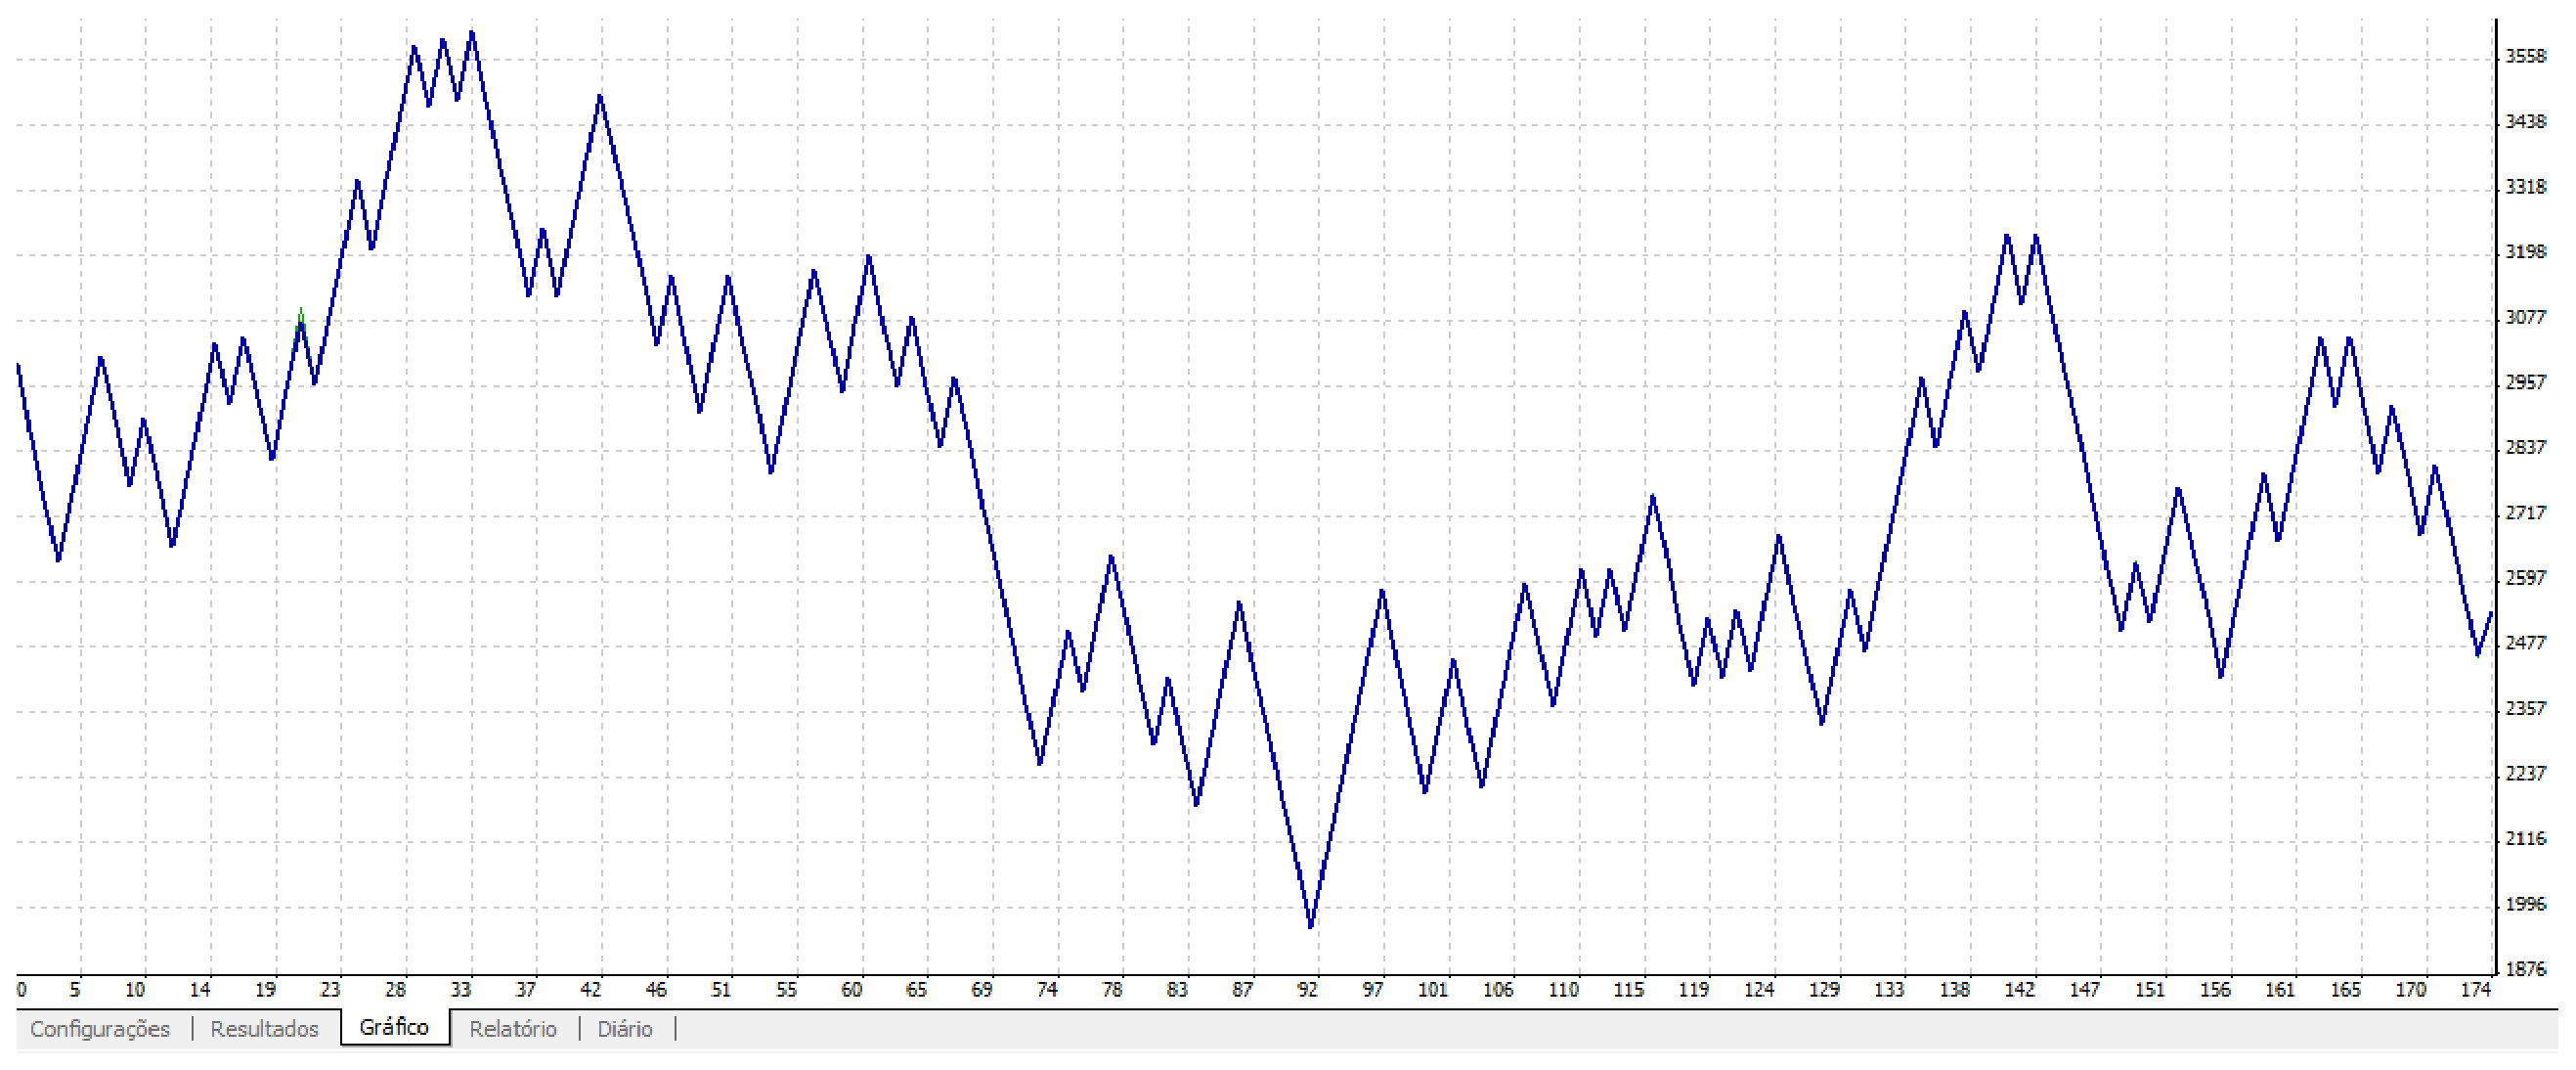
\includegraphics[width=0.9\textwidth]{figuras/protocoloEst4}
\caption{Gráfico gerado pela simulação do \textit{expert} Estocastico.mql no período de Agosto de 2013 a Agosto de 2014} 
\label{protocoloEst4}
\end{figure}

\subsection{Simulação do método de Média Móvel}

O \textit{expert} MediaMovel.mql obteve o percentual de negociações com lucros de 43.55\% no período de Agosto de 2012 a Agosto de 2013. Portanto, o percentual de negociações com perdas foi de 56.45\%. Nesse período, o \textit{expert} obteve um prejuízo de 2987.00 USD. 

No período de Agosto de 2013 a Agosto de  2014, o percentual de negociações com lucros foi de 48.48\%, e o percentual de negociação com prejuízos foi de 51.82\%.  Foi obtido um prejuízo de 459.17 USD. 

Os relatórios completos das simulações podem ser visualizados nas Figuras \ref{protocoloMedia} e \ref{protocoloMedia2}.

\begin{figure}[H]
\centering
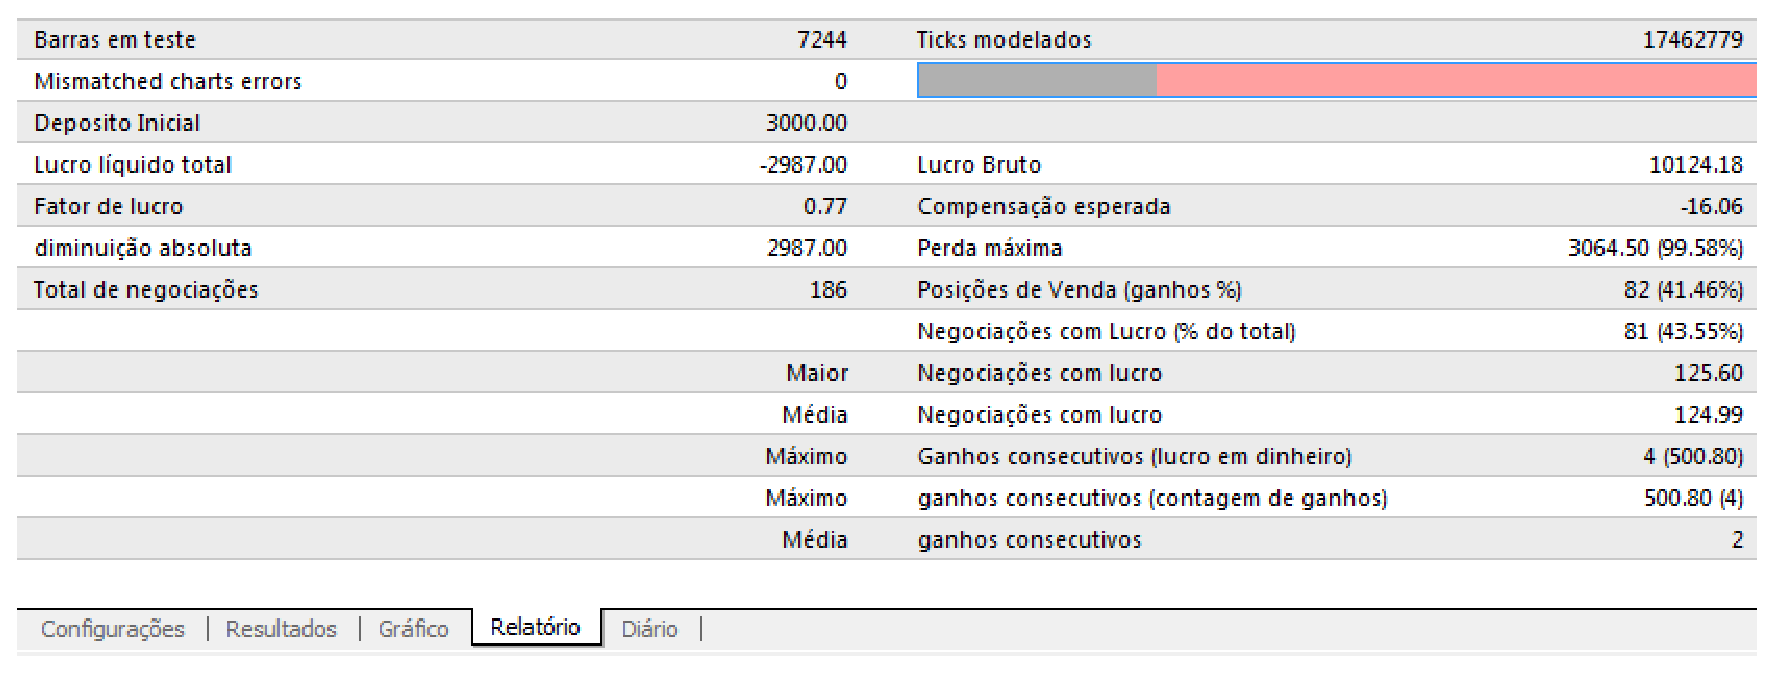
\includegraphics[width=0.9\textwidth]{figuras/protocoloMedia}
\caption{Relatório de simulação no período de Agosto de 2012 a Agosto de 2013 do \textit{expert} MediaMovel.mql} 
\label{protocoloMedia}
\end{figure}

\newpage
\begin{figure}[H]
\centering
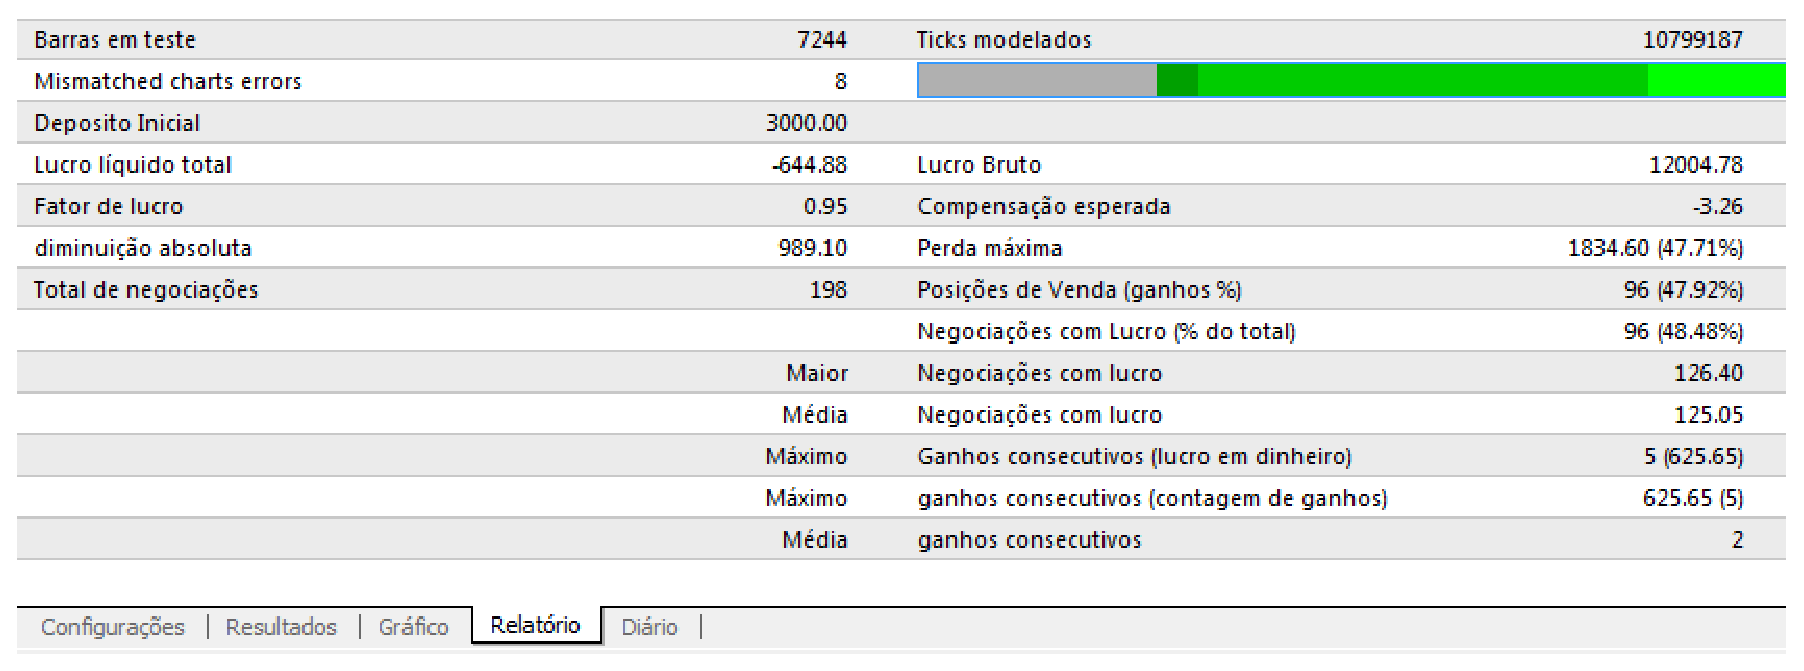
\includegraphics[width=0.9\textwidth]{figuras/protocoloMedia2}
\caption{Relatório de simulação no período de Agosto de 2013 a Agosto de 2014 do \textit{expert} MediaMovel.mql} 
\label{protocoloMedia2}
\end{figure}

É possível visualizar nos gráficos das simulações, as perdas de capital que o \textit{expert} MediaMovel.mql gerou, conforme ilustrado nas Figuras \ref{protocoloMedia3} e \ref{protocoloMedia4}.

\begin{figure}[H]
\centering
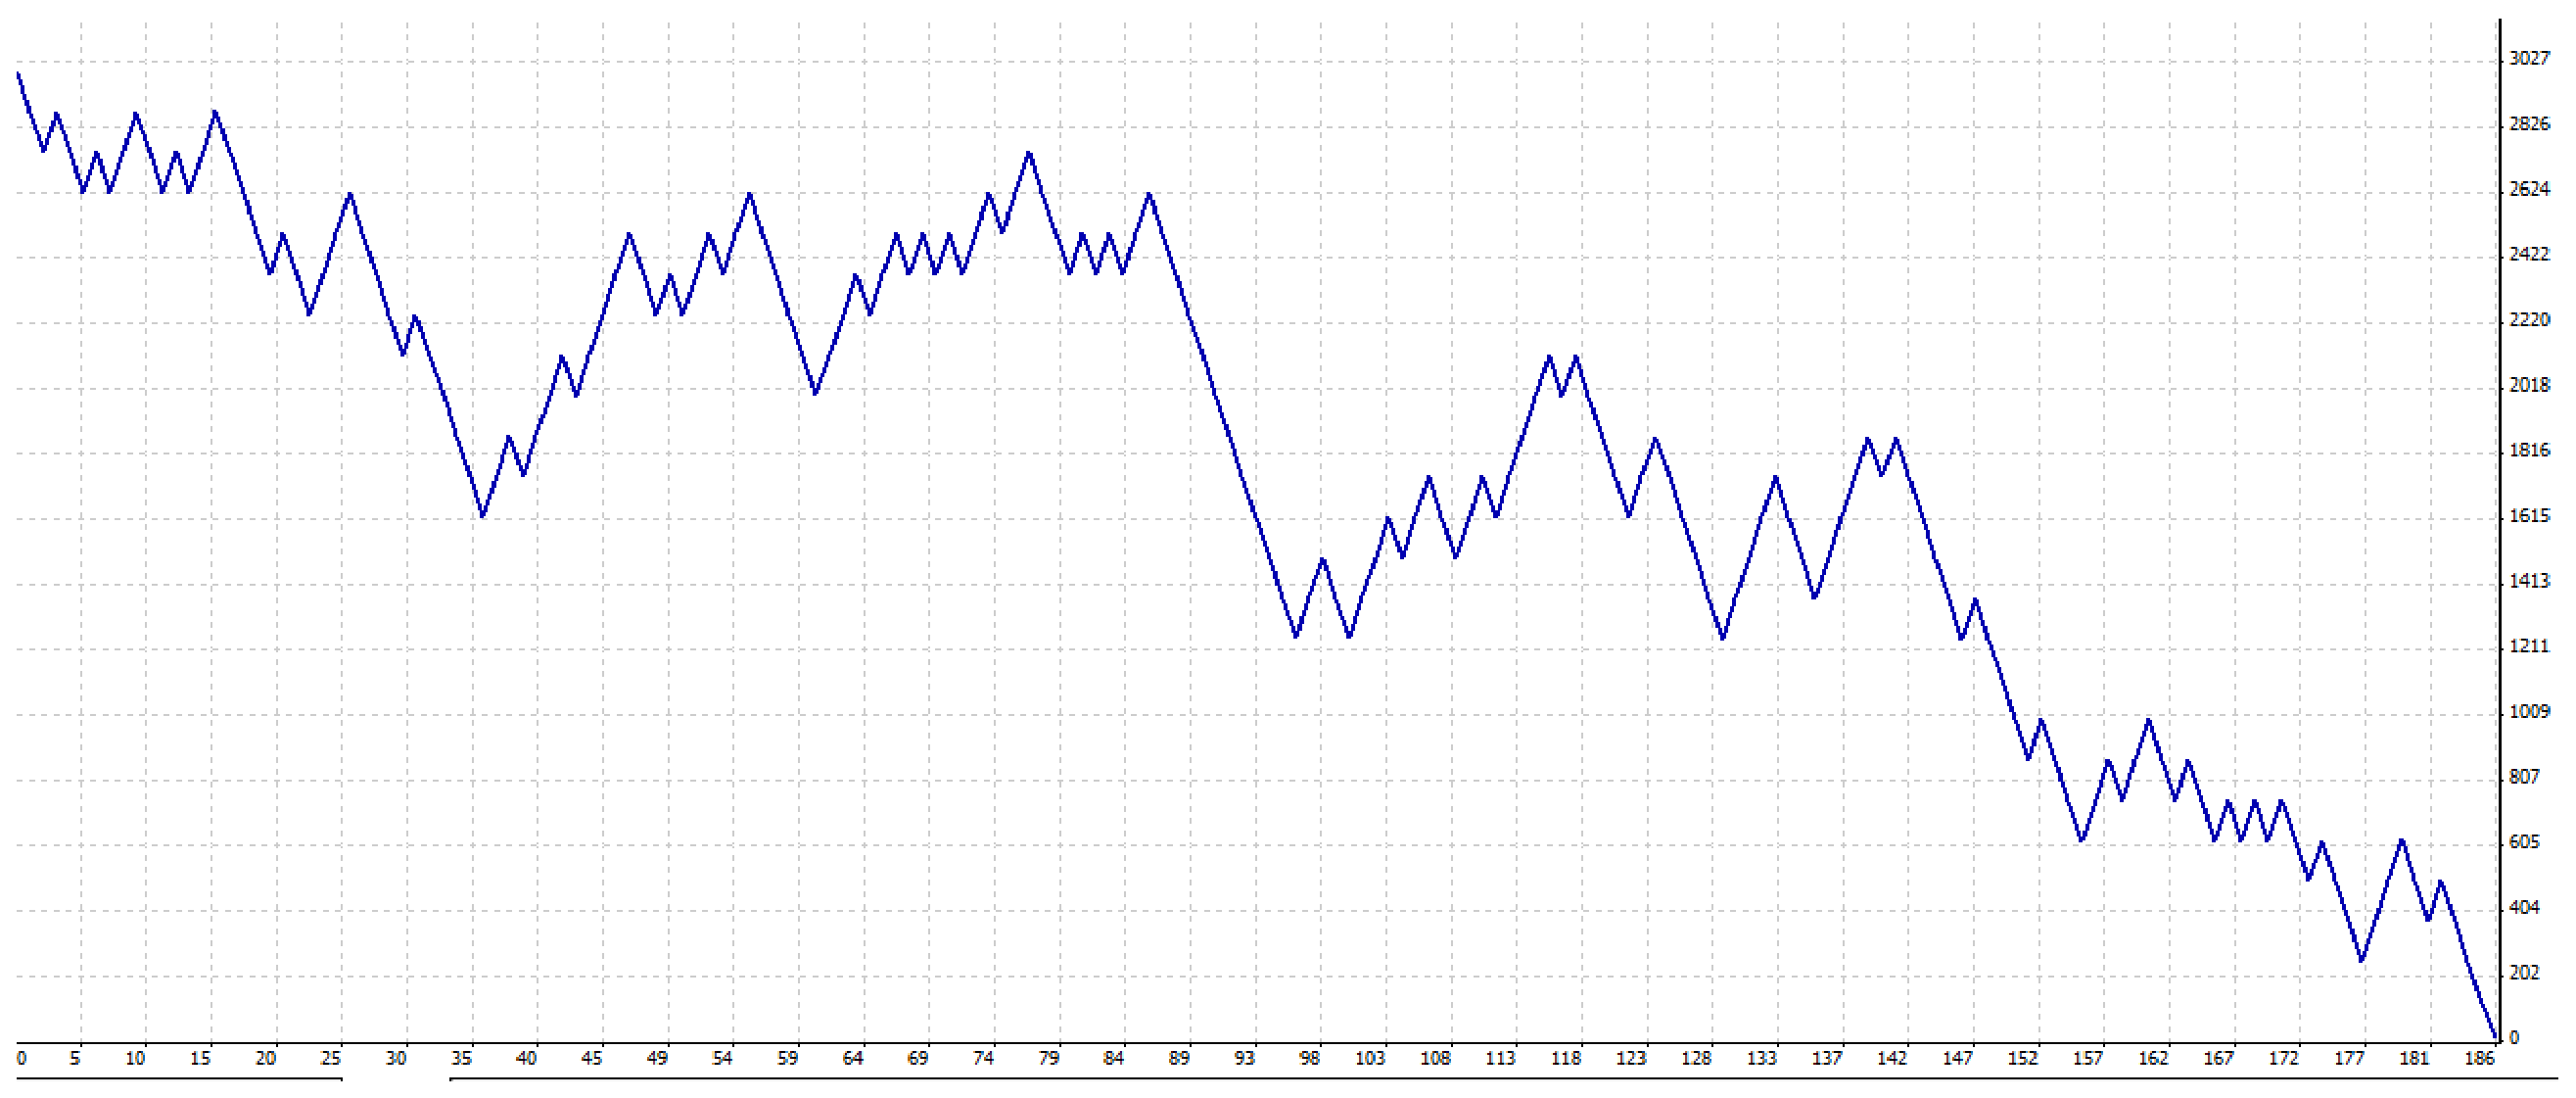
\includegraphics[width=0.9\textwidth]{figuras/protocoloMedia3}
\caption{ Gráfico gerado pela simulação do \textit{expert} MediaMovel.mql no período de Agosto de 2012 a Agosto de 2013} 
\label{protocoloMedia3}
\end{figure}

\begin{figure}[H]
\centering
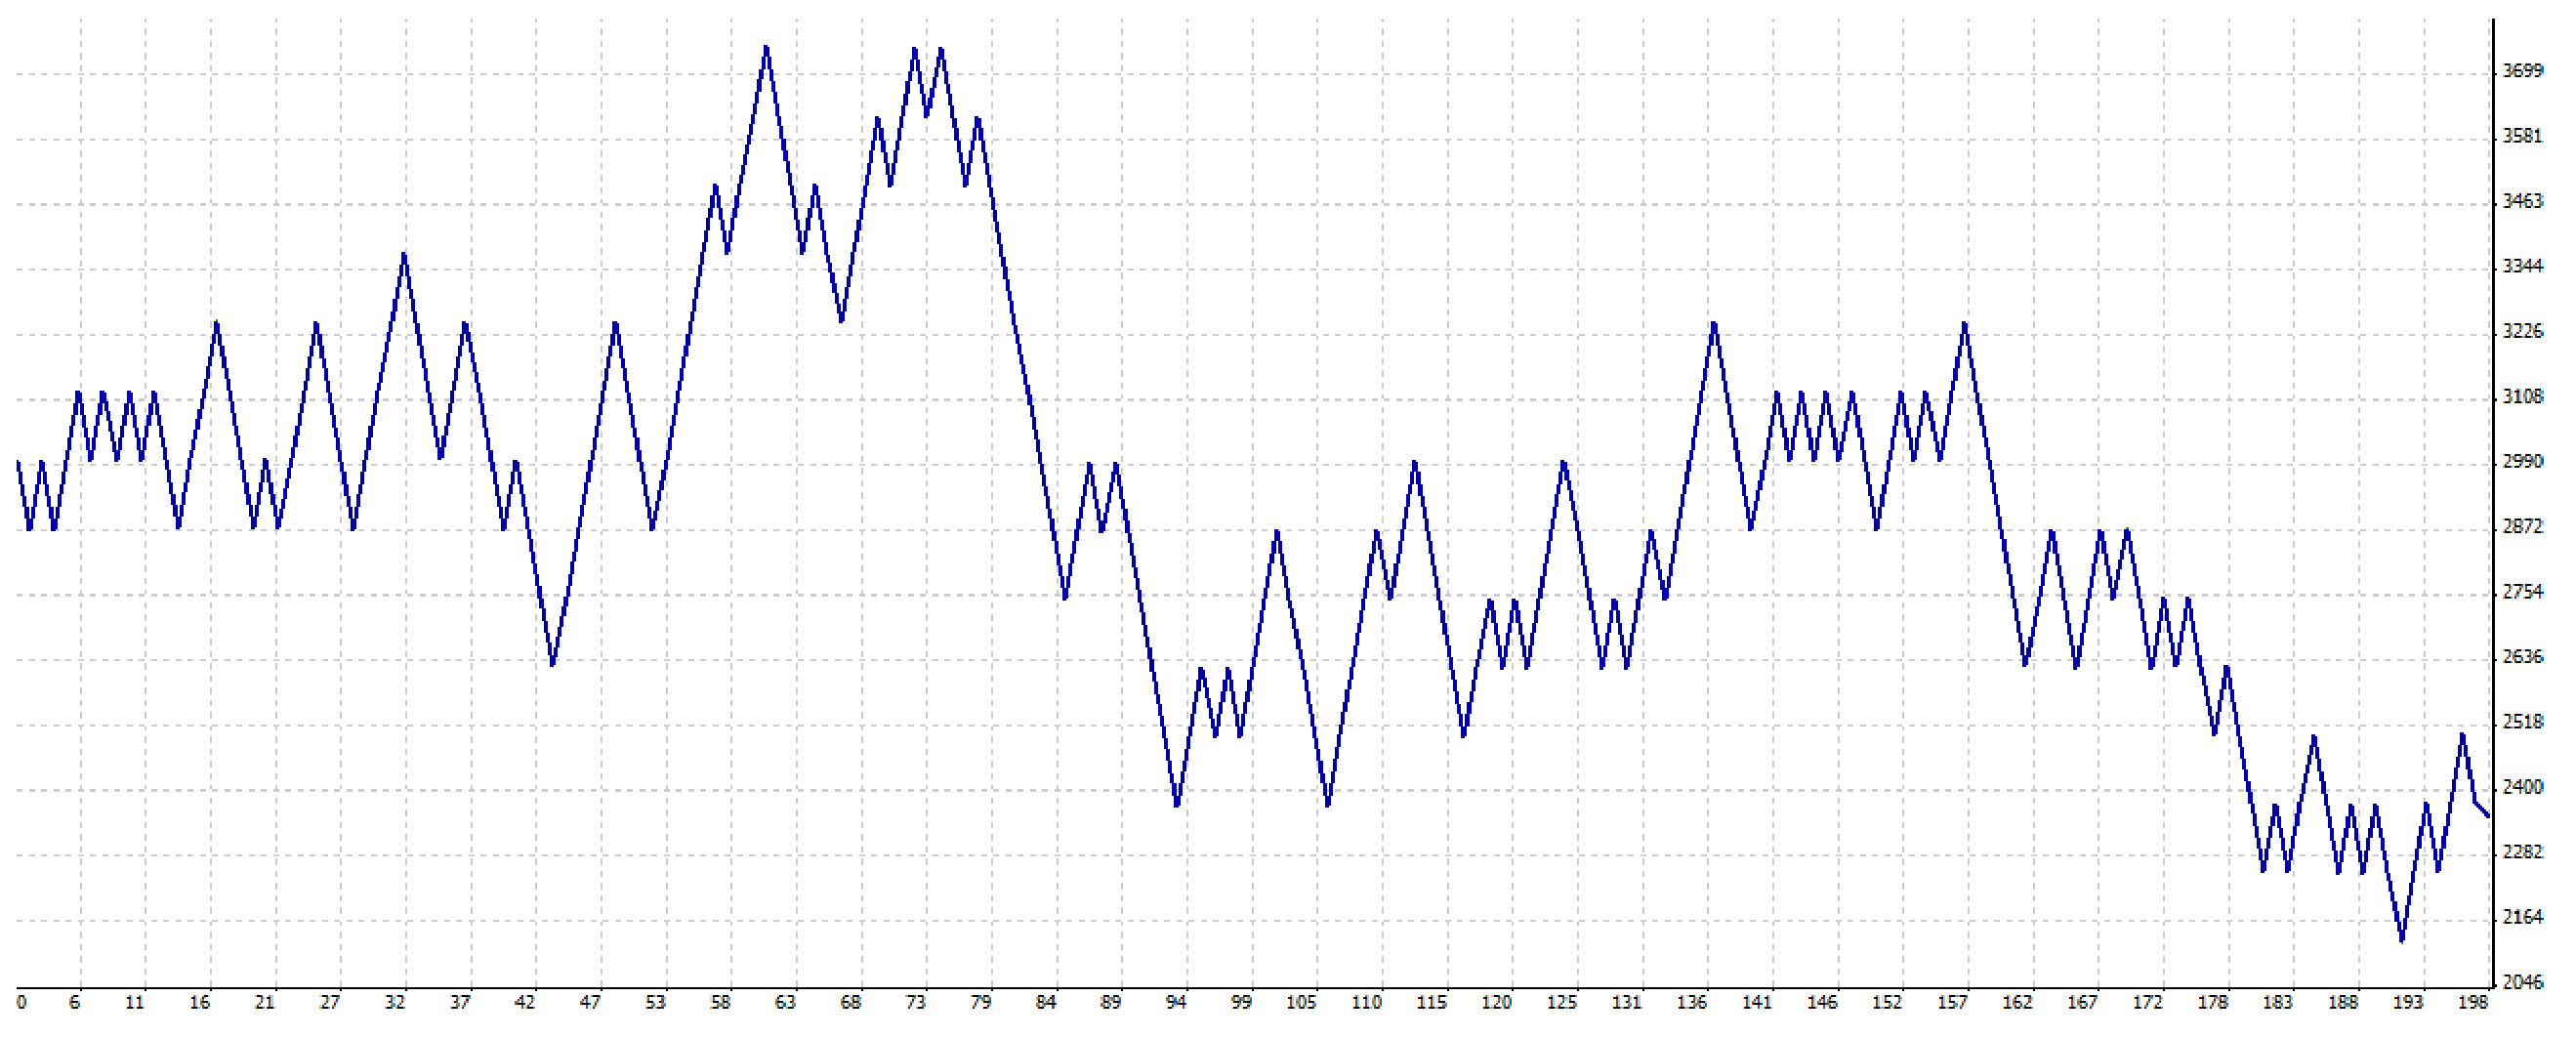
\includegraphics[width=0.9\textwidth]{figuras/protocoloMedia4}
\caption{ Gráfico gerado pela simulação do \textit{expert} MediaMovel.mql no período de Agosto de 2013 a Agosto de 2014} 
\label{protocoloMedia4}
\end{figure}


\subsection{Definição dos métodos de operação software InvestMVC}

Os Métodos Matemáticos de Correlação Linear, Fibonacci e Mínimos Quadrados tiveram êxito nos dois anos de simulação (Agosto 2012 a Agosto de 2014) e obtiveram lucro superior a 10\%  sob o capital inicial. Os métodos de Estocástico e Média Móvel tiveram prejuízo nos dois anos de simulação. Portanto, foram escolhidos os métodos de Correlação Linear, Fibonacci e Mínimos Quadrados como métodos de estratégia financeira do software InvestMVC.

A Tabela \ref{resultadoMetodos} evidencia os resultados financeiros de cada Método Matemático em percentual de negociações com lucro. Isso reforça o motivo da escolha dos métodos Correlação Linear, Fibonacci e Mínimos Quadrados.


\begin{center}
\begin{longtable}{ | p{6cm} | p{3cm}| p{3cm} |}
\caption{Percentual de negociações com lucro dos Métodos Matemáticos} \\
\hline
\textbf{Método Matemático} & \textbf{Percentual de lucro em 2012 – 2013} & \textbf{ Percentual de lucro em 2013 – 2014}\\ \hline
\endfirsthead
\multicolumn{3}{c}%
{\tablename\ \thetable\ -- \textit{Continuação da página anterior}} \\
\hline
\textbf{Método Matemático} & \textbf{Percentual de lucro em 2012 – 2013} & \textbf{Percentual de lucro em 2013 – 2014}\\
\endhead
\hline \multicolumn{3}{c}{\textit{Continuação na próxima página}} \\
\endfoot
\hline
\endlastfoot
Mínimos Quadrados& 77.88\%  & 85.71\%  \\
Fibonacci& 72.73\%& 56.00\% \\
Correlação Linear& 56.86\%& 55.56\%  \\
Média Móvel& 43.48\%& 48.48\%\\
Estocástico& 47.47\% & 47.70\%
\label{resultadoMetodos}
\end{longtable}
\end{center}

\section{Estruturas e Componentes do software InvestMVC}
Esta seção evidencia as estruturas e componentes do software InvestMVC. Este resultado atende o Objetivo Específico 2 (caracterizar as estruturas e componentes) deste trabalho.
Uma arquitetura Orientada a Componentes possui o propósito de dividir para conquistar. Um grande problema é subdividido em partes menores e em seguida se desenvolve soluções mais elaboradas \cite{john}.

Por usar vários paradigmas, o software InvestMVC tem vários componentes, sendo cada qual implementado em um paradigma de programação mais adequado às necessidades do componente bem como contendo responsabilidades bem definidas. A Figura \ref{componente} procura ilustrar esses componentes usando a representação de digrama de classes.

\newpage
\begin{figure}[H]
\centering
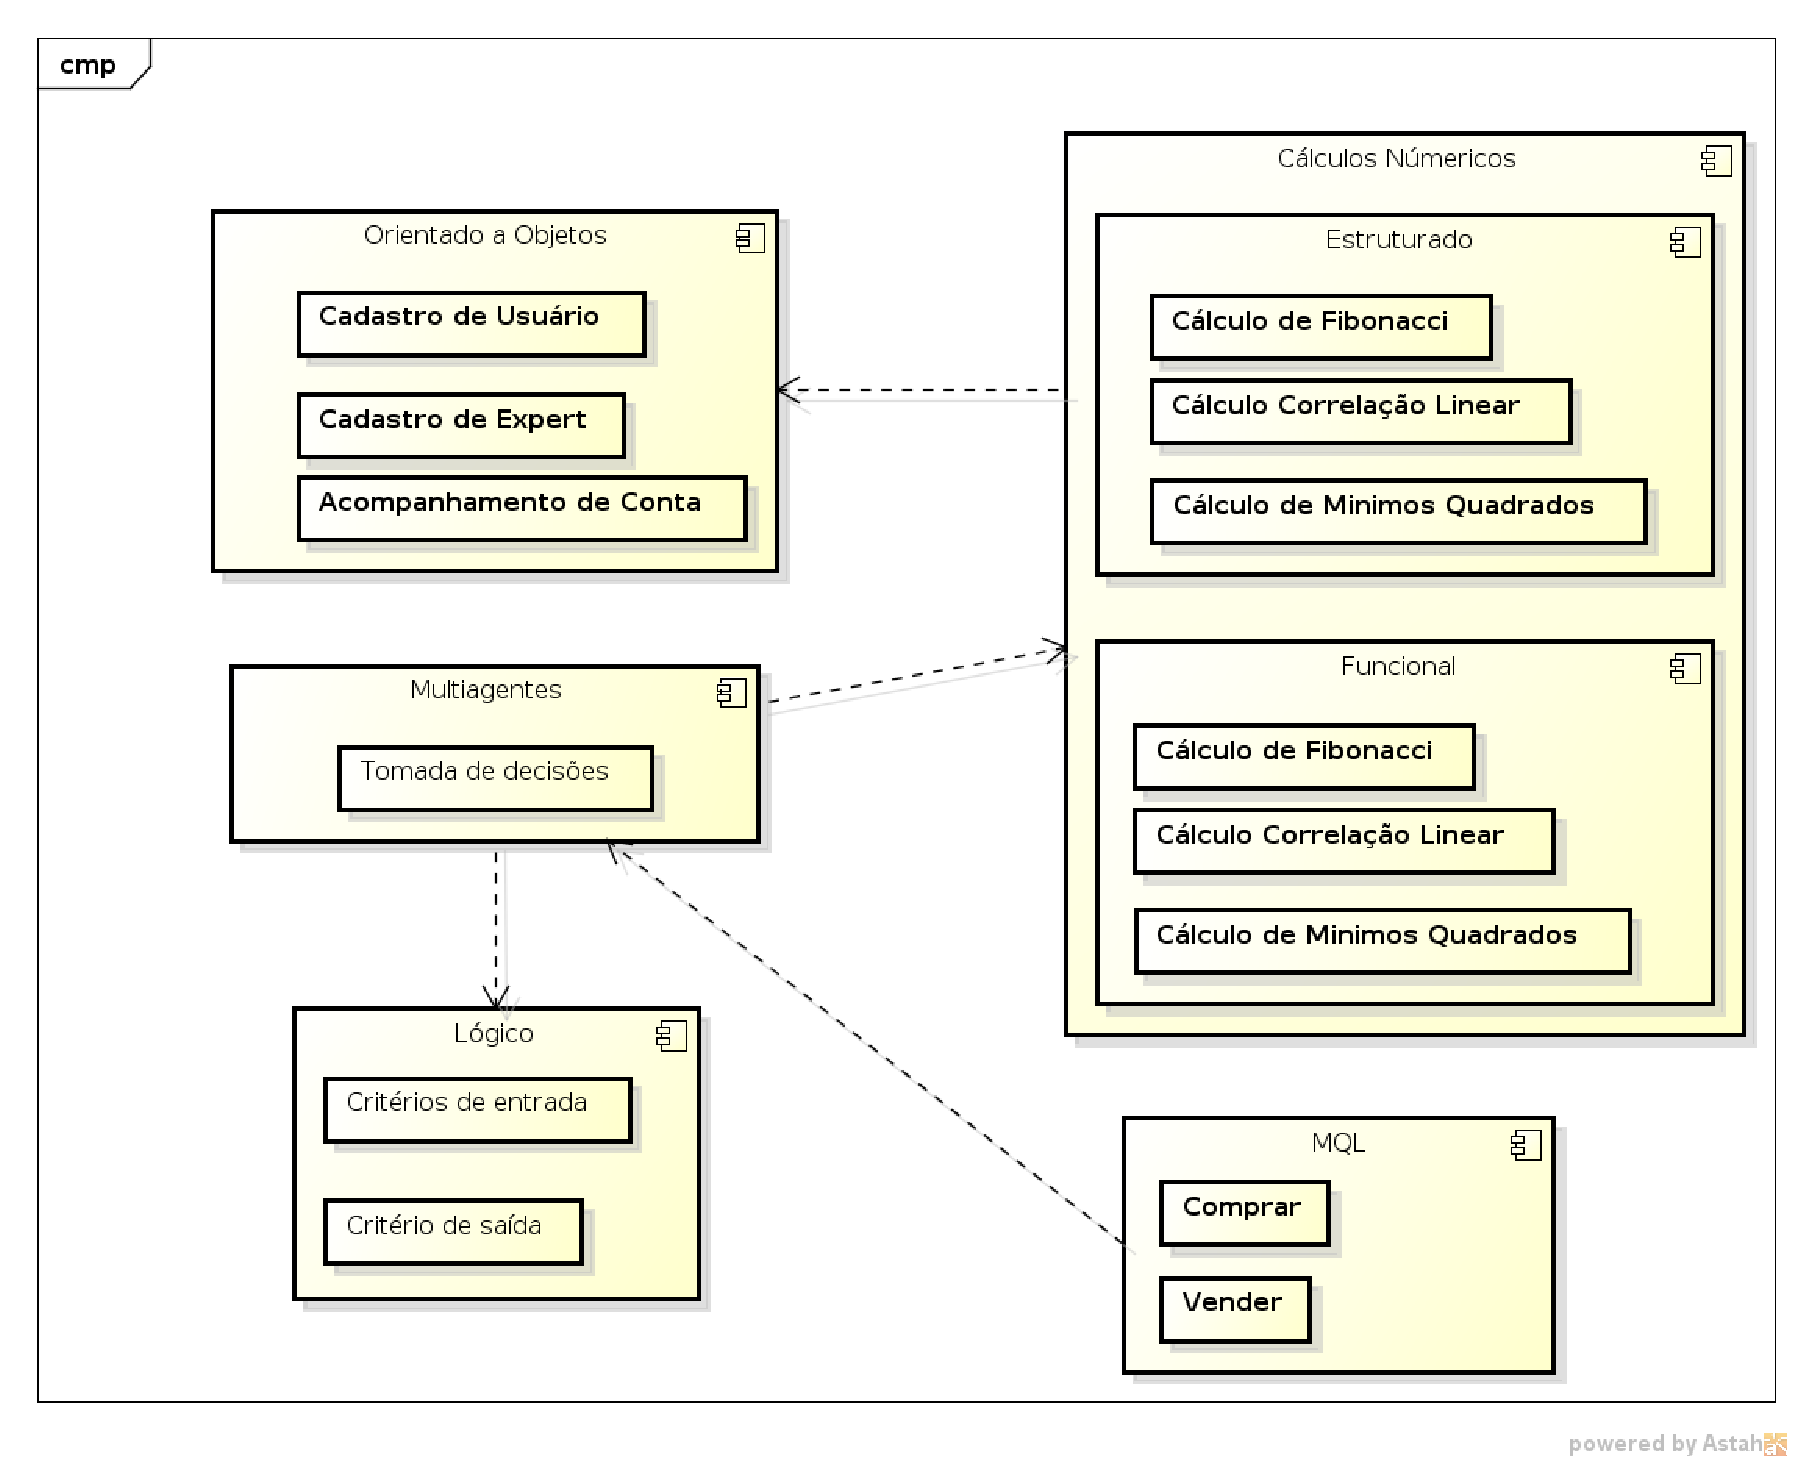
\includegraphics[width=0.9\textwidth]{figuras/componente}
\caption{Diagrama de Classe InvestMVC}
\label{componente}
\end{figure}

\subsection{Componente Orientado a Objetos}

Este componente é o responsável pela interação com o usuário e foi implementado em linguagem Groovy. A escolha dessa linguagem, se deu porque esta é voltada para aplicações web e juntamente com  o framework grails, fornece a criação de um projeto com uma arquitetura MVC definida, como demonstra a Figura \ref{classeOO}.

\newpage
\begin{figure}[H]
\centering
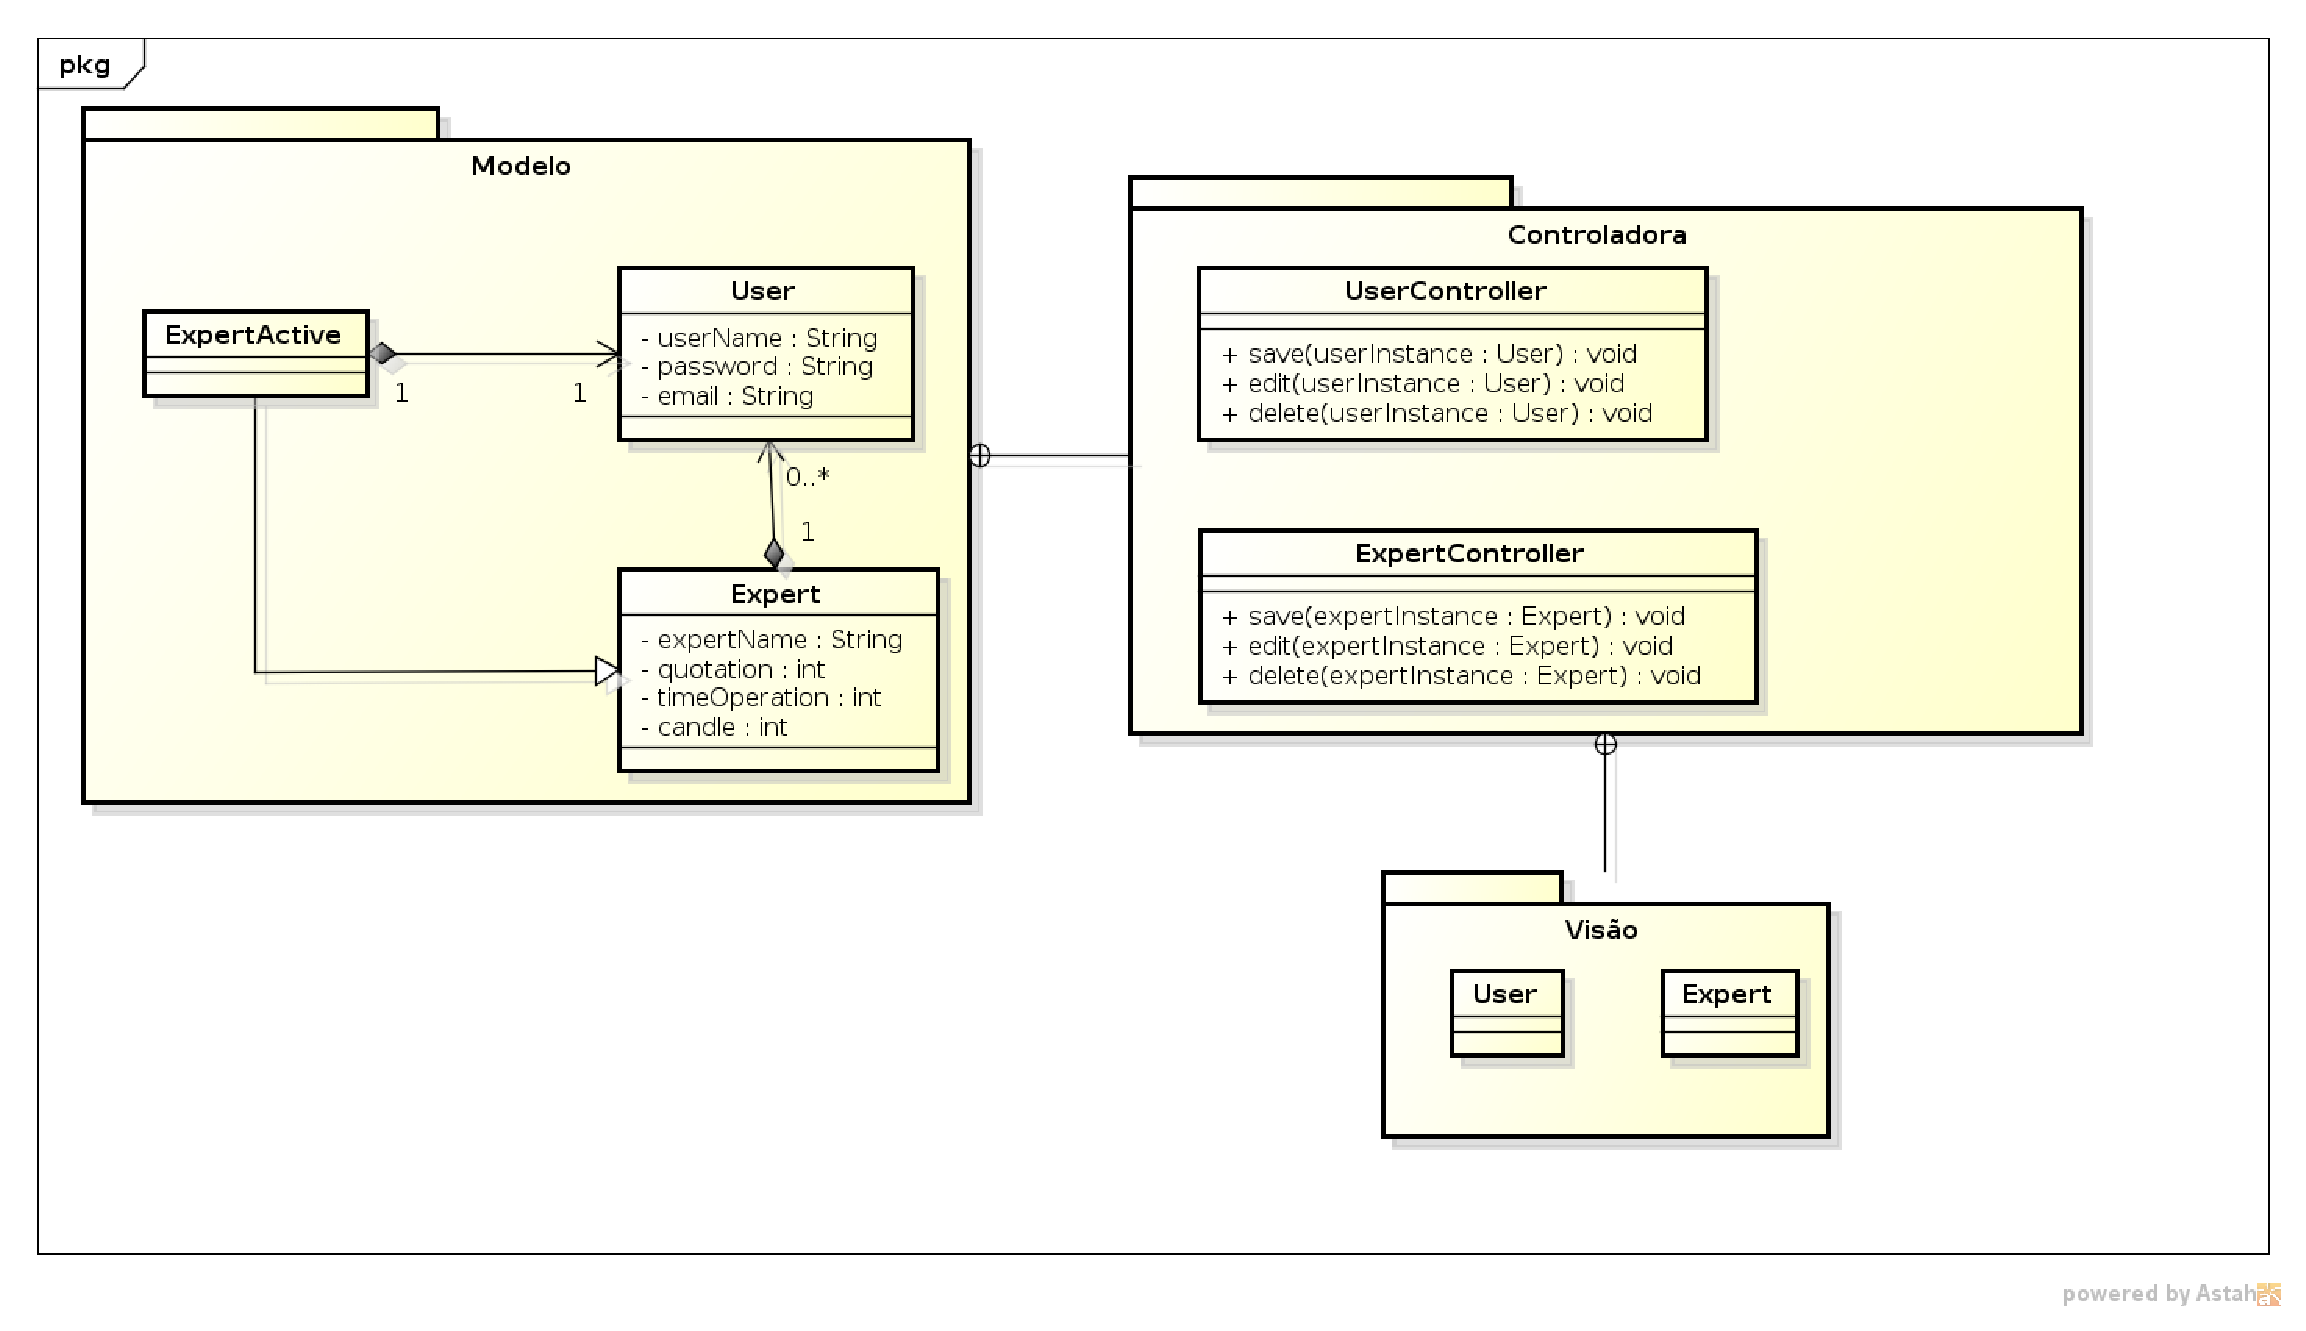
\includegraphics[width=0.9\textwidth]{figuras/classeOO}
\caption{Diagrama de Classe InvestMVC componente Orientado a Objetos} 
\label{classeOO}
\end{figure}

Segundo \citeonline{lamin} na arquitetura MVC, o controle de fluxo de dados ocorre de forma específica. Orientando-se por esse autor, o fluxo de dados dentro do componente Orientado a Objetos do software InvestMVC ocorre da seguinte forma:

\begin{enumerate}
\item O usuário, neste caso o investidor, interage com a Visão.
\item A Controladora manipula o evento da interface do usuário por meio de uma rotina.
\item A Controladora acessa a camada de Modelo, atualizando-a com base nas interações do usuário.
\end{enumerate}

O diagrama de sequência do componente Orientado a Objetos é evidenciado na Figura \ref{sequenciaOO}.

\newpage
\begin{figure}[H]
\centering
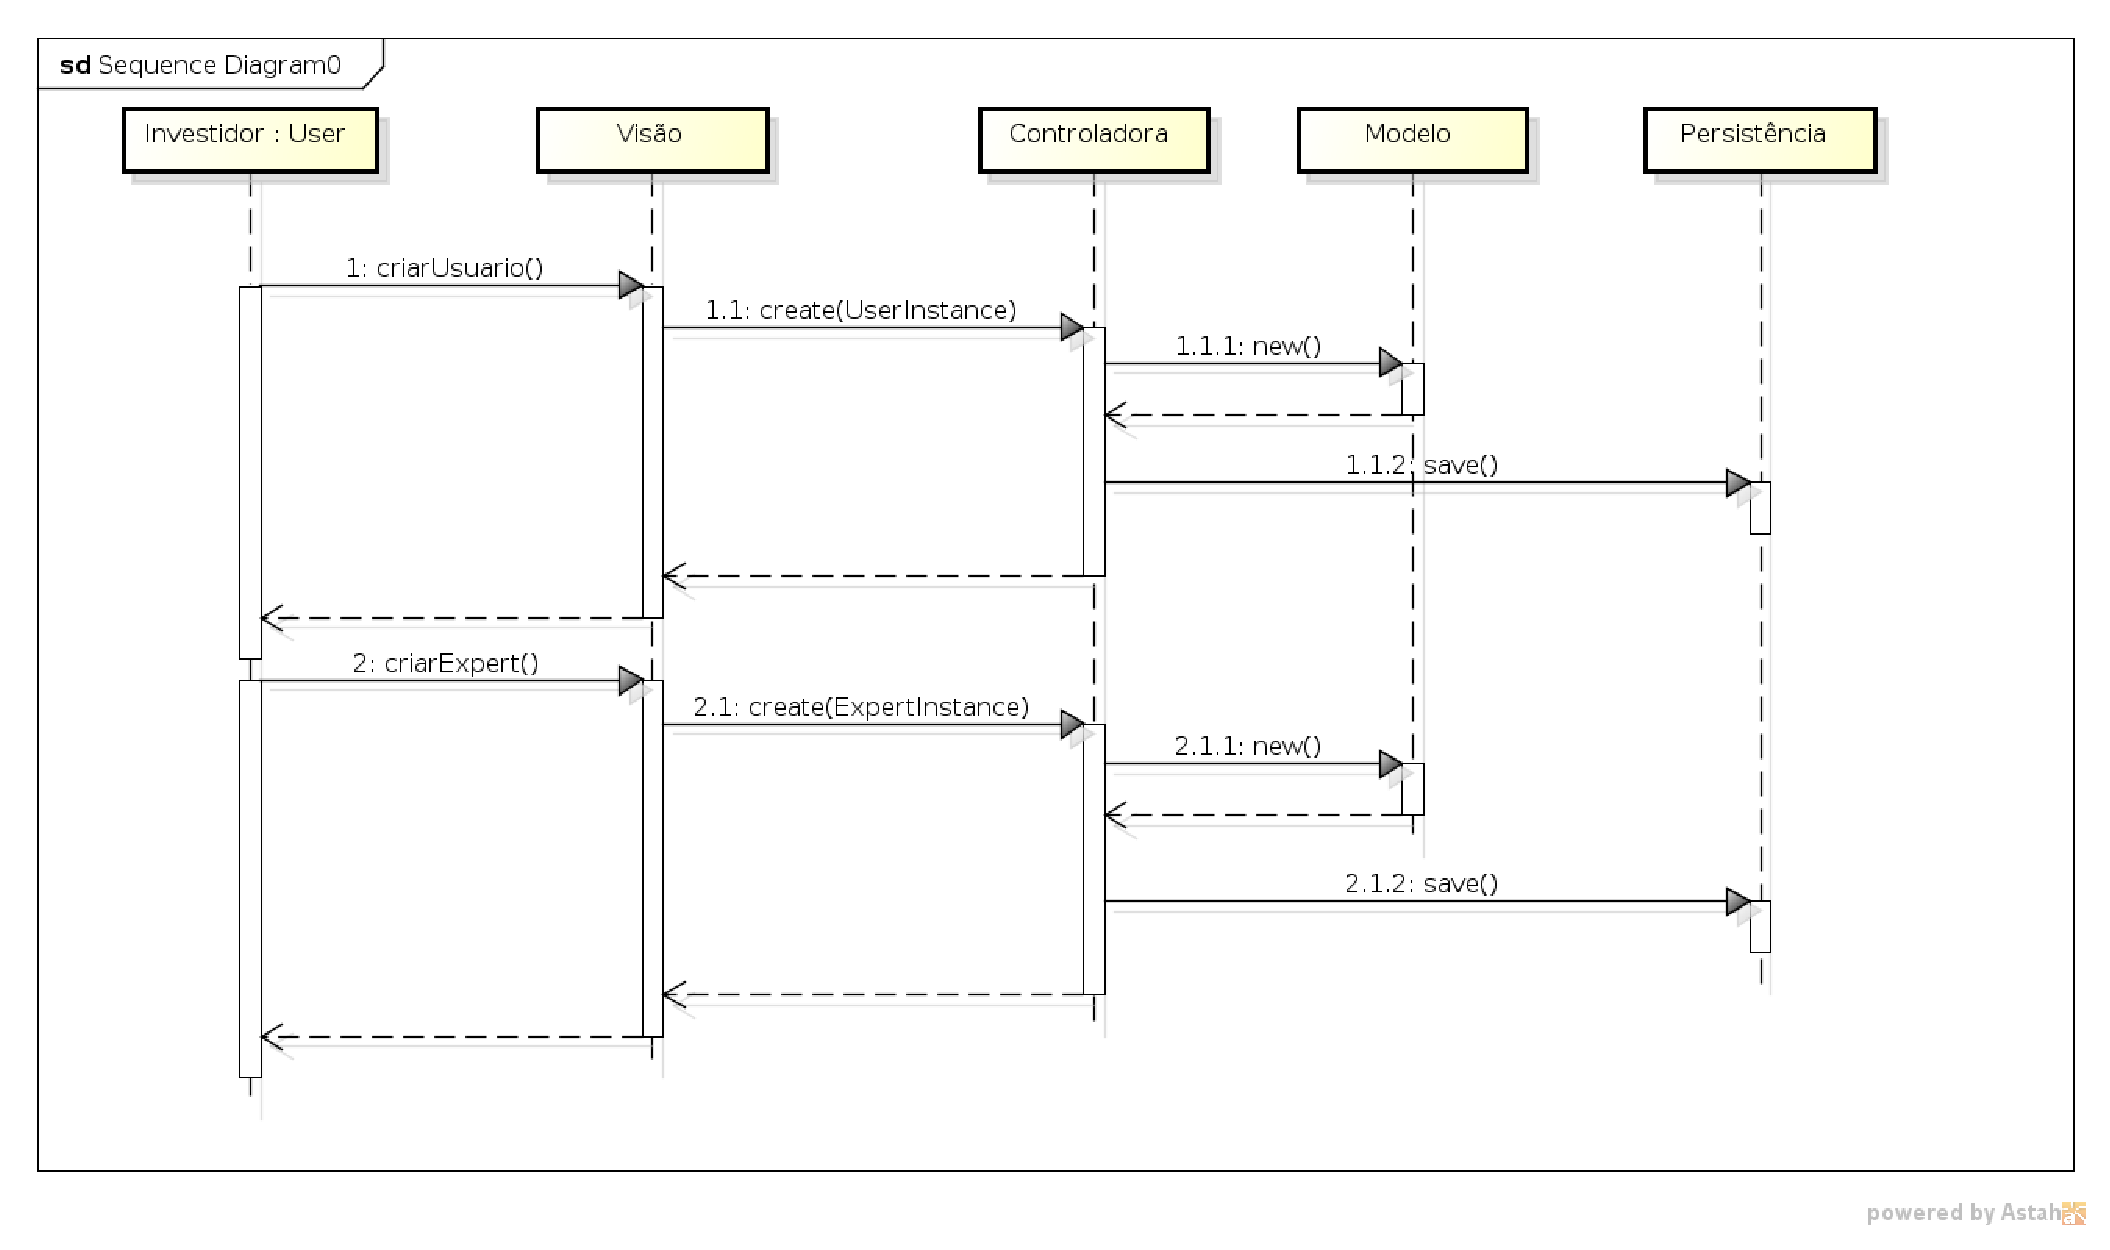
\includegraphics[width=0.9\textwidth]{figuras/sequenciaOO}
\caption{Diagrama de sequência InvestMVC componente Orientado a Objetos}
\label{sequenciaOO}
\end{figure}

As classes mais relevantes do componente Orientado a Objetos encontram-se no Apêndice \ref{ap:oo}.

\subsection{Componente Cálculos Numéricos}

O componente Cálculos Numéricos é responsável por calcular os Métodos Matemáticos presentes no software InvestMVC. Este módulo é composto por dois outros componentes: componente Estruturado e componente Funcional.

O componente Estruturado do software InvestMVC foi programado em linguagem C e o módulo Funcional em linguagem Haskell. Ambos os componentes realizam os mesmos cálculos. Isso aumenta a probabilidade de não ocorrer erros nos cálculos dos Métodos Matemáticos. Caso um dos componentes, por algum motivo, não seja executado no momento correto, a tendência é que o outro módulo realize os cálculos.

\subsection{Componente Funcional}
Na linguagem Haskell, por ser uma linguagem de programação funcional, sua "gramática" está próxima das funções matemáticas, logo a implementação dos métodos algébricos e numéricos se torna muito intuitiva \cite{hoogle2013}.

O paradigma funcional é declarativo. Por limitar o uso de atribuições às variáveis, evitando a noção de estados (comum no paradigma  estruturado bem como na Orientação a Objetos), os resultados das funções em Haskell são mais precisos do que em outros paradigmas \cite{piponi2006}.

Devido estes fatos , o paradigma funcional foi utilizado para implementar os Métodos Matemáticos de Correlação Linear, Mínimos Quadrados e Fibonacci. Por ser simples, este componente será formado apenas por quatro arquivos em Haskell, cada arquivo realiza o cálculo de um método matemático.

\begin{figure}[H]
\centering
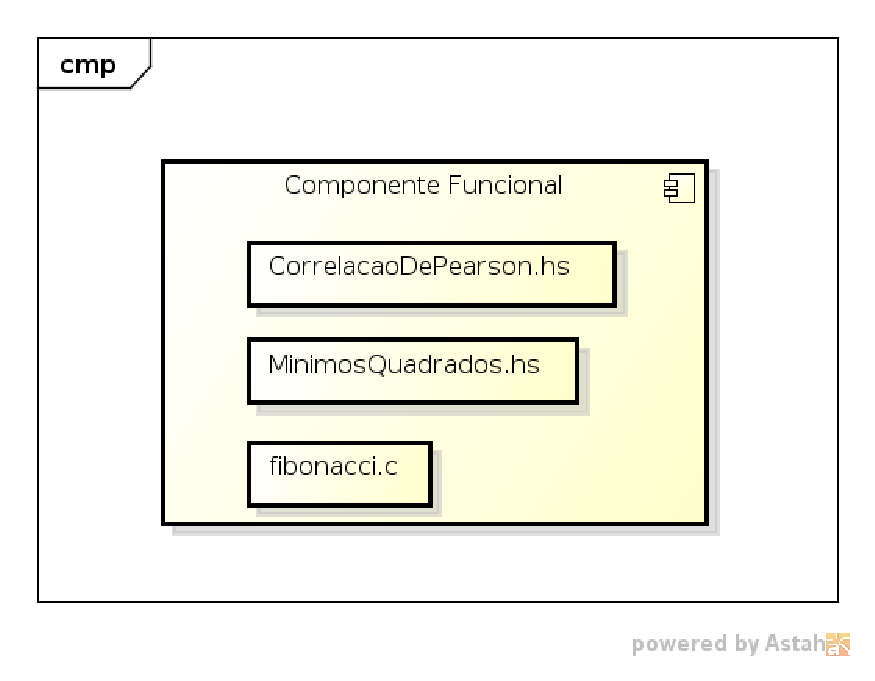
\includegraphics[width=0.5\textwidth]{figuras/componenteFuncional}
\caption{Componente Funcional InvestMVC} 
\label{componenteFuncional}
\end{figure}

O componente Funcional espera uma socilitação de cálculo do componente Multiagente. Logo após a solicitação, o componente busca na camada de persistência (representado por um sistema de arquivos) as cotações do mercado. Com essas cotações o componente é capaz de realizar o cálculo do método matemático, o qual é esperado pelo componente Multiagente, como é mostrado na Figura \ref{sequenciaFuncional}.

\begin{figure}[H]
\centering
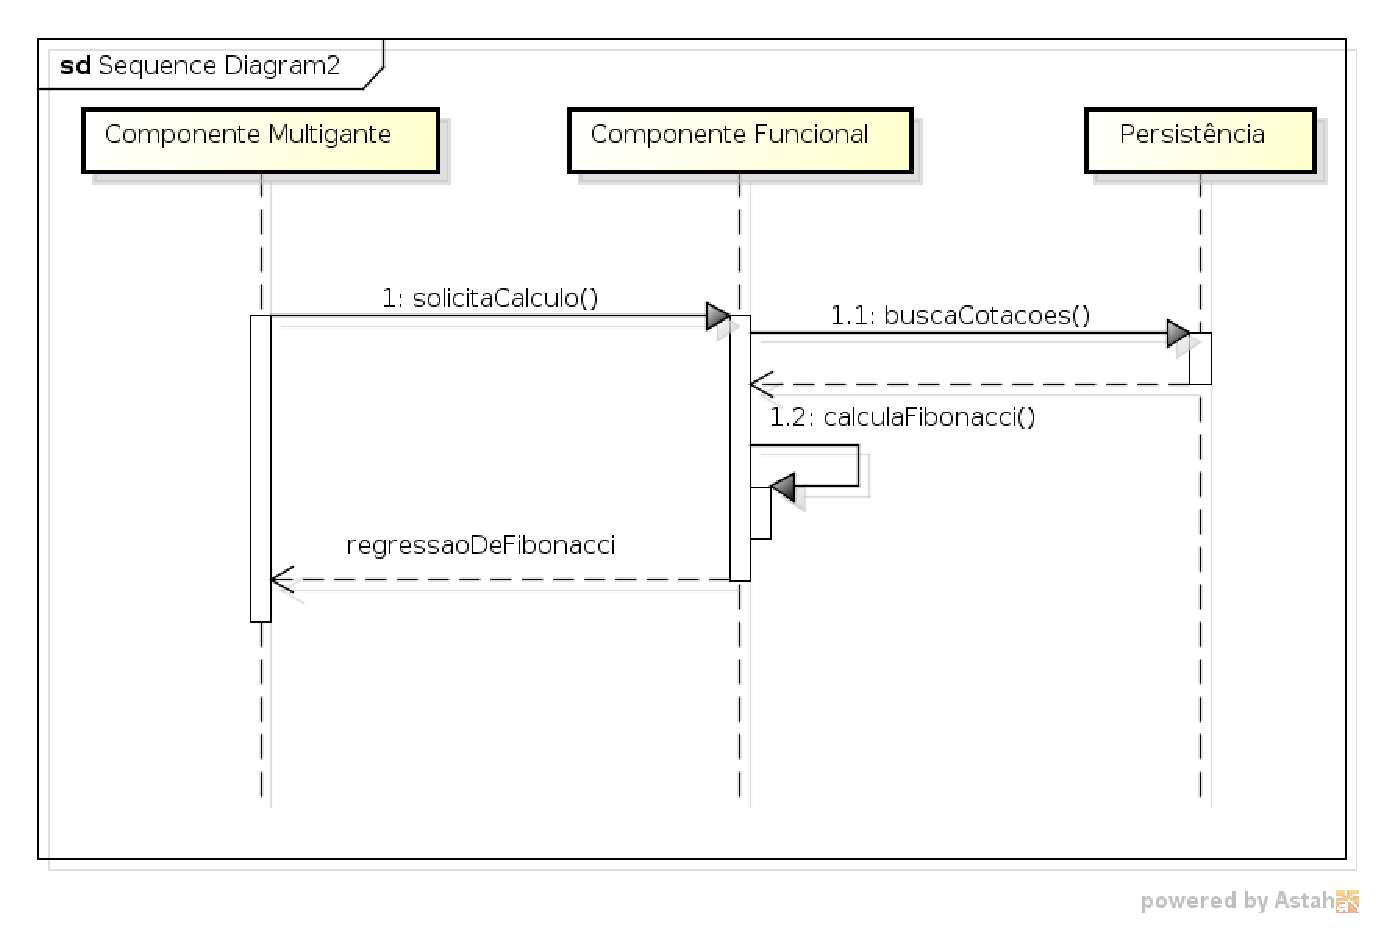
\includegraphics[width=0.9\textwidth]{figuras/sequenciaFuncional}
\caption{Diagrama de Sequência do Componente Funcional InvestMVC} 
\label{sequenciaFuncional}
\end{figure}

\subsection{Componente Estruturado}

A linguagem de programação C é estruturada, possuindo a vantagem da velocidade de execução do código-fonte. Também é uma linguagem bastante utilizada para realizar cálculos numéricos e algébricos \cite{gustavo}. 

O paradigma estruturado utilizando a linguagem C também foi utilizado para implementar os Métodos Matemáticos de Correlação Linear, Mínimos Quadrados e Fibonacci.

A arquitetura bem como a sequência do fluxo de dados do Componente Estruturado seguem a mesma lógica do Componente Funcional, como ilustrado na Figura \ref{sequenciaEstruturado}.

\begin{figure}[H]
\centering
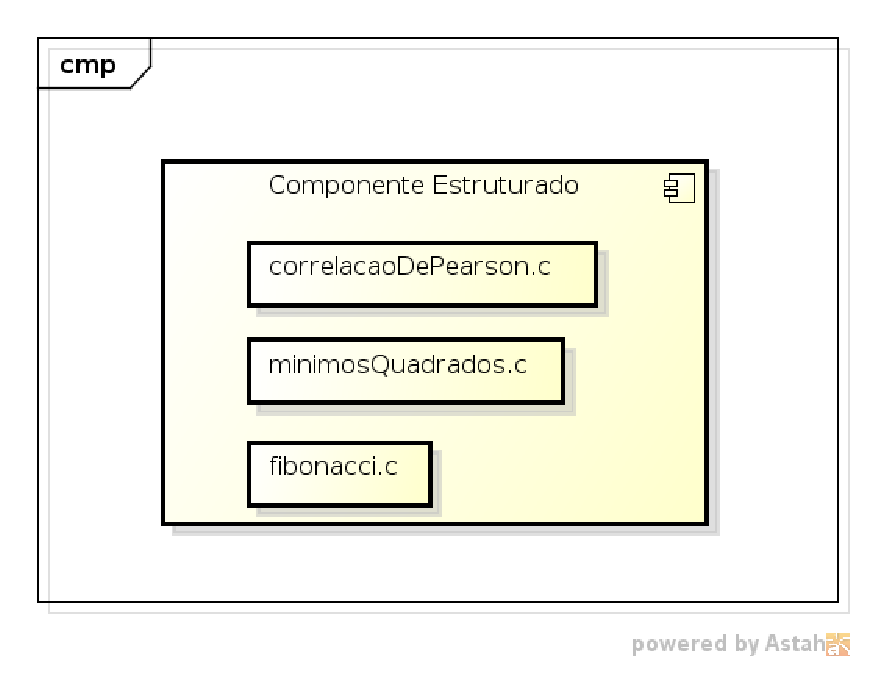
\includegraphics[width=0.7\textwidth]{figuras/componenteEstruturado}
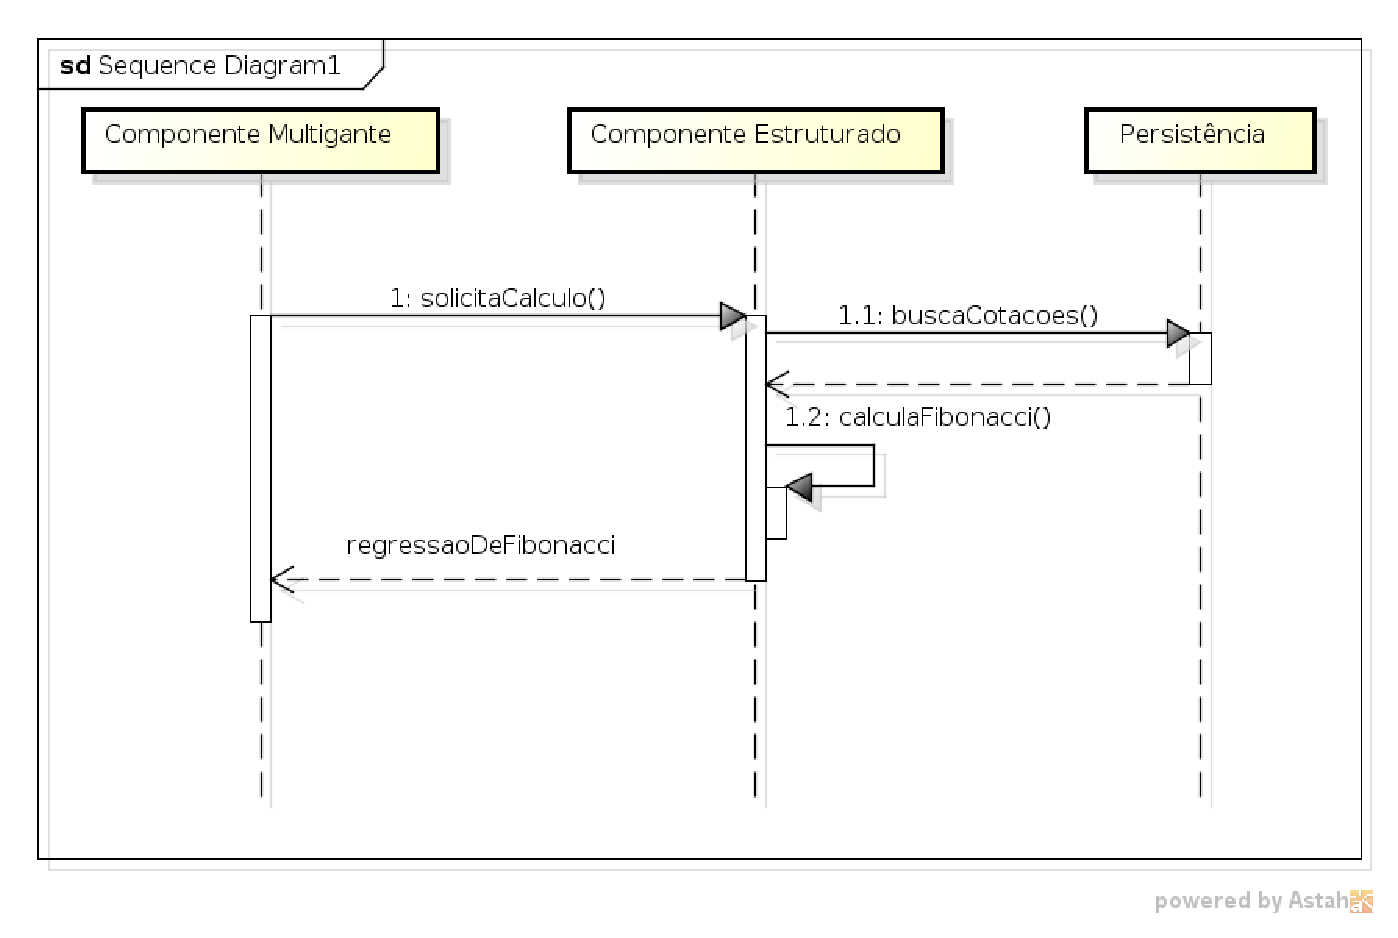
\includegraphics[width=0.7\textwidth]{figuras/sequenciaEstruturado}
\caption{Diagramas de Componentes e de Sequência do Componente Estruturado InvestMVC.}
\label{sequenciaEstruturado}
\end{figure}

\subsection{Componente Multiagente}

O componente Multiagente foi implementado usando o paradigma Multiagente com a linguagem Java e o apoio da Plataforma JADE.

\begin{citacao}
O JADE se trata de um \textit{framework} de software, independente de aplicação específica, capaz de prover funcionalidades de camada \textit{middleware}. Ele possui uma infraestrutura bastante flexível para o desenvolvimento de aplicações onde o elemento de abstração é um agente de  software. Para isso ele oferece suporte ao ciclo de vida e a lógica do núcleo de agentes em si, além de oferecer uma variedade de ferramentas gráficas que favorecem o desenvolvimento. A tecnologia é totalmente escrita em Java, o que traz benefícios a partir do enorme conjunto de recursos e bibliotecas oferecidas pela linguagem, que por sua vez oferece um vasto conjunto de abstrações de programação e possibilita a construção de sistemas baseados em agentes com competências relativamente mínimas em relação à teoria de agentes. Com isso, o programador pode economizar o tempo com o trabalho inicial necessário para construir uma infraestrutura baseada em agentes, e dedicar seus esforços para o negócio da aplicação propriamente dito \cite{teixeira2010}. 
\end{citacao}

Agentes de software são entidades autônomas e com capacidades sociais. O uso deste paradigma foi justificado dada as colocações realizadas na etapa de tomada de decisões desse trabalho \cite{agentBuilderWhy}. 

Os agentes do software  InvestMVC possuem uma arquitetura reativa, pois suas ações se dão pelas variações que ocorrem nas cotações do Mercado de Moedas.

A arquitetura do Componente Multiagente está modularizada por pacotes: o pacote comportamentos é formado por compormentos que são usados pelos Agentes de Software; o pacote metodosMatemáticos é formado por Agentes que acessam o componente Cálculos matemáticos; o pacote investidores é composto por agentes que interagem com o Componente MQL, e o pacote execucao inicia a execução do SMA.

\newpage
\begin{figure}[H]
\centering
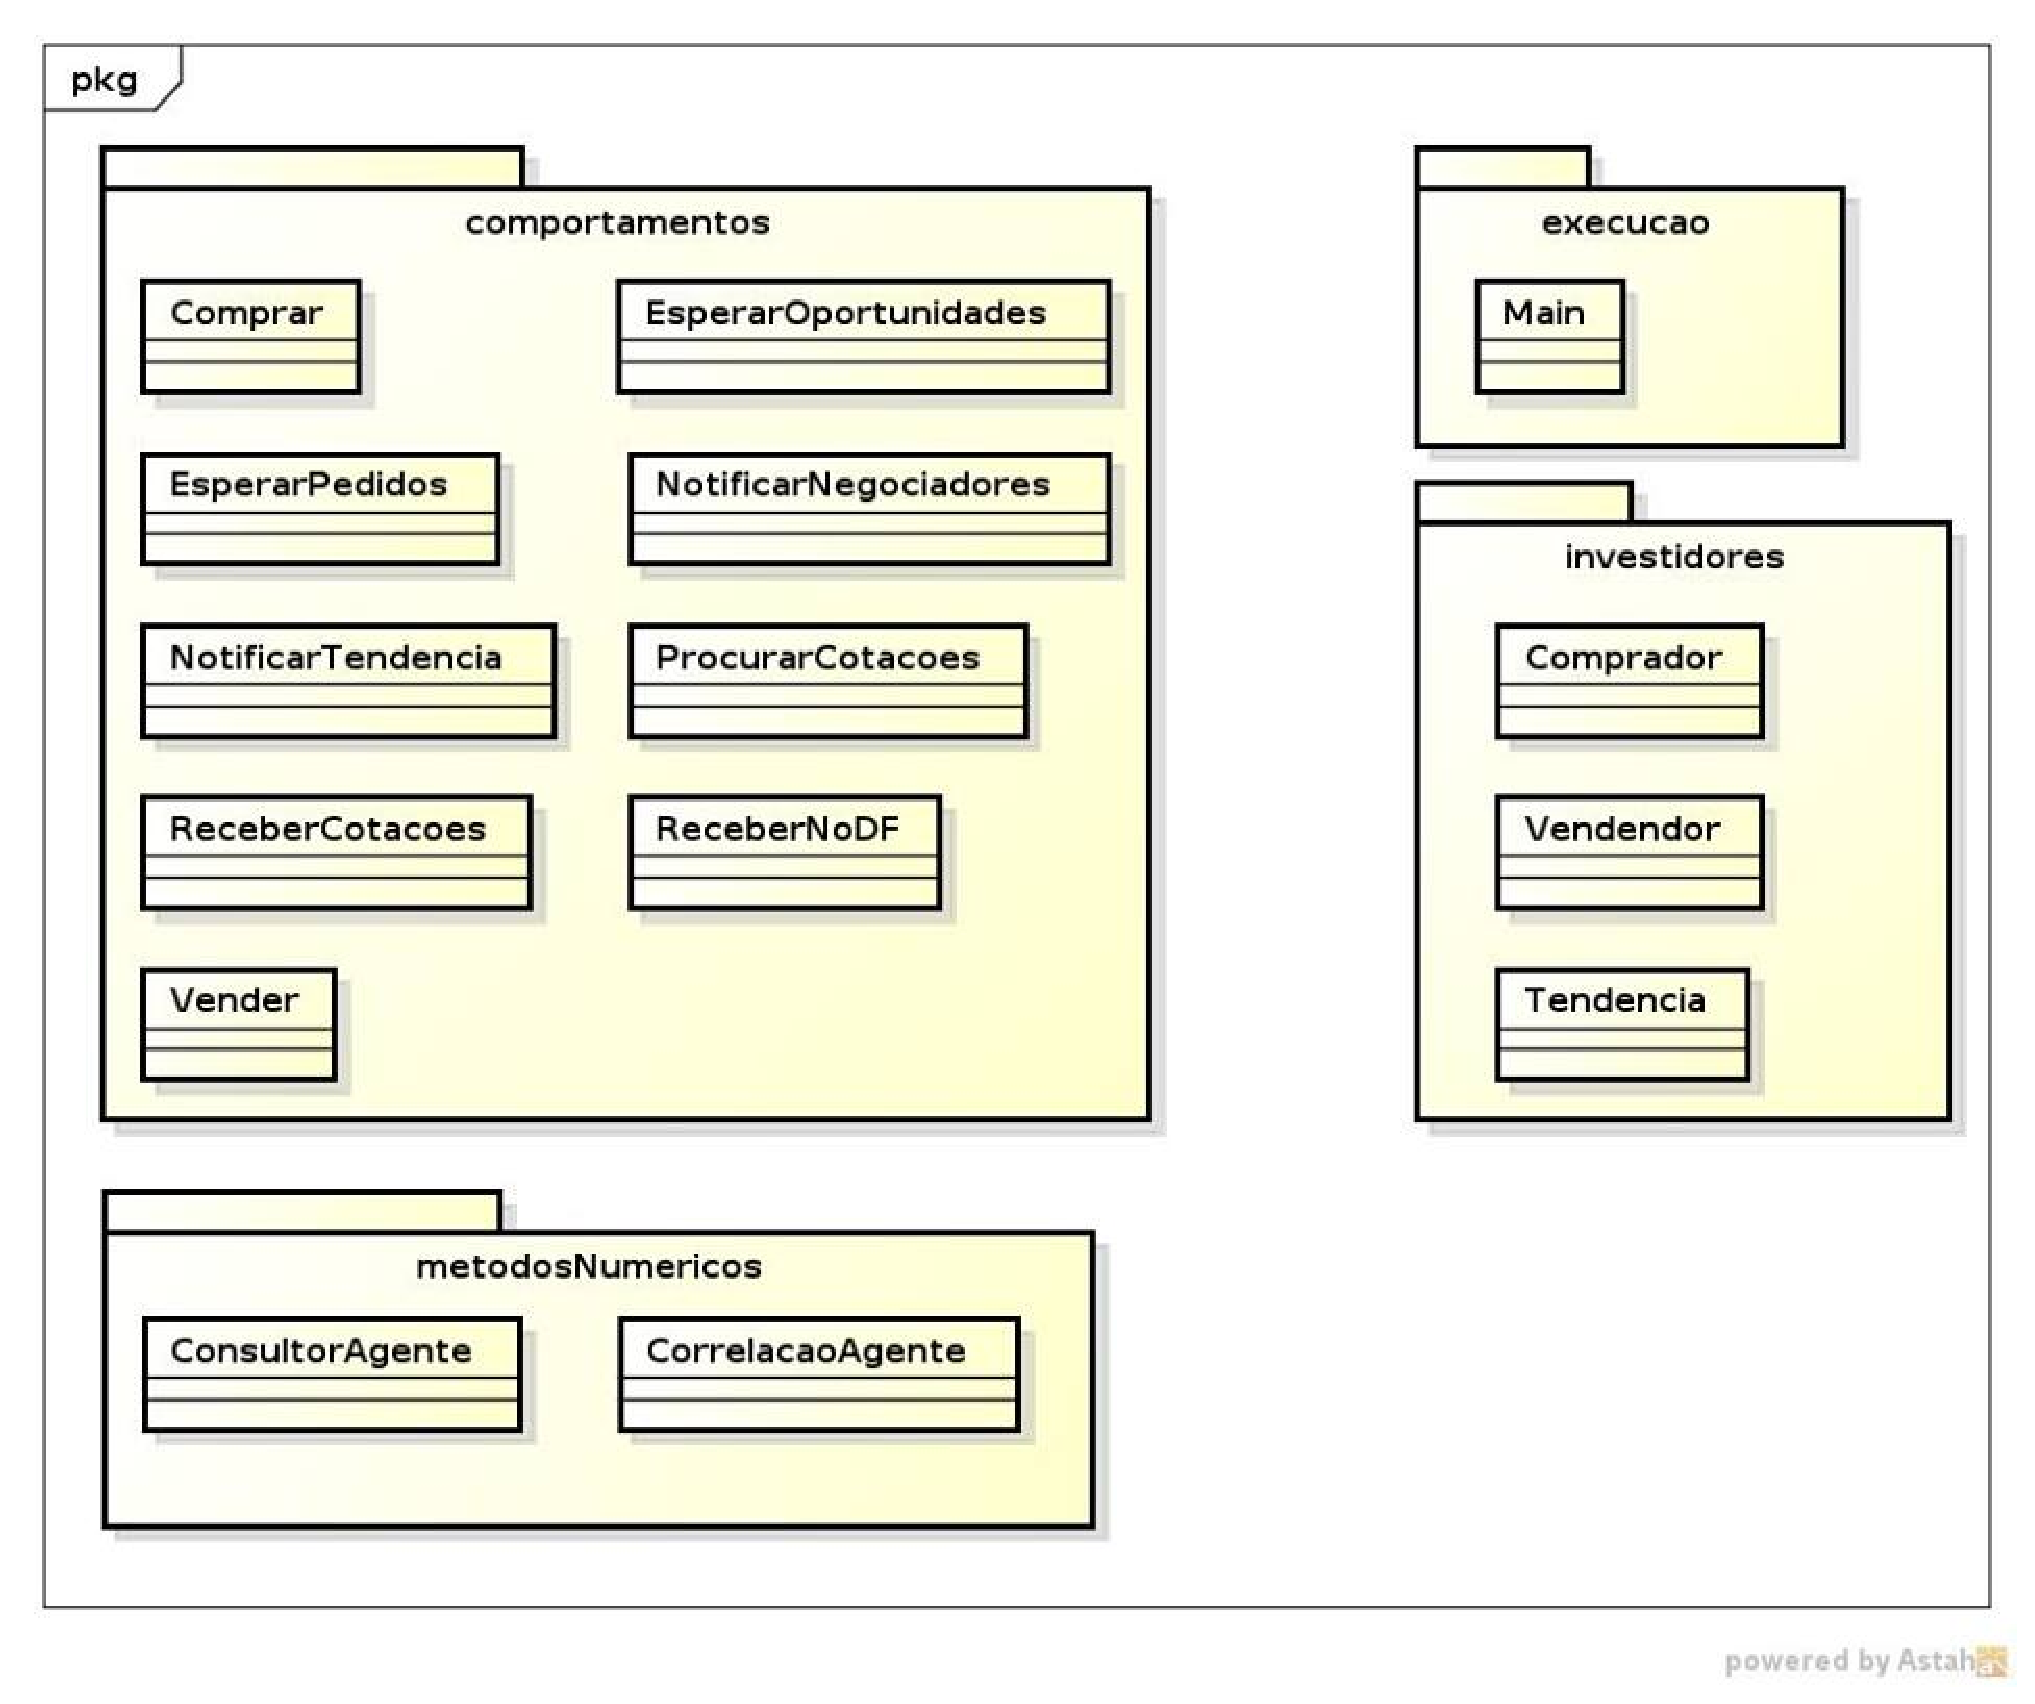
\includegraphics[width=0.9\textwidth]{figuras/diagramaClassesSMA}
\caption{Diagrama de Classe do Componente Multiagente InvestMVC} 
\label{diagramaClassesSMA}
\end{figure}

\subsection{Componente Lógico}

O componente Lógico foi produzido em linguagem Prolog, definindo uma base de conhecimento, a qual serve como critério de entrada e saída no Mercado de Moedas.

O paradigma Lógico facilita a representação, inserção e recuperação de conhecimento, por isso é muito usado em aplicações com Inteligência Artificial \cite{almeida2010}.

A interação do Componente Lógico com o Componente Multiagentes é evidenciada na Figura \ref{sequenciaLogico}.

\newpage
\begin{figure}[H]
\centering
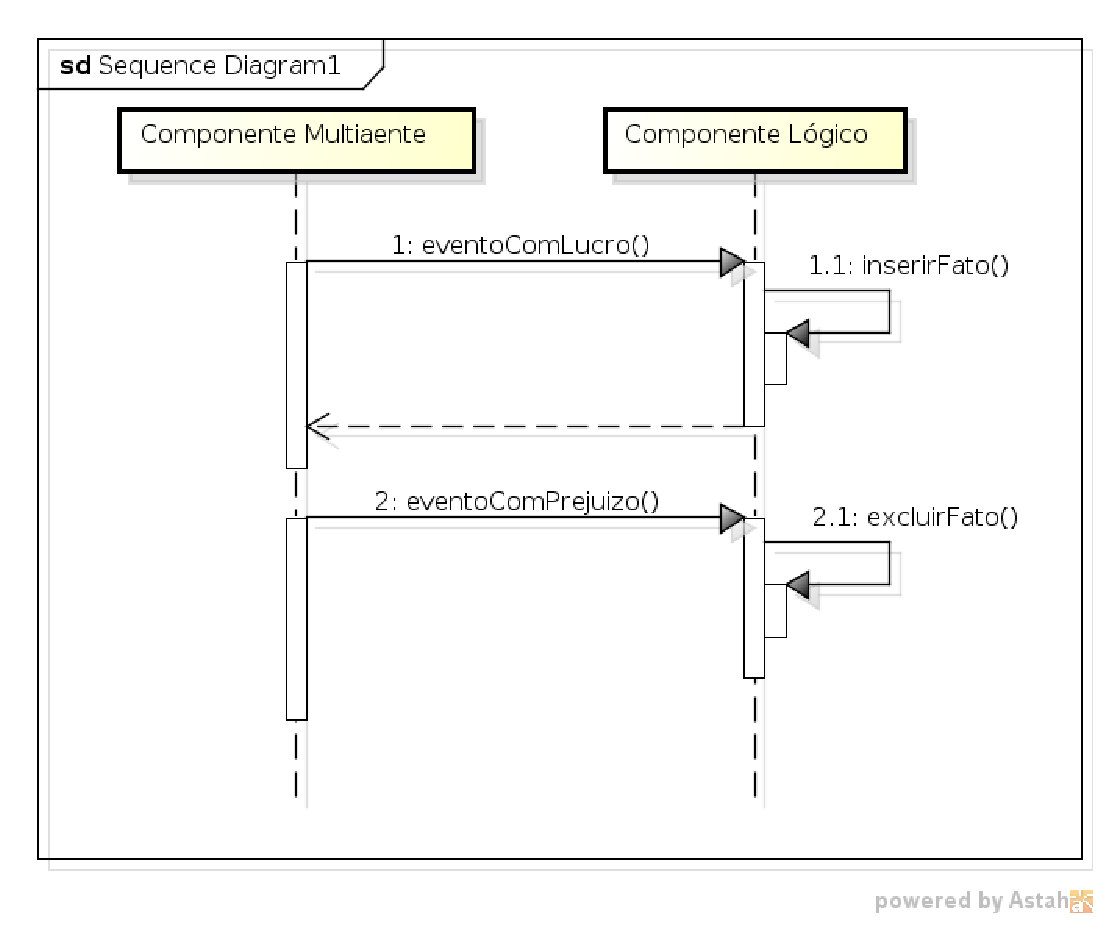
\includegraphics[width=0.7\textwidth]{figuras/sequenciaLogico}
\caption{Diagrama de Sequência do Componente Lógico InvestMVC.}
\label{sequenciaLogico}
\end{figure}

\subsection{Componente MQL}

O componente MQL é responsável por receber a resposta do Componente Multiagente para realizar uma compra ou venda. Adicionalmente, são recebidos outros atributos relacionados à compra ou venda, como alavancagem, \textit{stop loss} e \textit{take profit}, a implementação deste componente encontra-se no Apêndice \ref{ap:mql}.

A interação do Componente MQL com o Componente Multiagente é evidenciada na Figura \ref{sequenciaMQL}.

\begin{figure}[H]
\centering
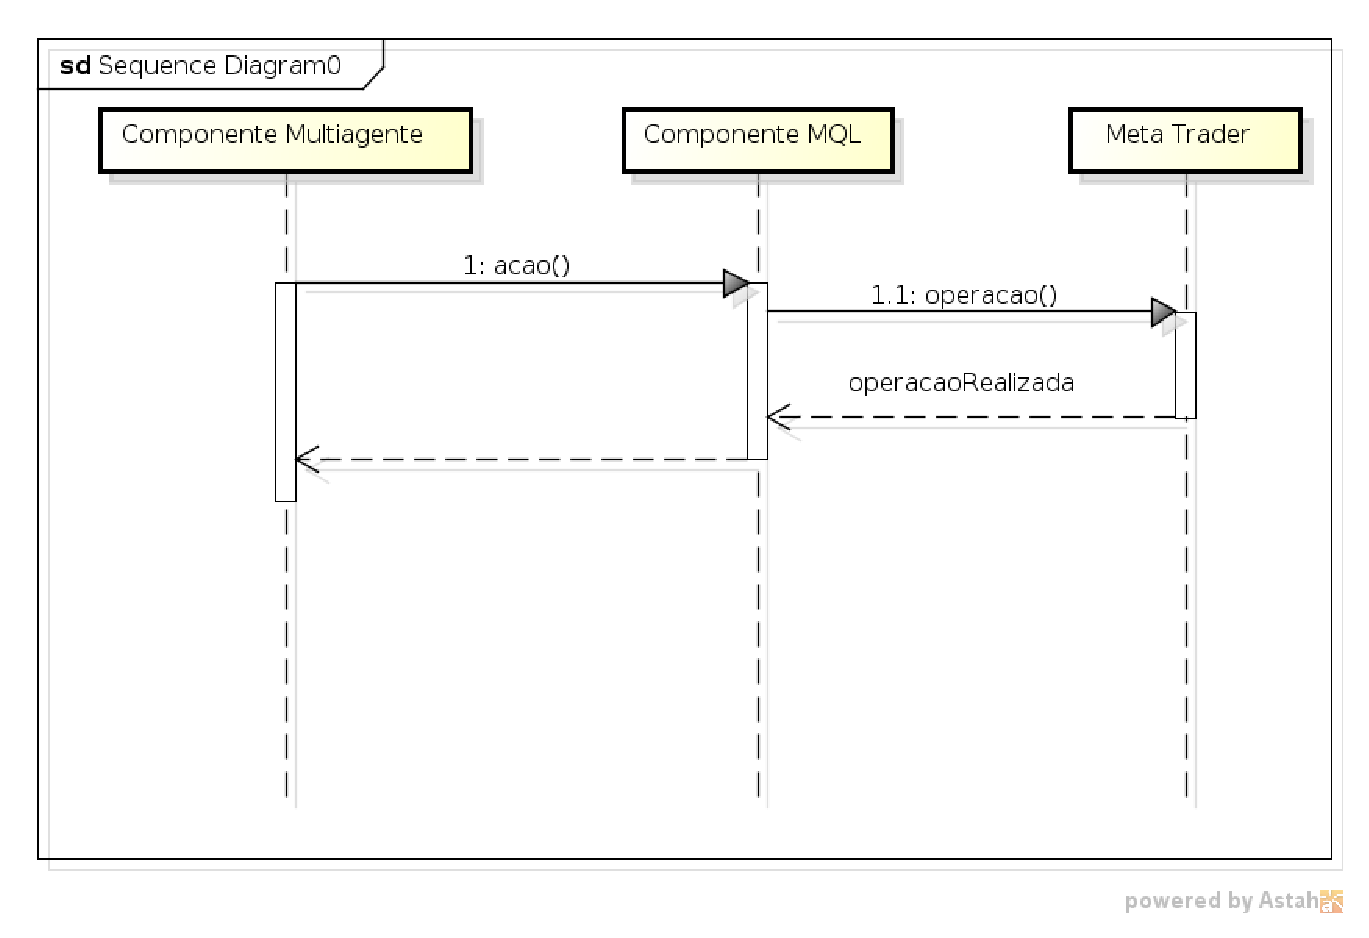
\includegraphics[width=0.5\textwidth]{figuras/sequenciaMQL}
\caption{Diagrama de Sequência do Componente MQL InvestMVC.}
\label{sequenciaMQL}
\end{figure}


\subsection{Fluxo de atividades}
O investidor interage apenas com o componente Orientado a Objetos, criando seu usuário e \textit{experts}, no qual serão persistidos. Além disso, o investidor também poderá ativar um \textit{expert}.

O componente Multiagentes vai verificar a tendência do Mercado de Moedas por meio da plataforma MetaTrader. Sendo assim, o componente Multiagentes buscará na persistência o \textit{expert} que está ativo. Sabendo qual o \textit{expert} que foi ativado, o componente Multiagente faz a requisição de cálculos para os módulos C e Haskell. A partir desse resultado, o componente Multiagente procurará no Módulo Base de Conhecimento, a alavancagem (quanto deve arriscar) e os valores de entrada para o método de Correlação de Pearson, Fibonacci e Mínimos Quadrados. Caso todas as especificações para o componente Multiagente sejam obedecidas, ele informa ao componente MQL para realizar uma compra ou venda. Esta interação é evidenciada na Figura \ref{sequencia}.

\begin{figure}[H]
\centering
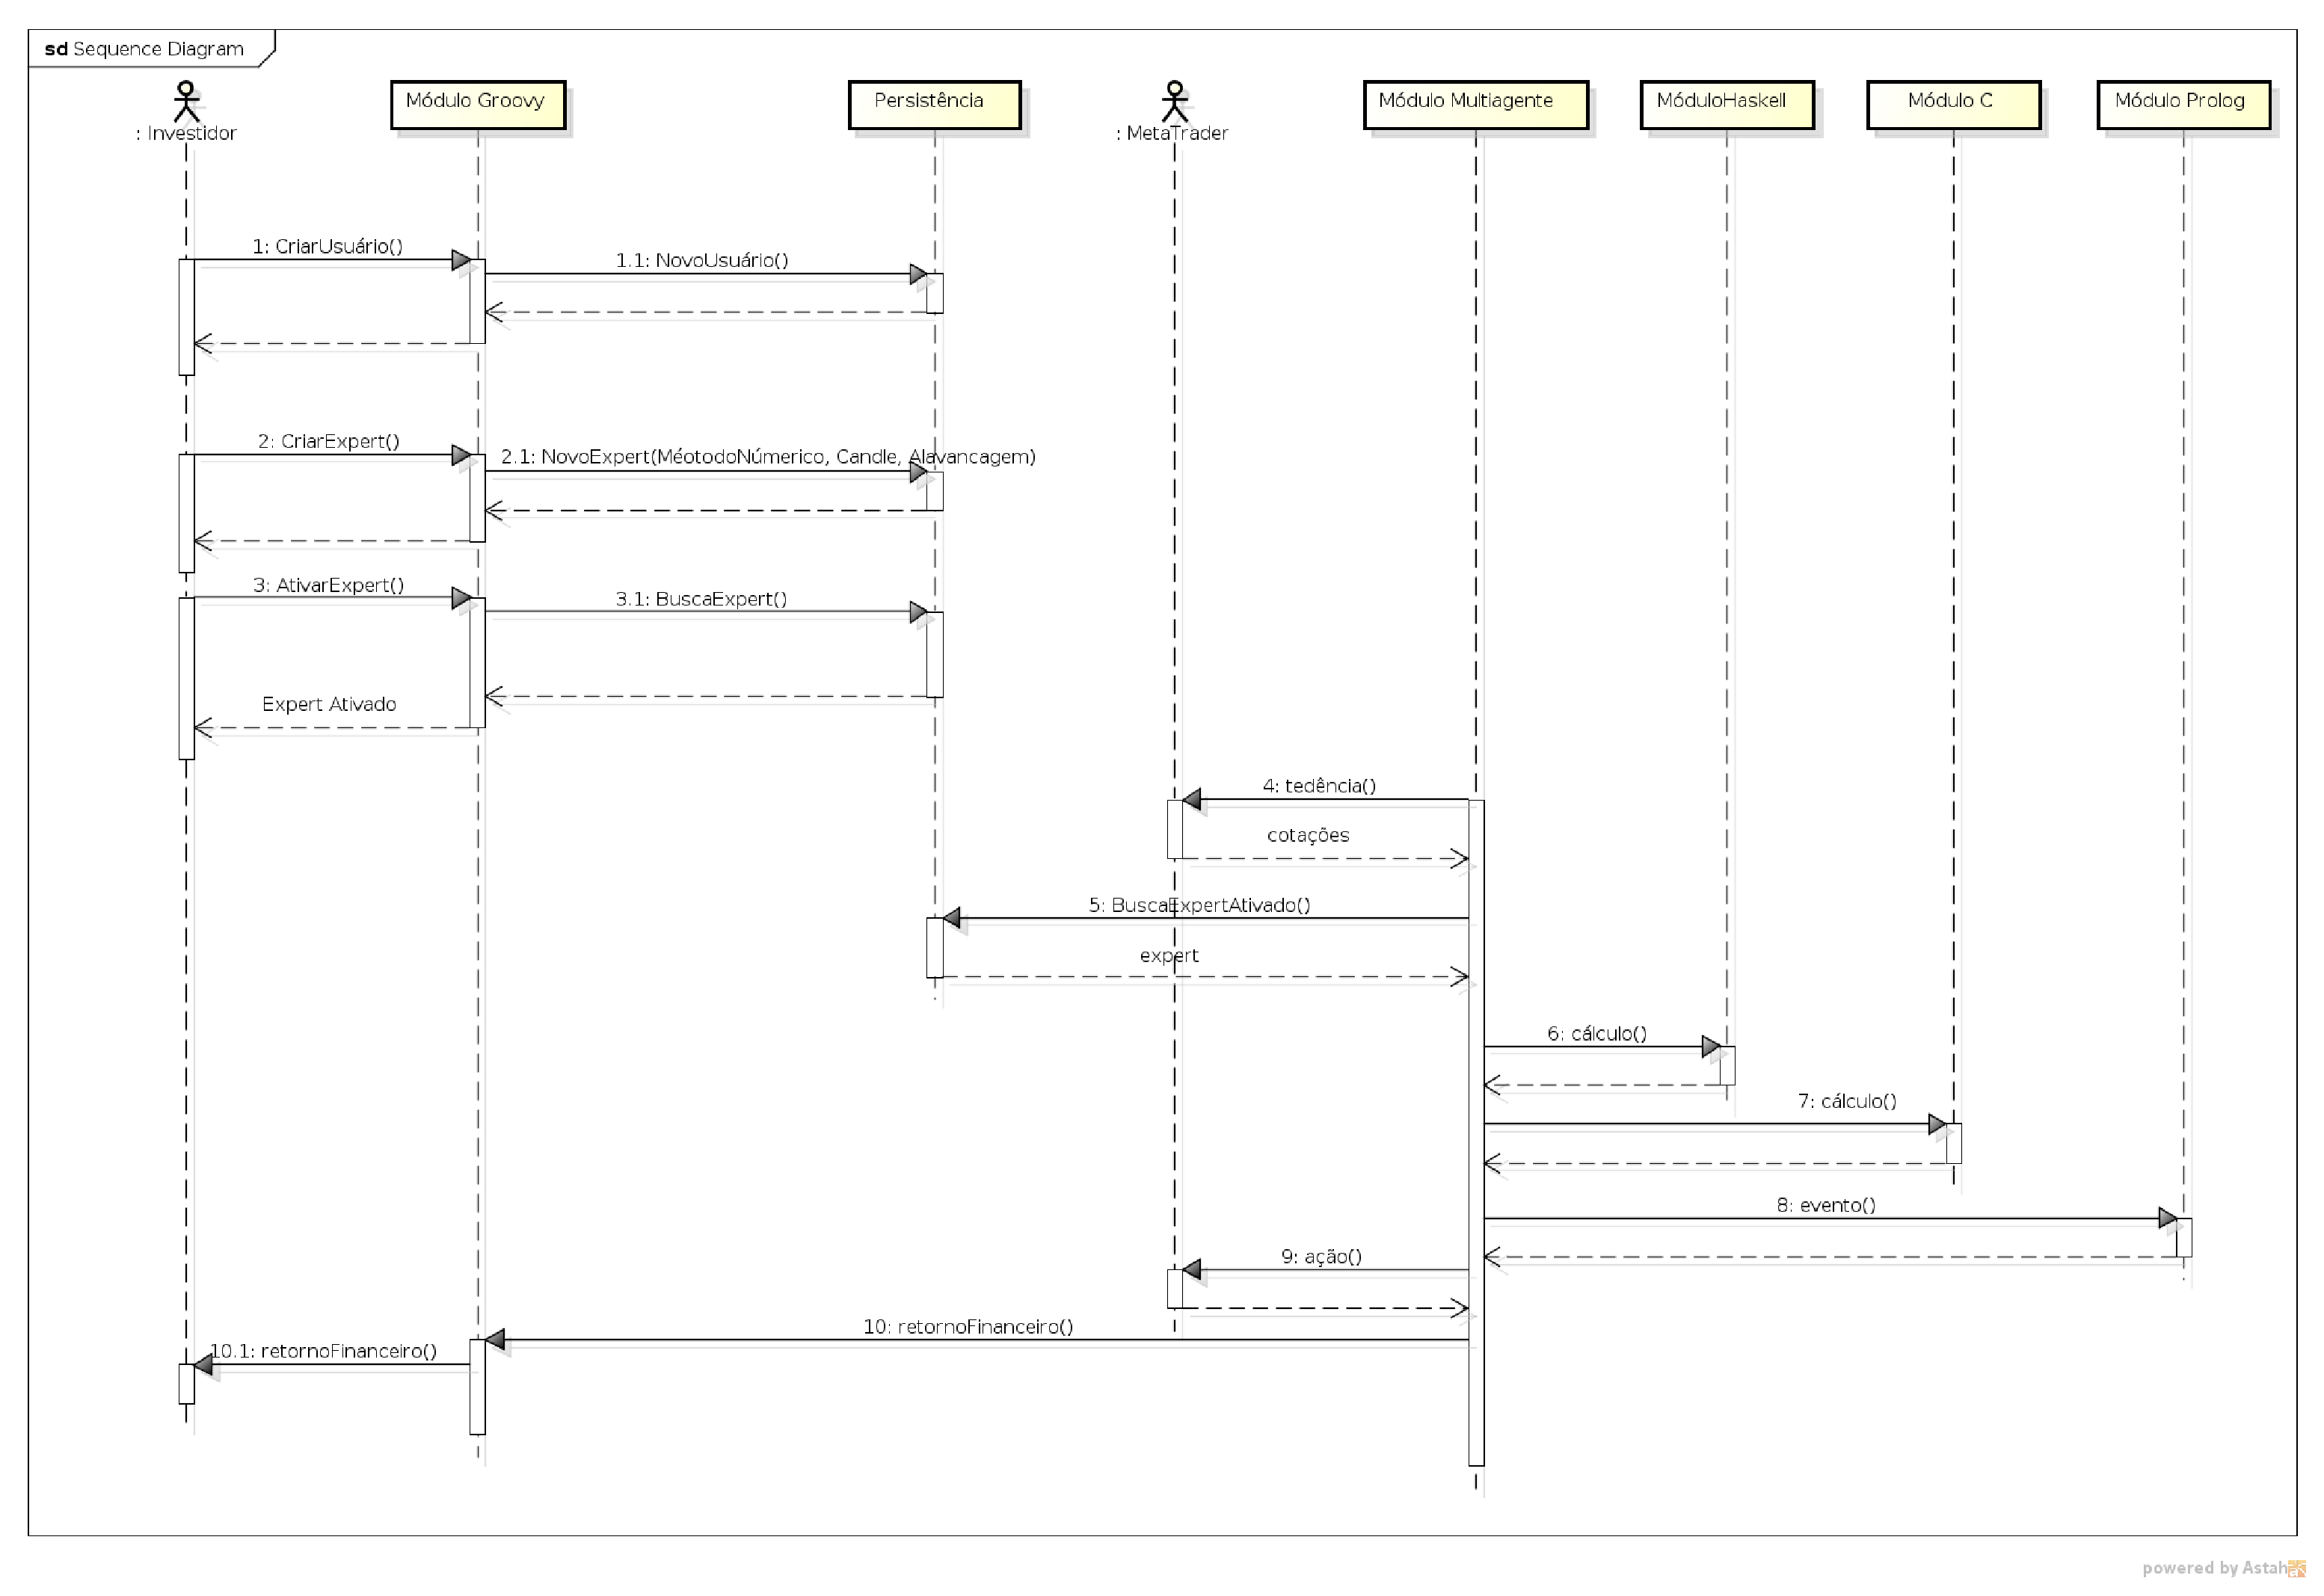
\includegraphics[width=0.9\textwidth]{figuras/sequencia}
\caption{Diagrama de Sequência InvestMVC} 
\label{sequencia}
\end{figure}

\section{Testes unitários e cobertura de código-fonte}
Esta seção evidencia o resultado dos testes unitários dos componentes Estruturado, Lógico, Funcional e Multiagente. Este resultado atende o objetivo específico 3 (apurar a cobertura de código por meio de ferramentas que implementam testes unitários) deste trabalho.
\subsection{Componente Funcional}

Foram realizados os testes unitários na linguagem haskell utilizando o \textit{framework} HUnit. O \textit{framework} não fornece a cobertura de código-fonte, mas é possível visualizar a quantidade de casos de teste, quantidade de testes realizados, quantidade de erros e quantidade de falhas. Os resultados dos testes unitários dos métodos de Correlação de Pearson, Fibonacci e Mínimos Quadrados podem ser visualizados na Figura \ref{testeCorrelacaoHaskell}, \ref{testeFibonacciHaskell} e \ref{TesteMinimosHaskell}.

\begin{figure}[H]
\centering
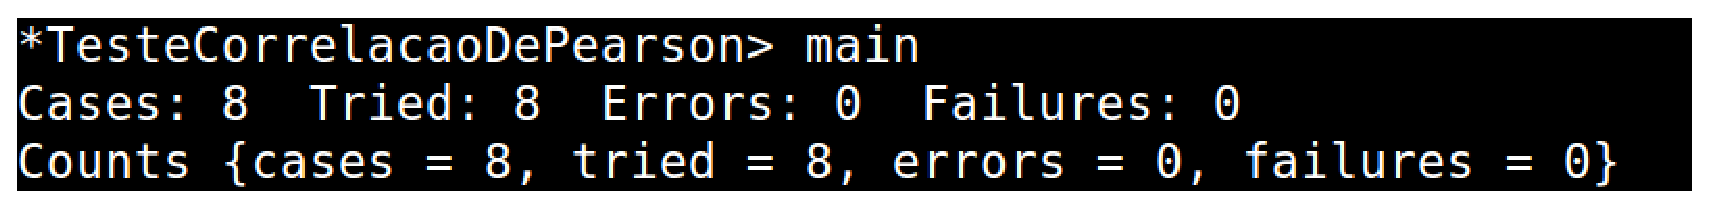
\includegraphics[width=0.9\textwidth]{figuras/testeCorrelacaoHaskell}
\caption{Resultado da Suíte de Teste do Método Correlação Linear}
\label{testeCorrelacaoHaskell}
\end{figure}

\begin{figure}[H]
\centering
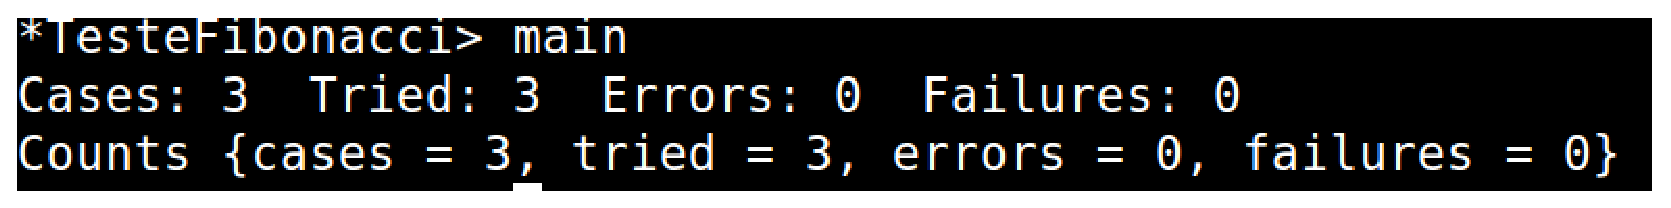
\includegraphics[width=0.9\textwidth]{figuras/testeFibonacciHaskell}
\caption{Resultado da Suíte de Teste do Método de Fibonacci}
\label{testeFibonacciHaskell}
\end{figure}

\begin{figure}[H]
\centering
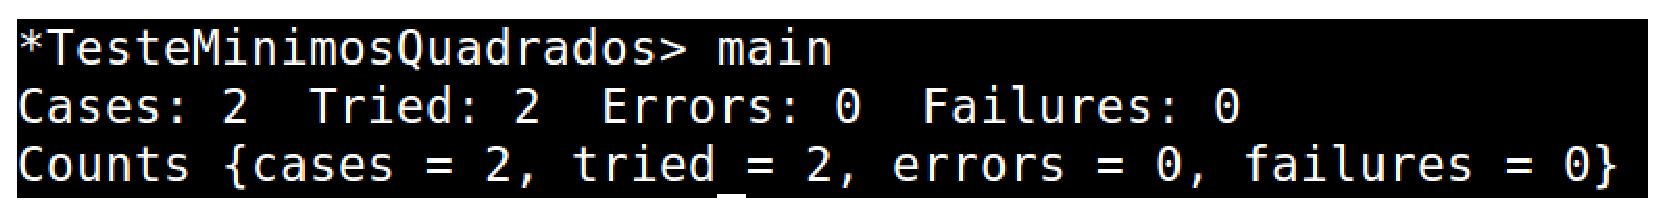
\includegraphics[width=0.9\textwidth]{figuras/TesteMinimosHaskell}
\caption{Resultado da Suíte de Teste do Método Mímimos Quadrados}
\label{TesteMinimosHaskell}
\end{figure}

Os códigos referentes aos testes unitários em linguagem Haskell, encontram-se no Apêndice \ref{ap:funcional}.

\subsection{Componente Estruturado}
Encontra-se no Apêndice \ref{ap:estruturado} , o código-fonte das Histórias de Usuário 13 (Método de Correlação Linear em linguagem C), 14 (Método de Fibonacci em linguagem C) e 15 (Método de Mínimos Quadrados em linguagem C). No mesmo apêndice, segue o teste
unitário de cada História de Usuário.

Na Figura \ref{testeC}, é possível ver o resultado da suite de teste do Componente Estruturado. A cobertura de código foi de 100\%.

\newpage
\begin{figure}[H]
\centering
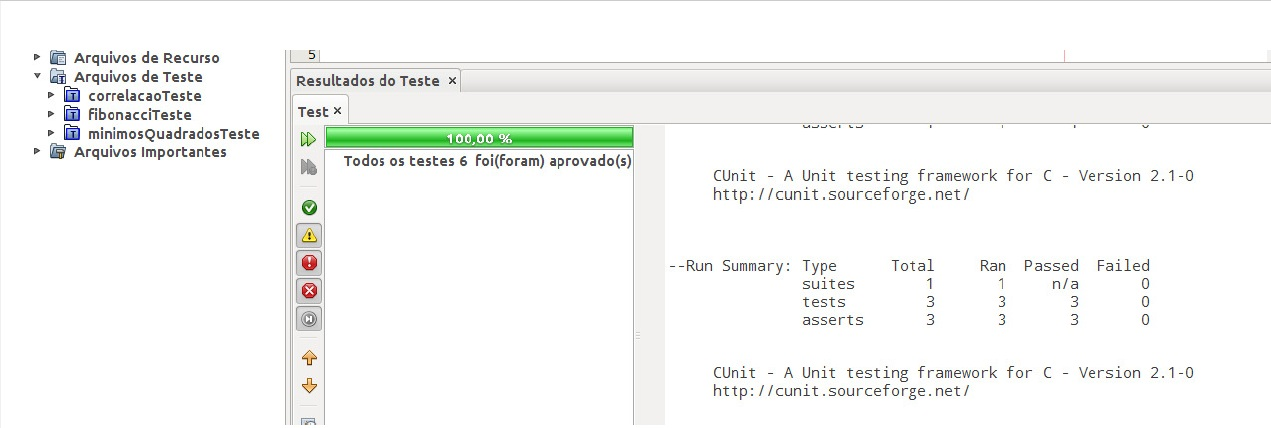
\includegraphics[width=0.9\textwidth]{figuras/testeC}
\caption{Cobertura de código-fonte Componente Estruturado}
\label{testeC}
\end{figure}

\subsection{Componente Lógico}
Foi utilizada a ferramenta Swi-prolog para realização dos testes unitários na linguagem Prolog. Não foi possível obter a cobertura de código-fonte da linguagem prolog utilizando a ferramenta Swi-prolog (os testes ficaram com cobertura fixa em 4.5). Entretanto, os testes foram realizados com sucesso, conforme pode ser visualizado nas Figuras \ref{prologTeste1} e \ref{prologTeste2}. 

\begin{figure}[H]
\centering
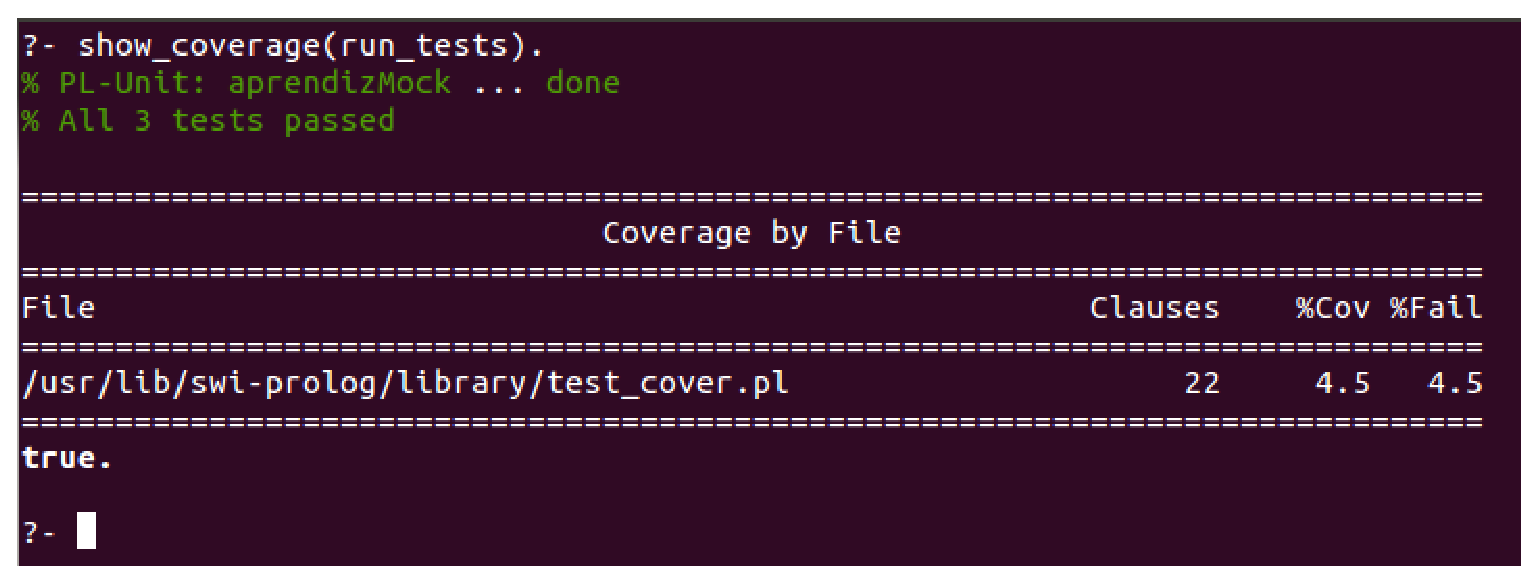
\includegraphics[width=0.9\textwidth]{figuras/prologTeste1}
\caption{Suíte de teste da base aprendiz.pl}
\label{prologTeste1}
\end{figure}

\begin{figure}[H]
\centering
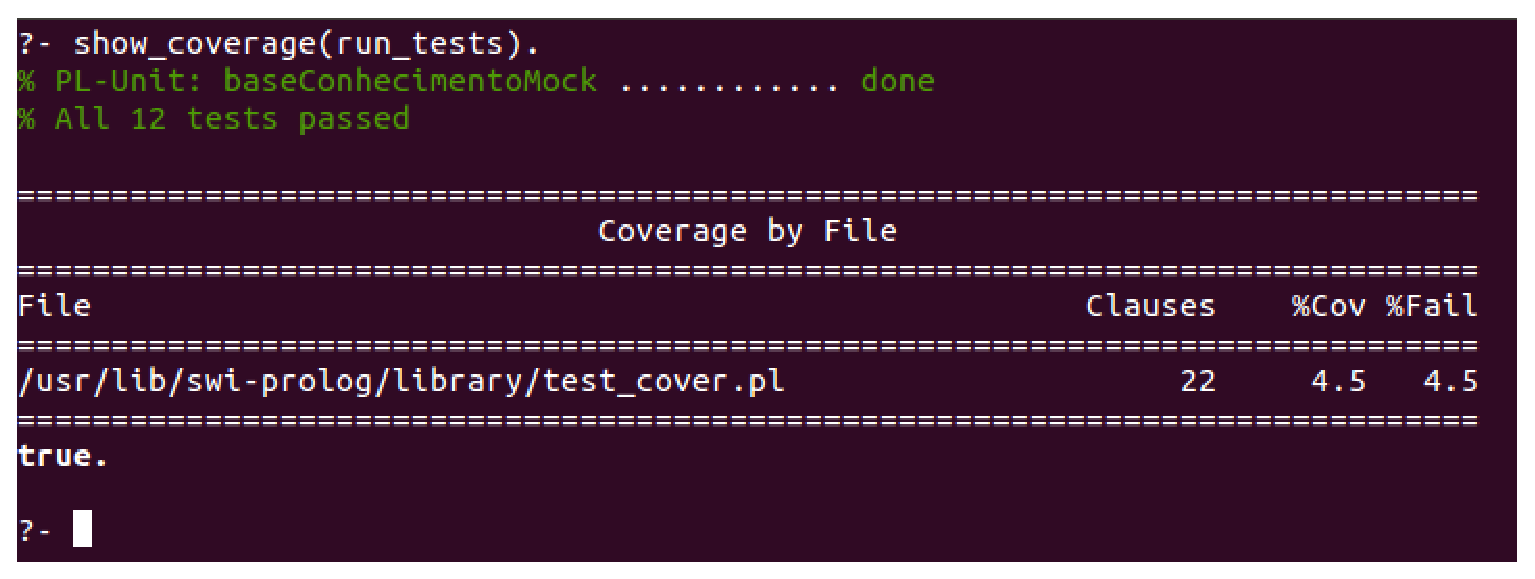
\includegraphics[width=0.9\textwidth]{figuras/prologTeste2}
\caption{Suíte de teste da base de conhecimento}
\label{prologTeste2}
\end{figure}

Os códigos referentes aos testes unitários em linguagem Prolog, bem como a implementação da base de conhecimento, encontram-se no Apêndice \ref{ap:logico}.

\subsection{Componente Multiagente}
Foram utilizados os frameworks Junit e Easy-mock para realização dos testes unitários na linguagem Java. Para obter a cobertura de código-fonte, foi utilizada a ferramenta Eclemma. Obteve-se uma cobertura de código-fonte de 84.8\% nos testes unitários, conforme pode ser visualizado na Figura \ref{eclemmaSMA}. 

\begin{figure}[H]
\centering
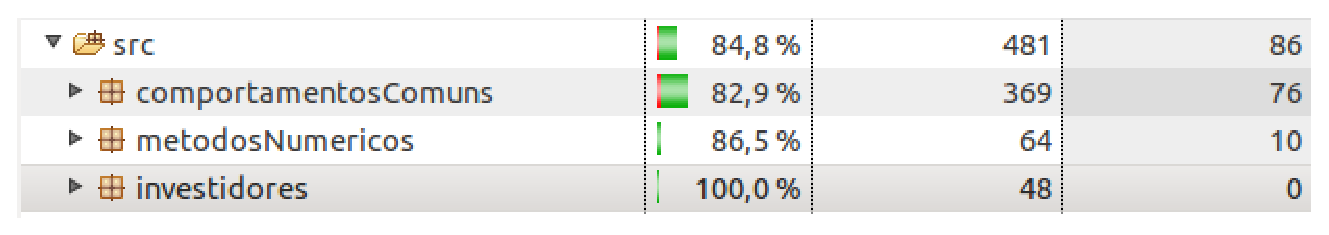
\includegraphics[width=0.9\textwidth]{figuras/eclemmaSMA}
\caption{Cobertura de Código dos pacotes do Componente Multiagentes}
\label{eclemmaSMA}
\end{figure}

O comportamento dos agentes são executados por meio dos métodos \textit{actions} e muitos  comportamentos precisavam de um tempo de até 6 segundos para serem executados. Devido a isso, os testes unitários quebraram, pois nenhum comportamento era executado a tempo. Para tentar solucionar esse problema, foram colocados \textit{delays} para que o tempo fosse ajustado, viabilizando a comunicação entre os agentes. A execução dos testes demorou mais de 18 (dezoito) segundos conforme pode ser visualizado no  canto superior esquerdo da Figura \ref{eclemmaTodasClasses}. Apesar de todos os testes passarem pelo Junit e o Easy-mock com os \textit{delays}, a ferramenta Eclemma não registrava a cobertura de código dos métodos \textit{actions}. Assim, esses métodos foram desconsiderados no percentual de cobertura de código-fonte.

\newpage
\begin{figure}[H]
\centering
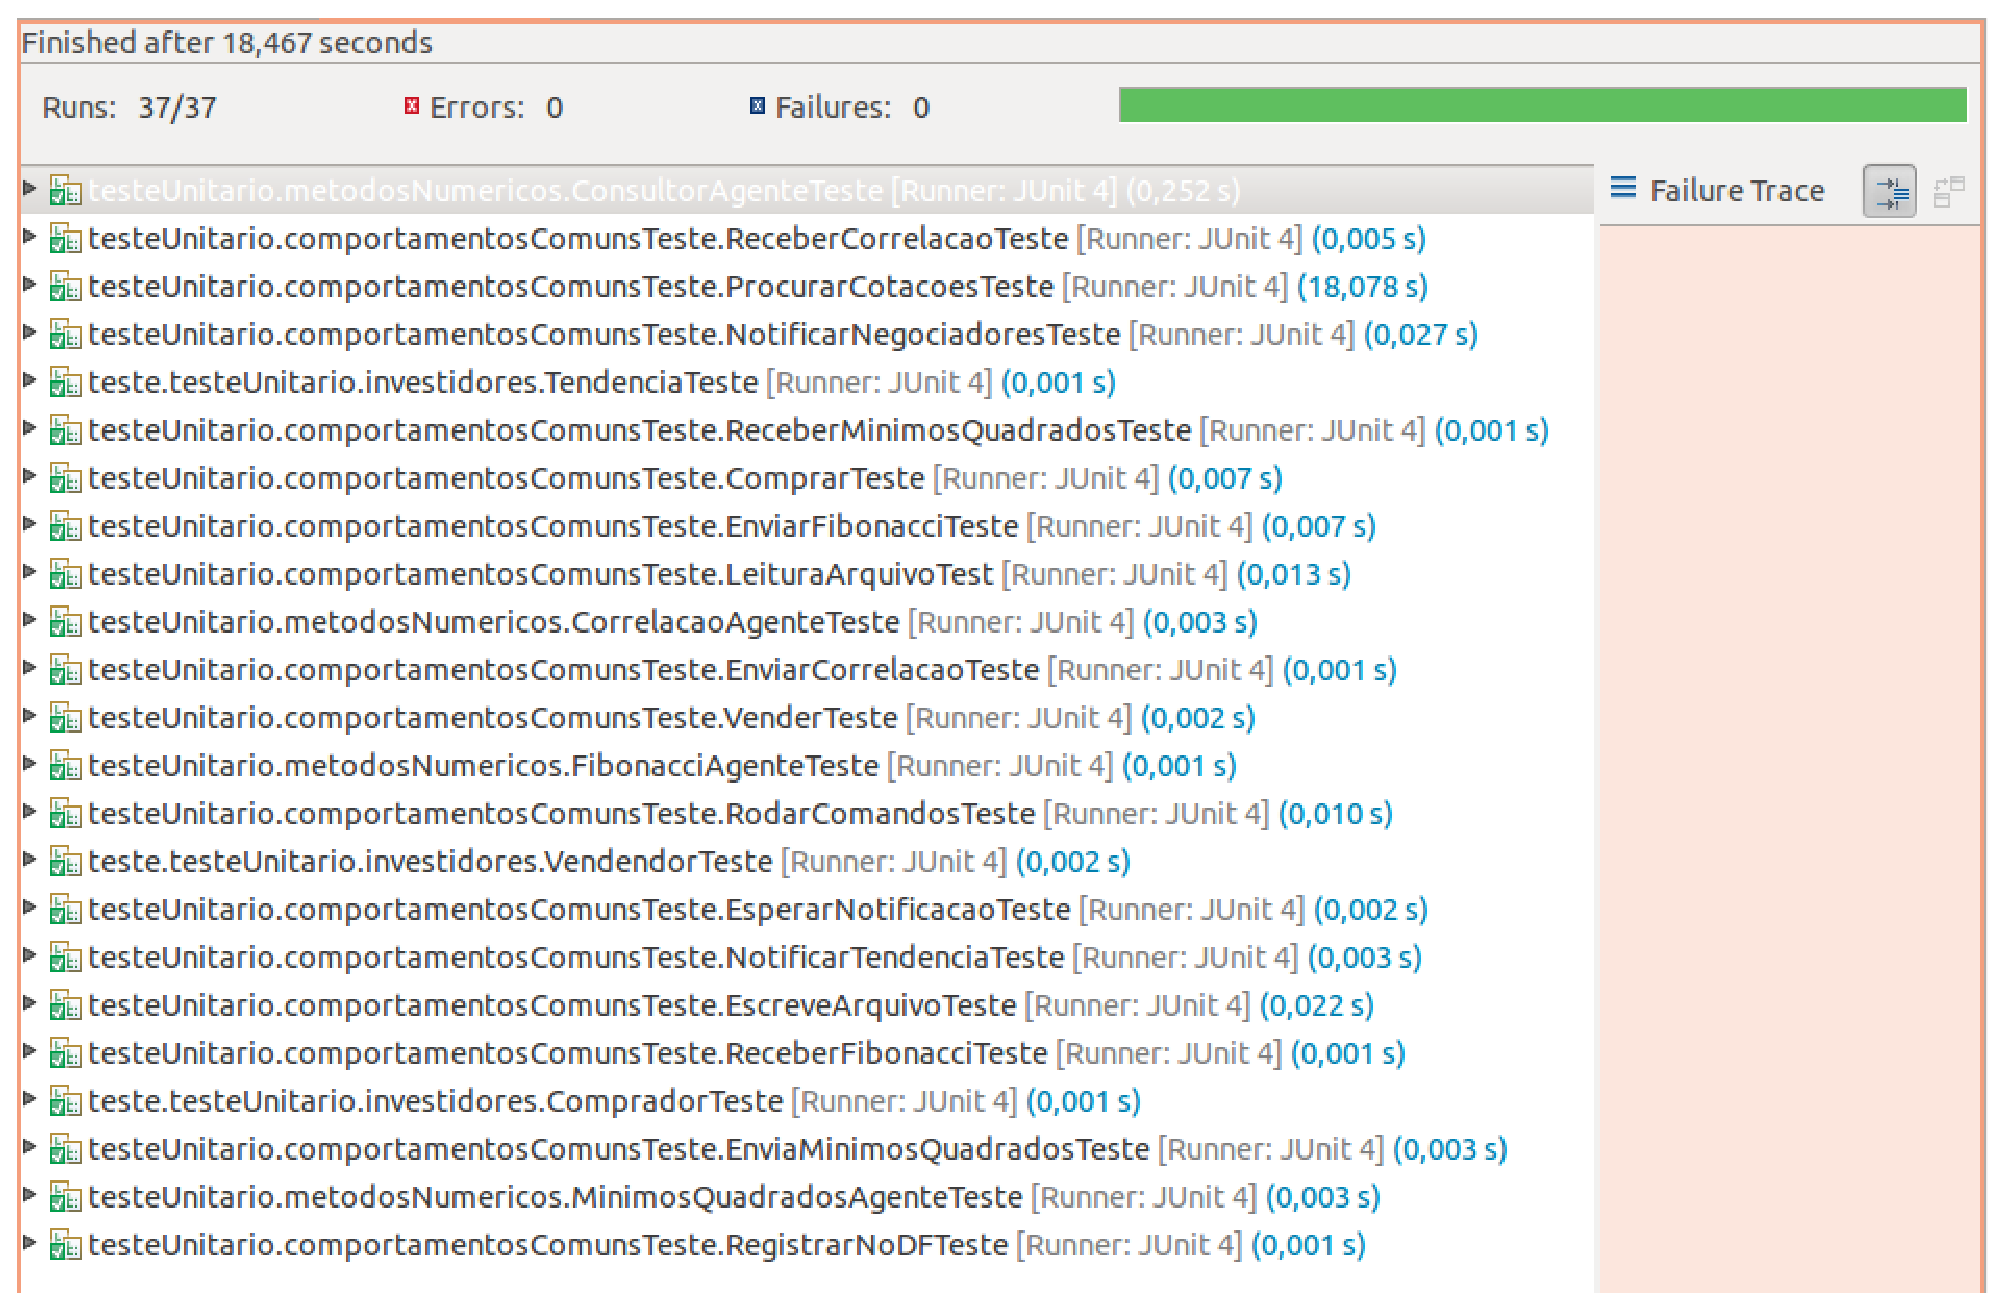
\includegraphics[width=0.9\textwidth]{figuras/eclemmaTodasClasses}
\caption{Suite de teste do Componente Multiagente}
\label{eclemmaTodasClasses}
\end{figure}

As classes de teste mais significativas encontram-se no Apêndice \ref{ap:sma}.

\section{Análise Estática de Código-fonte}
Esta seção apresenta o resultado da qualidade de código-fonte  do componente Multiagente, através da realização de análise estática e interpretação de métricas de qualidade de código-fonte. O resultado atende o objetivo específico 4 (realizar análise estática do código-fonte do componente Multiagente) deste trabalho. Não é objetivo deste trabalho evidenciar as relações entre as métricas como, por exemplo, a alta coesão tender a gerar um baixo acoplamento.

\subsection{Definição das Métricas de Qualidade de Código-fonte}
Para realizar a interpretação das métricas de qualidade de código-fonte, escolheu-se os valores de referência de acordo com a dissertação de \cite{filho}. Segundo ele, os valores foram obtidos baseando-se nos resultados da análise de um ou mais "projetos
modelo", analisados no Capítulo 4 da tese de \citeonline{meirelles2013}.

Segundo \citeonline{braga2012}, métricas estruturais de tamanho e profundidade são boas referências para saber se um código está com uma qualidade aceitável. Diante disso, foram escolhidas de forma empírica as métricas estruturais de coesão, acoplamento e complexidade ciclomática. As métricas de tamanho escolhidas foram número de parâmetros públicos e número de parâmetros por método. Por fim, escolheu-se a métrica de profundidade herança.

\subsection{Qualidade de código-fonte do software InvestMVC}
Foi realizada a análise estática de código-fonte no intuito de obter a qualidade de código-fonte do componente Multiagente. A Figura \ref{analiseinicial} revela o resultado da primeira análise estática. Percebe-se que a métrica número de parâmetros públicos (NPA) ficou com nível regular no pacote investidores. Com esse resultado, o código foi refatorado e o pacote investidores saiu do nível regular para o nível bom, conforme consta na Figura \ref{analisefinal}. Além disso, foi atribuida uma menor responsabilidade para o agente tendência no pacote comportamentosComuns e com isso, a complexidade ciclomática (ACCM) nesse pacote evoluiu de um nível bom para excelente. No Apêndice \ref{ap:analise}, é possível visualizar os resultados da análise estática de código-fonte de forma mais detalhada, pois os resultados de cada classe são evidenciados.

\begin{figure}[H]
\centering
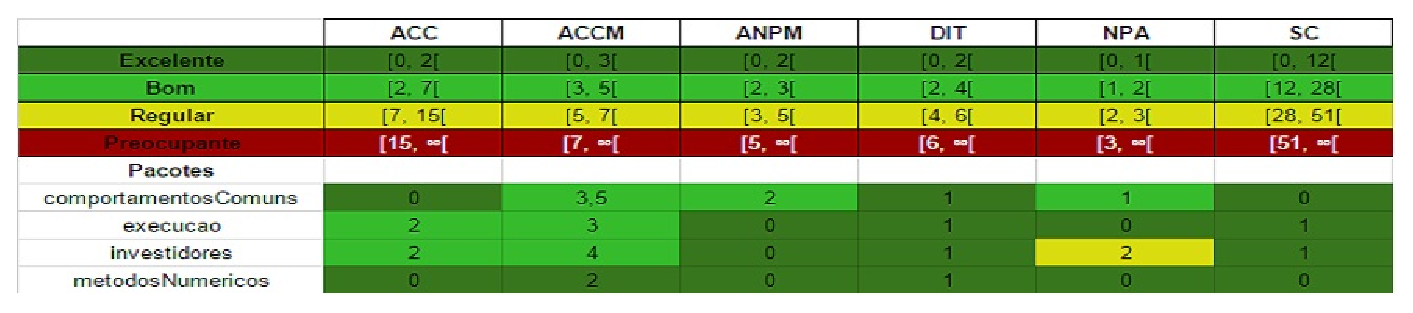
\includegraphics[width=0.9\textwidth]{figuras/analiseinicial}
\caption{Primeiro resultado da análise estática de código-fonte do componente Multiagente}
\label{analiseinicial}
\end{figure}

\begin{figure}[H]
\centering
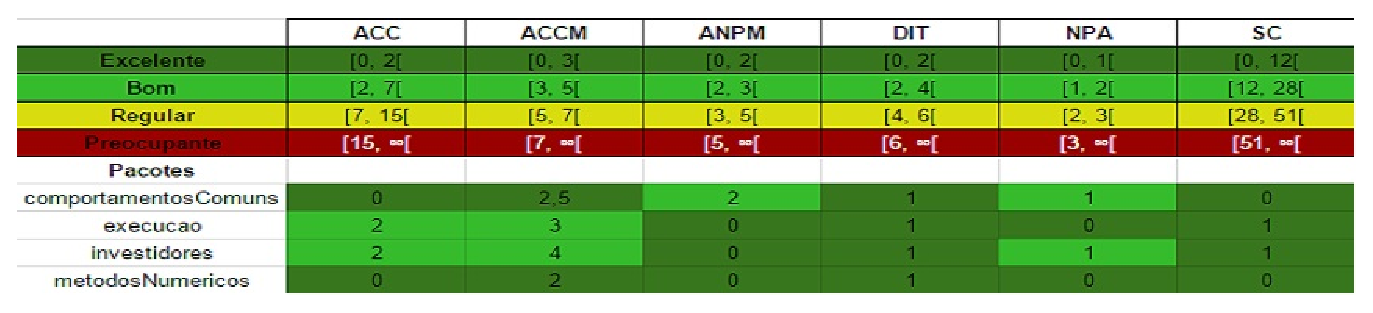
\includegraphics[width=0.9\textwidth]{figuras/analisefinal}
\caption{Segundo resultado da análise estática de código-fonte do componente Multiagente}
\label{analisefinal}
\end{figure}

\section{Comparação entre resultados monetários}
Esta seção evidencia o resultado dos rendimentos monetários do software InvestMVC e do \textit{expert} implementado em MQL. Os parâmetros (projeto, coleta dos dados, interpretação, validação) para comparar os valores monetários em dólares americanos dos produtos de software, foram definidos na metodologia. O período de coleta dos resultados monetários foi de 18 de Maio de 2015 à 12 de Junho de 2015 (20 dias de negociações, 24 horas por dia, sem contar sábados e domingos). O resultado atende o objetivo específico 5 (comparar resultados financeiros obtidos pelo software InvestMVC com os \textit{experts} tradicionais implementados em linguagem MQL) deste trabalho.

Utilizou-se o gráfico de linhas e de barras para evidenciar os resultados monetários, bem como o desvio padrão amostral e o método de Correlação Linear para evidenciar o resultados do tempo de entrada das operações. O relatório completo das negociações, encontra-se no Apêndice \ref{ap:historico}.


\subsection{Resultados monetários InvestMVC}
O software InvestMVC ficou rodando no Mercado de Moedas durante 20 dias de negociações e fez 19 operações. Dessas 19 operações, 8 (oito) operações tiveram lucro, o que evidencia um índice de acerto de 42.10\%. Apesar do índice de acerto ter sido inferior a 50\%, o software InvestMVC obteve um lucro de 120.58 USD (cento e vinte dólares e cinquenta e oito centavos de dólares). Sendo assim, obteve-se um lucro de 12,58\% durante as operações.

A Figura \ref{rendimentoInvestMVC}, evidencia o resultado do gráfico das operações em função do rendimento do software InvestMVC.

\begin{figure}[H]
\centering
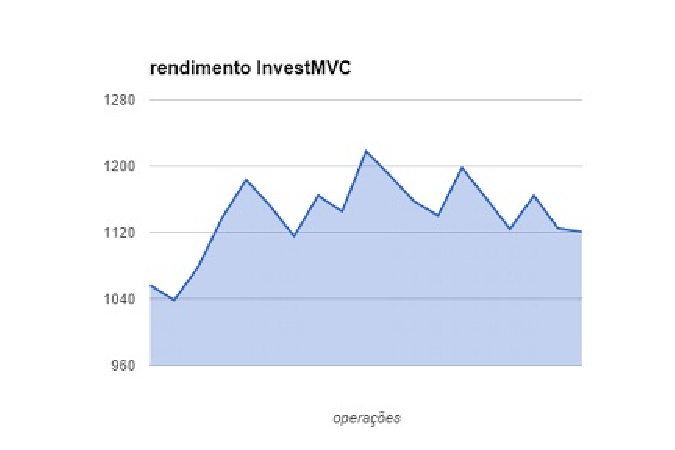
\includegraphics[width=0.9\textwidth]{figuras/rendimentoInvestMVC}
\caption{Gráfico de rendimento software InvestMVC}
\label{rendimentoInvestMVC}
\end{figure}

\subsection{Resultados monetários do \textit{expert} MQL}
Da mesma forma que o software InvestMVC, o \textit{expert} implementado em linguagem MQL também foi executado no Mercado de Moedas durante 20 dias e fez 19 operações. Dessas 19 operações, 8 (oito) negociações tiveram lucro, o que evidencia um índice de acerto de 42.10\%.

Foi obtido um lucro de 114.86 USD (cento e quatorze dólares e oitenta e seis centavos de dólares). Portanto, foi gerado um lucro de 11,48\% durante as operações. 

A Figura \ref{rendimentoInvestMQL}, evidencia o resultado do gráfico das operações em função do rendimento do \textit{expert} implementado em MQL.

\begin{figure}[H]
\centering
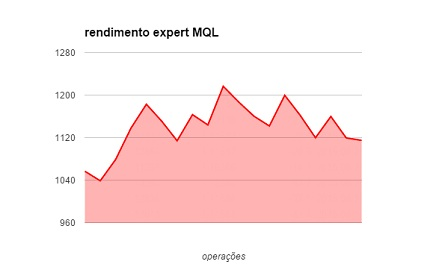
\includegraphics[width=0.9\textwidth]{figuras/rendimentoMQL}
\caption{Gráfico de rendimento do \textit{expert} implementado em MQL}
\label{rendimentoInvestMQL}
\end{figure}

\subsection{Resultados monetários obtidos em MQL \textit{versus} InvestMVC}
O tempo das operações (20 dias, 24 horas por dia), a quantidade de negociações (19) e índice de acerto nas operações (42.10\%) do \textit{expert} implementado em linguagem MQL foram iguais ao software InvestMVC.

O software InvestMVC obteve um lucro 5.72\% a mais que \textit{expert} implementado em MQL nos resultados monetários. 

A Figura \ref{rendimentoVersus} evidencia o gráfico de rendimento do \textit{expert} implementado em MQL (linha vermelha) e do software InvestMVC (linha azul). A linha vermelha e azul ficam juntas na maior parte do gráfico, o que evidencia que os resultados monetários foram semelhantes na maior parte do tempo.

\begin{figure}[H]
\centering
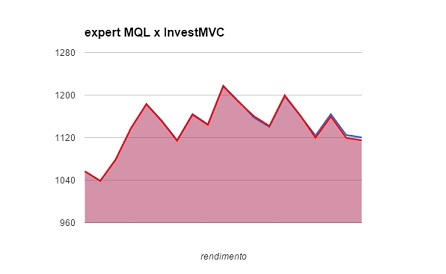
\includegraphics[width=0.9\textwidth]{figuras/rendimentoVersus}
\caption{Resultados monetários do \textit{expert} MQL e InvestMVC}
\label{rendimentoVersus}
\end{figure}

É possível que ambos produtos de software, obteveram lucros e perdas, mas o somatório dos lucros foi maior que o somatório das perdas.

A Figura \ref{graficoBarras} representa o gráfico da comparação dos resultados financeiros do \textit{expert} MQL e do software InvestMVC. As barras em vermelho e em azul representam, respectivamente, os rendimentos do \textit{expert} MQL e do software InvestMVC, no qual o eixo das abscissas representa as operações feitas pelos \textit{experts} implementados. Da mesma forma que no gráfico de linhas, é possível observar que os resultados monetários de ambos produtos de software ficaram bem próximos.


\begin{figure}[H]
\centering
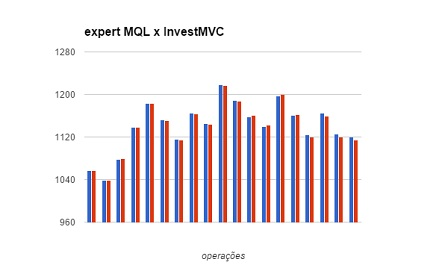
\includegraphics[width=0.7\textwidth]{figuras/graficoBarras}
\caption{Resultados monetários do \textit{expert} MQL e InvestMVC em gráfico de barras}
\label{graficoBarras}
\end{figure}

\subsection{Outros resultados associados ao rendimento monetário}

Verificou-se o horário exato em que foram feitas as operações do expert MQL e do software InvestMVC no Mercado de Moedas. A Tabela \ref{horarios}, evidencia os horários de entrada das operações, ou seja, o horário exato em que foi emitida uma ordem de compra ou venda.

\begin{center}
\begin{longtable}{| p{8cm} | p{8cm} |}
\caption{Horário de entrada no Mercado de Moedas \textit{expert} MQL e software InvestMVC} \\
\hline
\textbf{Horário operação \textit{expert} MQL} & \textbf{Horário Operação software InvestMVC} \\ \hline
\endfirsthead
\multicolumn{2}{c}%
{\tablename\ \thetable\ -- \textit{Continuação da página anterior}} \\
\hline
\textbf{Horário operação \textit{expert} MQL} & \textbf{Horário Operação software InvestMVC} \\ \hline
\endhead
\hline \multicolumn{2}{c}{\textit{Continuação na próxima página}} \\
\endfoot
\hline
\endlastfoot
	
2015.05.18 18:01:02 & 2015.05.18 18:01:17\\ \hline
2015.05.19 06:06:08 & 2015.05.19 06:06:34\\ \hline
2015.05.19 09:50:07 & 2015.05.19 09:50:01\\ \hline
2015.05.19 16:33:47 & 2015.05.19 16:33:56\\ \hline
2015.06.01 05:29:26 & 2015.06.01 05:29:34\\ \hline
2015.06.01 12:41:19 & 2015.06.01 12:41:22\\ \hline
2015.06.01 20:58:47 & 2015.06.01 20:58:55\\ \hline
2015.06.03 10:53:32 & 2015.06.03 10:53:35\\ \hline
2015.06.04 10:39:09 & 2015.06.04 10:39:31\\ \hline
2015.06.04 17:00:17 & 2015.06.04 17:00:33\\ \hline
2015.06.05 02:41:23 & 2015.06.05 02:41:21\\ \hline
2015.06.05 15:29:45 & 2015.06.05 15:29:56\\ \hline
2015.06.08 01:30:42 & 2015.06.08 01:30:43\\ \hline
2015.06.09 10:53:21 & 2015.06.09 10:53:22\\ \hline
2015.06.09 16:19:47 & 2015.06.09 16:19:43\\ \hline
2015.06.11 15:32:39 & 2015.06.11 15:32:44\\ \hline
2015.06.12 07:50:36 & 2015.06.12 07:50:46\\ \hline
2015.06.12 13:03:29 & 2015.06.12 13:03:43\\ \hline
2015.06.12 23:24:18 & 2015.06.12 23:24:22
\label{horarios}
\end{longtable}
\end{center}

Foi calculado o desvio padrão amostral dos tempos de entrada do \textit{expert} MQL e do software InvestMVC e obteve-se um desvio de 4.23 segundos. Também foi calculado o coeficiente  de Correlação Linear dos tempos de entrada e obteve-se um coeficiente de 0.83.

O desvio de 4.23 segundos é considerado relativamente alto, visto que em tese ambos produtos de software deveriam entrar em pontos semelhantes e, portanto, também em tempos de entrada semelhantes. Segundo \citeonline{lopes2005}[pág.~134], o resultado de uma Correlação Linear é considerada como forte se for acima de 0.85. Portanto, o resultado da Correlação Linear é significativo, mas não é considerado como forte. 
